\documentclass[a4wide,11pt]{report}
\usepackage[dvips]{graphicx}
\usepackage{url}
\usepackage{epstopdf}
\usepackage{float}
\usepackage{csvsimple}
\usepackage{hyperref}
\usepackage{longtable}
\usepackage{fancyhdr}
\pagestyle{fancy}
\usepackage{graphicx}

\begin{document}

\title{OpenStack Community Activity Report\\
      October-December, 2014 \\
      Report sponsored by the OpenStack Foundation\\
      %~~\\~~\\  \includegraphics[scale=.35]{openstack.eps}       \\
        ~~\\~~\\  
\includegraphics[scale=.35]{logo.eps}       \\}




\maketitle


\newpage
~~\\~\\~\\~\\
\begin{tabular}{p{5cm}p{10cm}}
AUTHOR & Daniel Izquierdo Cort\'azar \\
       & Chief Data Officer  \\
       & dizquierdo@bitergia.com \\
       &  \\
AUTHOR  & Stefano Maffulli \\
        & OpenStack Community Manager \\
        & stefano@openstack.org \\
\end{tabular}

~~\\~~\\

We would like to thank the effort of the following people their effort to provide feedback and validation process. 

~~\\
~~\\

\begin{tabular}{p{5cm}p{10cm}}

\end{tabular}

~~\\
~~\\

Finally, this report would not exist without the effort of the people involved in the development of the \href{https://activity.openstack.org/dash}{OpenStack Activity Board}, \href{http://metricsgrimoire.github.io}{Grimoire toolset} and the feedback of the people in the development mailing list of the OpenStack Foundation.

~~\\
~~\\
~~\\
~~\\
~~\\
~~\\

%\begin{flushright}
%Text is available under the CC BY 3.0 License\\
%License available at \url{http://creativecommons.org/licenses/by/3.0/}
%\end{flushright}


%\rhead{Bitergia Report}
%\rhead{\includegraphics[scale=.15]{openstack.eps}
\includegraphics[scale=.15]{logo.eps}}
\rhead{
\includegraphics[scale=.15]{logo.eps}}
%\rhead{
\includegraphics[scale=.15]{logo.eps}}




\newpage

\begin{center}
\textbf{Executive Summary}
\end{center}



\setcounter{tocdepth}{4}
\setcounter{secnumdepth}{4}
\tableofcontents


\chapter{Overview of the Project}

\section{General Activity}



A more detailed information about the community activity ...


\begin{table}[H]
    \centering
    \begin{tabular}{c|c|c|}%
    \bfseries Data source & \bfseries Activity 365 days & \bfseries Change (wrt to prev. 365 days) % specify table head
    \csvreader[head to column names]{data/data_source_evolution.csv}{}% use head of csv as column names
    {\\\datasource & \netvalues ~ \metricsnames & \relativevalues\% }
    \end{tabular}
    \caption{Activity during the last 365 days and its evolution}
\end{table}



Focusing on the development activity, 


\begin{table}[H]
    \centering
    \begin{tabular}{c|r|}%
    \bfseries Integrated Project & \bfseries Commits % specify table head
    \csvreader[head to column names]{data/integrated_projects_commits.csv}{}% use head of csv as column names
    {\\\projects & \commits }
    \end{tabular}
    \caption{Last quarter integrated projects number of commits}
\end{table}


\section{Development and Conversations}

Regarding to the community, developers are divided into three main sets, core, regular and occasional\footnote{Contributing developers are characterized as core, regular and occasional depending on their activity in the git repositories. The classification is built by sorting contributors by their total number of commits; we sum the total commits per each individual contributors: the individuals whose commits sum up to 80\% of the total number of commits in the quarter are the core contributors in that quarter. The regular contributors are those whose commits sum up to 95\% of the total. The others are the occasional contributors.}. 


\begin{figure}[H]
    \centering
    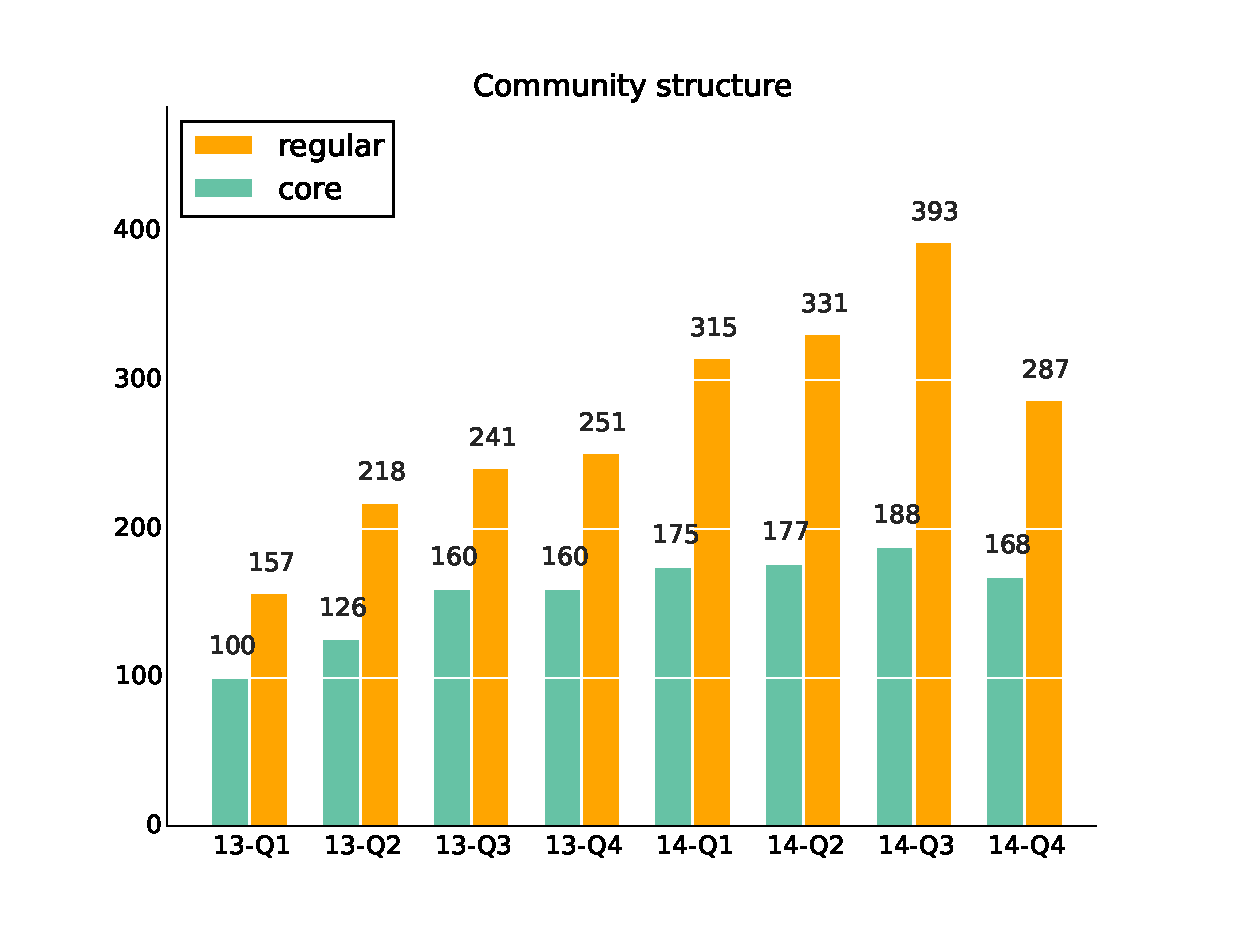
\includegraphics[scale=.35]{figs/onion.eps}
    \caption{Evolution of the last 8 quarters of the core, regular and occasional developers (Git activity)}
\end{figure}

\begin{table}[H]
    \centering
    \begin{tabular}{l|r|r|r|}%
    \bfseries Period & \bfseries Core & \bfseries Regular & \bfseries Occasional% specify table head
    \csvreader[head to column names]{data/onion_model.csv}{}% use head of csv as column names
    {\\\labels & \core & \regular & \occasional}
    \end{tabular}
    \caption{Characterization of developers by their total contribution to the OpenStack projects}
\end{table}


The mean number of developers per month 

\begin{figure}[H]
    \centering
    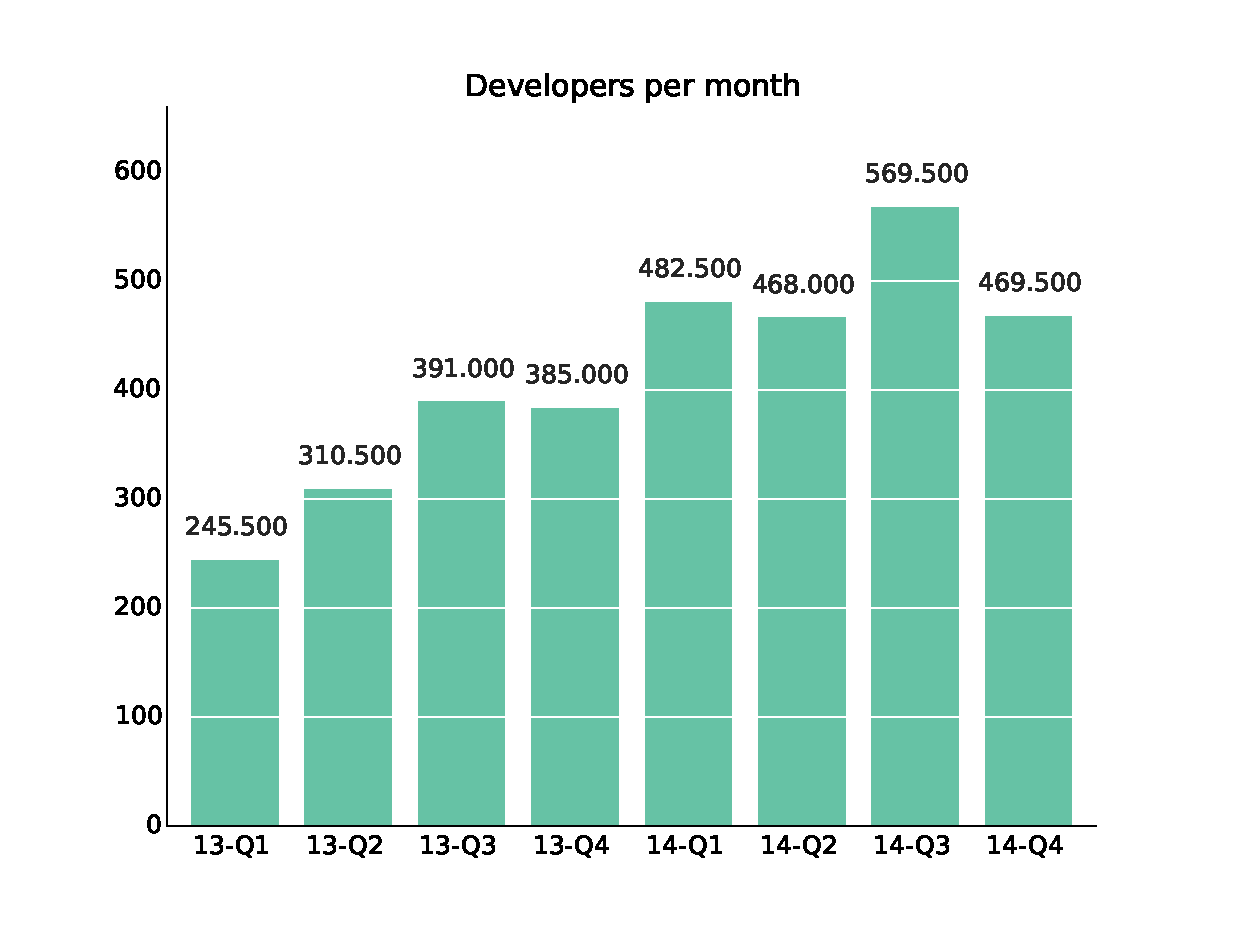
\includegraphics[scale=.35]{figs/authors_month.eps}
\caption{Number of developers per month in mean for each quarter}
\end{figure}


\section{Efficiency}



%Difference between integrated and non-integrated projects in terms of efficiency closing issues, and time to review, mean and median.

%Areas of knowledge per company in the integrated projects.

%Newer projects tend to be faster closing issues, or at least, they are improving their times to review and attend tickets. 

Two metrics have been identified to measure efficiency: the review efficiency index (REI) and the Time to Merge. REI is measured as the number of closed (merged or abandoned) changesets out of the submitted changesets in a given period. Time to Merge is measured as the time since a review is submitted until this is closed. Typical BMI values in the OpenStack Integrated projects rounds a 0.75, what indicates that for 100 opened changesets in a period, the community closes 75. Besides, the median Time to Merge is of 7.82, having an increase from the previous period.

%Explain what 'time to review' means

\begin{table}[H]
    \centering
    \begin{tabular}{c|c|c|c|}%
    \bfseries Integrated project & \bfseries REI & \bfseries TTM & \bfseries BMI % specify table head
    \csvreader[head to column names]{data/integrated_projects_efficiency.csv}{}% use head of csv as column names
    {\\\projects & \bmi  & \timereview & \bmiits ~ days}
    \end{tabular}
    \caption{Closed changesets out of opened changesets and median Time to Merge in Gerrit}
\end{table}


%And a detailed view of the evolution of the BMI during the last four quarters.

%\begin{figure}[H]
%\centering
%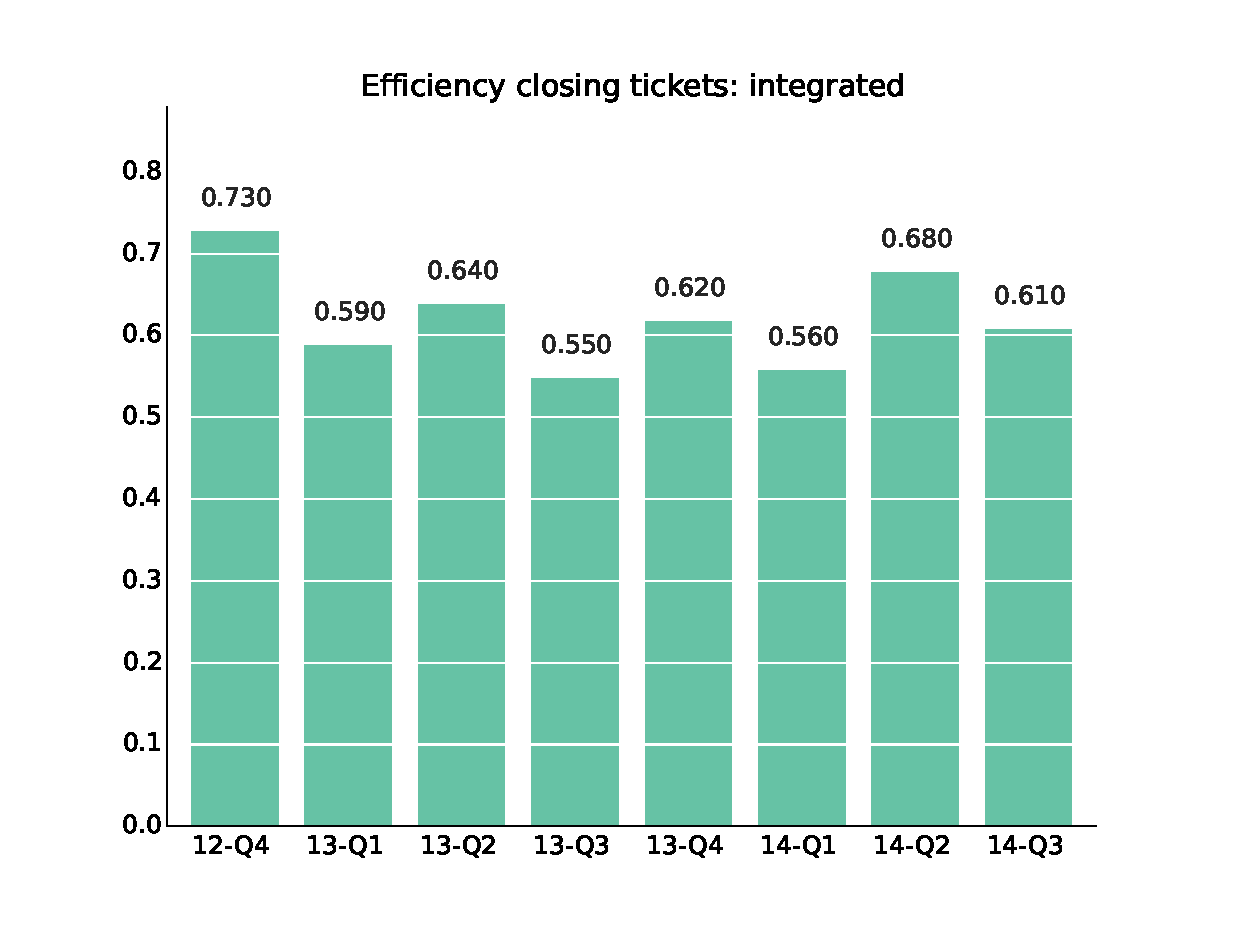
\includegraphics[scale=.35]{figs/bmiintegrated.eps}
%\caption{Backlog Management Index evolution for the Integrated projects}
%\end{figure}


%However, these numbers show that there is a gap of pending tickets opened that can be visualized at\footnote{dashboard url}. 

%Best project closing issues (with the best efficiency)
%Best project with the time to review
%Company leading most of the projects
%Projects with the highest number of developers

%Comparison of the activity of qaforums and mailing lists (qaforums is increasing, while mailing lists keep stable).

%Top threads (crowdest and with the highest number of issues)
%Top tags (topics) mentioned in the qaforums stuff
%Top visited questions and top commented questions from qaforums.


\chapter{Per Project break down}

This chapter aims at providing a detailed report on the activity of the OpenStack Foundation projects.
This is mainly focused on the activity per project as defined, stressing the point on the 'integrated' projects.

Each of the projects is divided into three sections and provides information from the last eight quarters.: 
\begin{itemize}
\item activity: centered in the following metrics: commits from git activity, submitted, merge and abandoned reviews from the review system and
opened and closed tickets from the issue tracking system. 
\item community: active core reviewers in gerrit, active authors in Git and top ten developers and top ten organizations contributing to the development in the last quarter.
of each project.
\item process: efficiency closing changesets, Time to Merge (mean and median), number of patchests (iterations) per changeset and study on the time waiting for a reviewer or submitter action in the patchset review process.
\end{itemize}


\newpage
\section{Overall OpenStack Programs}
\textbf{Activity}: Commits in Git, submitted, merged and abandoned reviews in Gerrit and opened and closed issues in Launchpad.


\begin{tabular}{p{7cm} p{5cm}}
    \vspace{0pt} 
    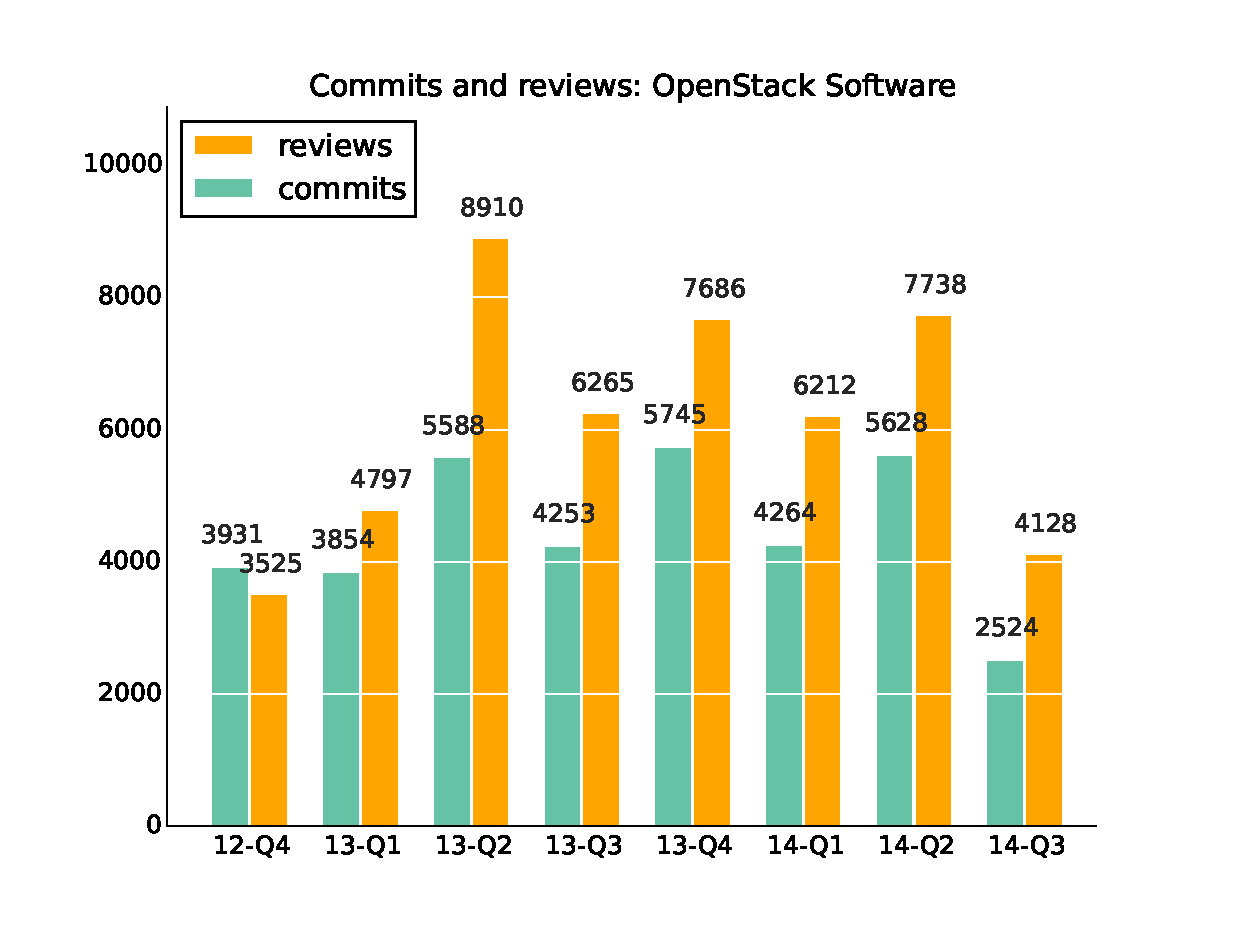
\includegraphics[scale=.35]{figs/commitsOpenStackSoftware.eps}
    & 
    \vspace{0pt}
    \begin{tabular}{l|r|r|}%
    \bfseries Period & \bfseries Commits & \bfseries Reviews% specify table head
    \csvreader[head to column names]{data/commitsOpenStackSoftware.csv}{}% use head of csv as column names
    {\\\labels & \commits & \submitted}
    \end{tabular}
\end{tabular}


\begin{tabular}{p{7cm} p{5cm}}
    \vspace{0pt} 
    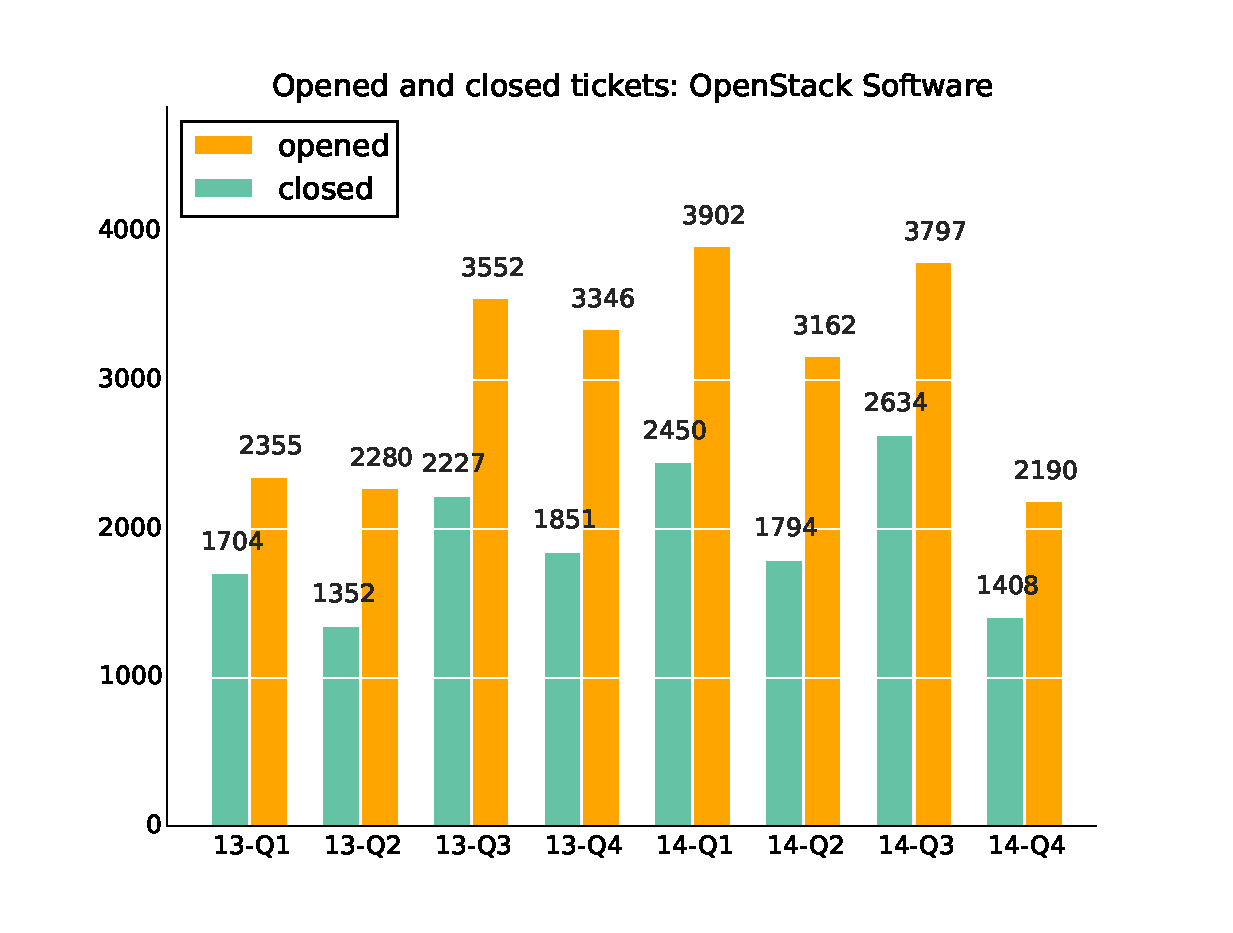
\includegraphics[scale=.35]{figs/closedOpenStackSoftware.eps}
    & 
    \vspace{0pt}
    \begin{tabular}{l|r|r|}%
    \bfseries Period & \bfseries Closed & \bfseries Opened% specify table head
    \csvreader[head to column names]{data/closedOpenStackSoftware.csv}{}% use head of csv as column names
    {\\\labels & \closed & \opened}
    \end{tabular}
\end{tabular}

\begin{tabular}{p{7cm} p{5cm}}
    \vspace{0pt} 
    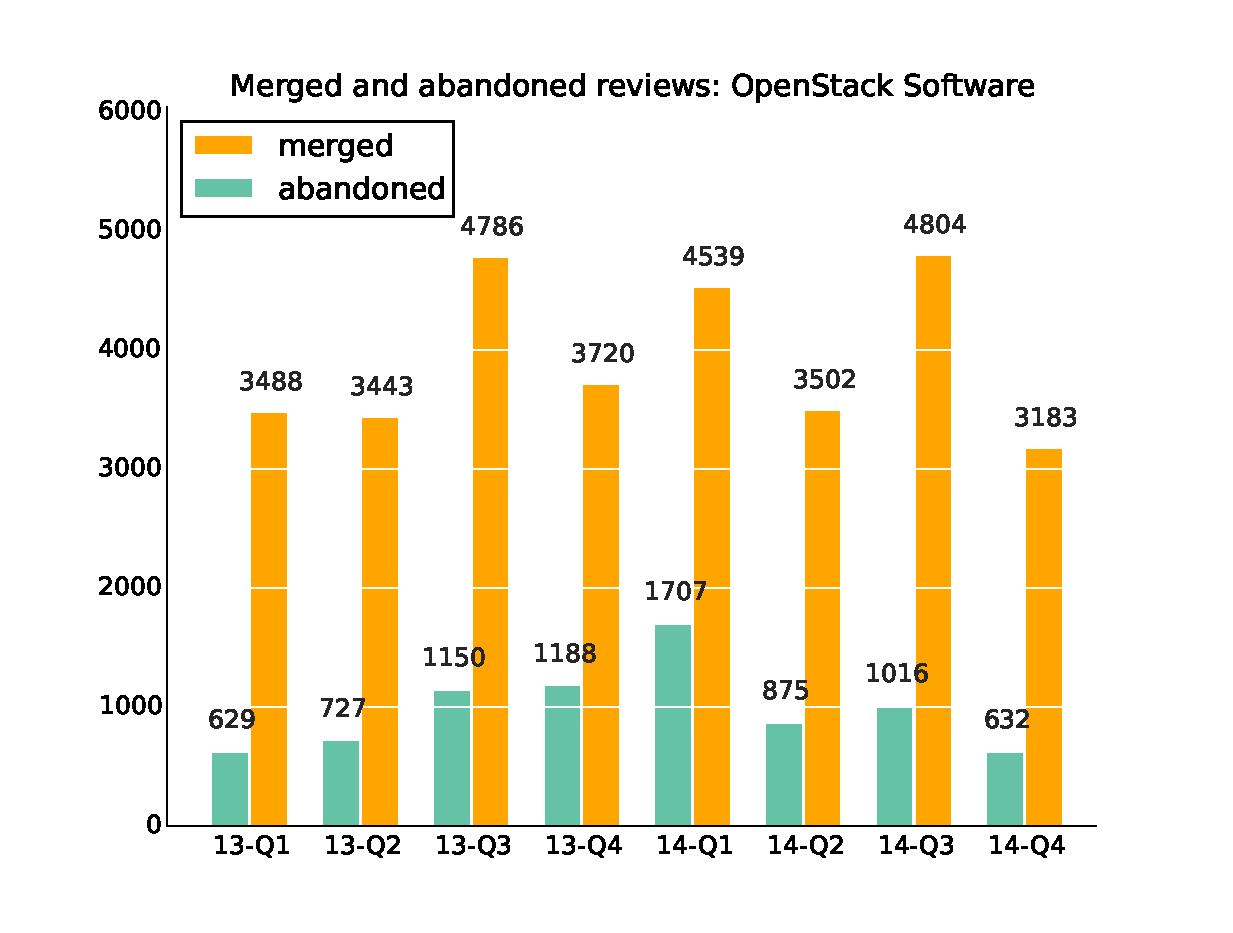
\includegraphics[scale=.35]{figs/submitted_reviewsOpenStackSoftware.eps}
    & 
    \vspace{0pt}
    \begin{tabular}{l|r|r|}%
    \bfseries Period & \bfseries Merged & \bfseries Abandoned % specify table head
    \csvreader[head to column names]{data/submitted_reviewsOpenStackSoftware.csv}{}% use head of csv as column names
    {\\\labels & \merged & \abandoned}
    \end{tabular}
\end{tabular}

\section{Community}
Active core reviewers in Gerrit, active authors in Git, top authors and organizations in the last quarter


\begin{tabular}{p{7cm} p{5cm}}
    \vspace{0pt} 
    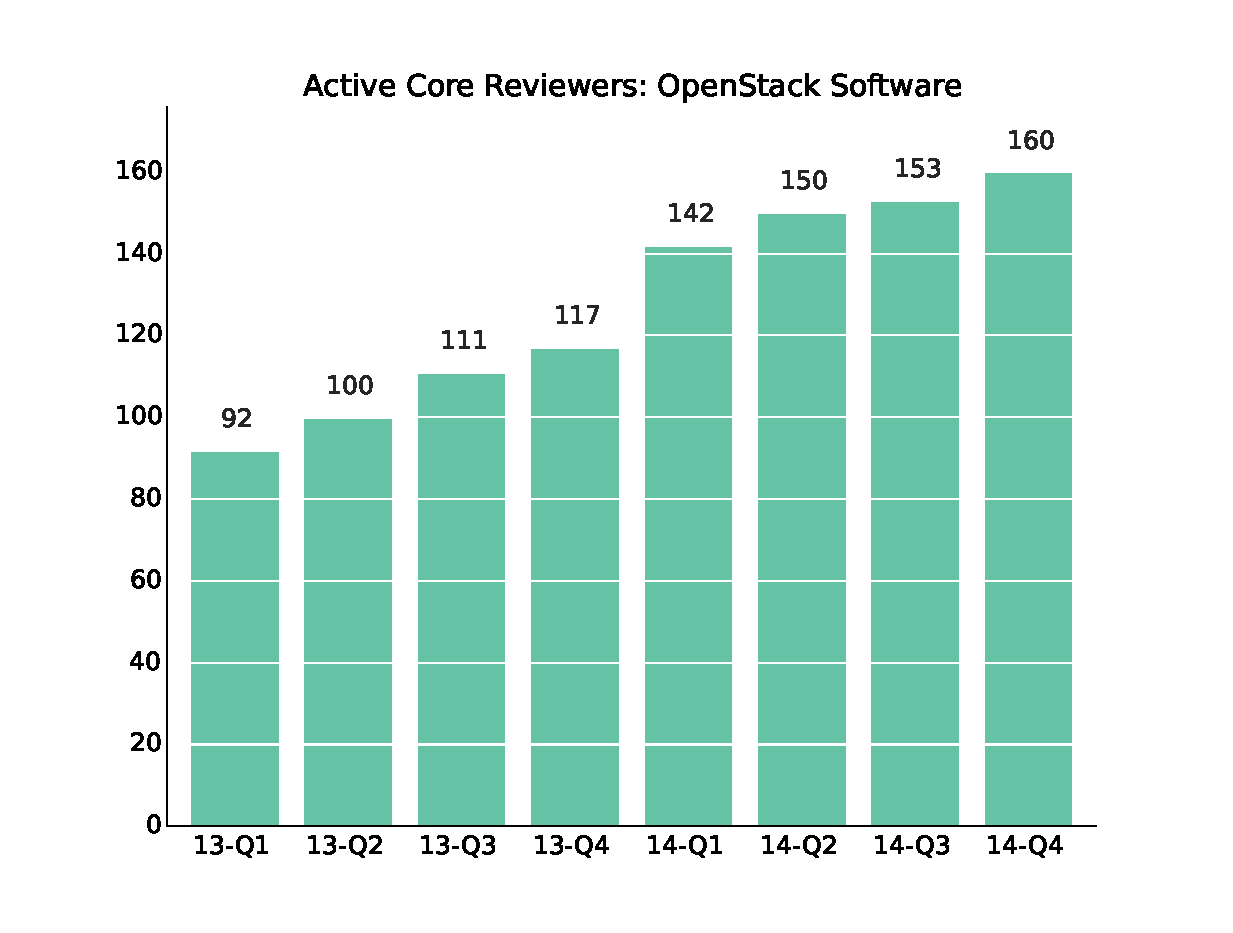
\includegraphics[scale=.35]{figs/active_core_scrOpenStackSoftware.eps}
    & 
    \vspace{0pt}
    \begin{tabular}{l|l}%
    \bfseries Period & \bfseries Active Core % specify table head
    \csvreader[head to column names]{data/active_core_scrOpenStackSoftware.csv}{}% use head of csv as column names
    {\\\labels & \activecorereviewers}
    \end{tabular}
\end{tabular}

\begin{tabular}{p{7cm} p{5cm}}
    \vspace{0pt} 
    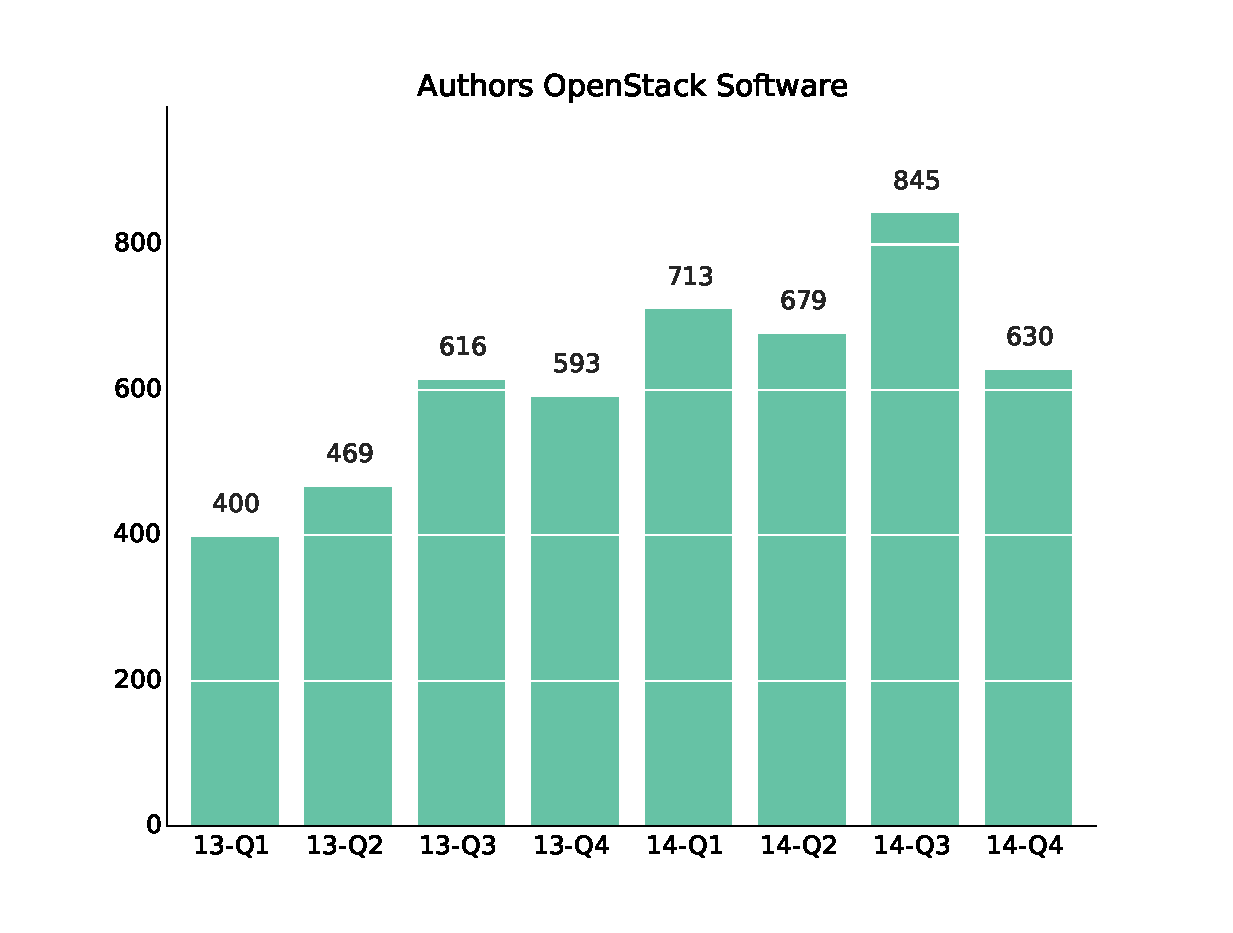
\includegraphics[scale=.35]{figs/authorsOpenStackSoftware.eps}
    & 
    \vspace{0pt}
    \begin{tabular}{l|l}%
    \bfseries Period & \bfseries Authors % specify table head
    \csvreader[head to column names]{data/authorsOpenStackSoftware.csv}{}% use head of csv as column names
    {\\\labels & \authors}
    \end{tabular}
\end{tabular}

\begin{tabular}{p{7cm} p{5cm}}
    \vspace{0pt}
\begin{tabular}{l|l}%
    \bfseries Commit (s) & \bfseries Author % specify table head
    \csvreader[head to column names]{data/scm_top_authors_project_OpenStackSoftware.csv}{}% use head of csv as column names
    {\\\hline\csvcoli&\csvcolii}% specify your coloumns here
\end{tabular}
&
\vspace{0pt}
\begin{tabular}{l|l}%
    \bfseries Commit (s) & \bfseries Organizations % specify table head
    \csvreader[head to column names]{data/scm_top_companies_project_OpenStackSoftware.csv}{}% use head of csv as column names
    {\\\hline\csvcoli&\csvcolii}% specify your coloumns here
\end{tabular}
\end {tabular}


\textbf{Process}: Efficiency closing changesets and tickets, time to review (mean and median), number of patchests (iterations)
per changeset and study on the time waiting for a reviewer or submitter action in the patchset review process.


\begin{tabular}{p{7cm} p{5cm}}
    \vspace{0pt} 
    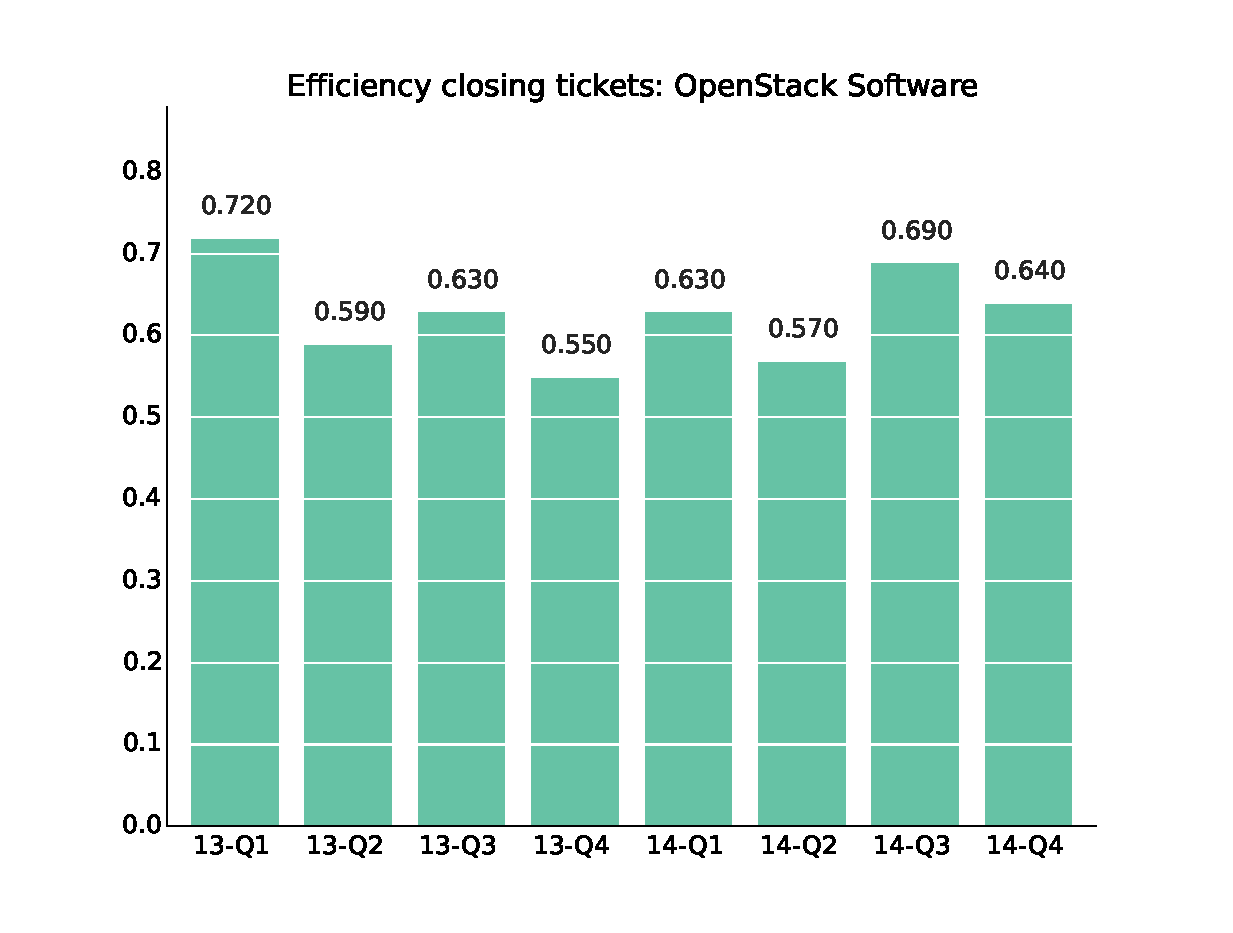
\includegraphics[scale=.35]{figs/bmiOpenStackSoftware.eps}
    & 
    \vspace{0pt}
    \begin{tabular}{l|l}%
    \bfseries Period & \bfseries Closed/Opened % specify table head
    \csvreader[head to column names]{data/bmiOpenStackSoftware.csv}{}% use head of csv as column names
    {\\\labels & \bmi}
    \end{tabular}
\end{tabular}

\begin{tabular}{p{7cm} p{5cm}}
    \vspace{0pt} 
    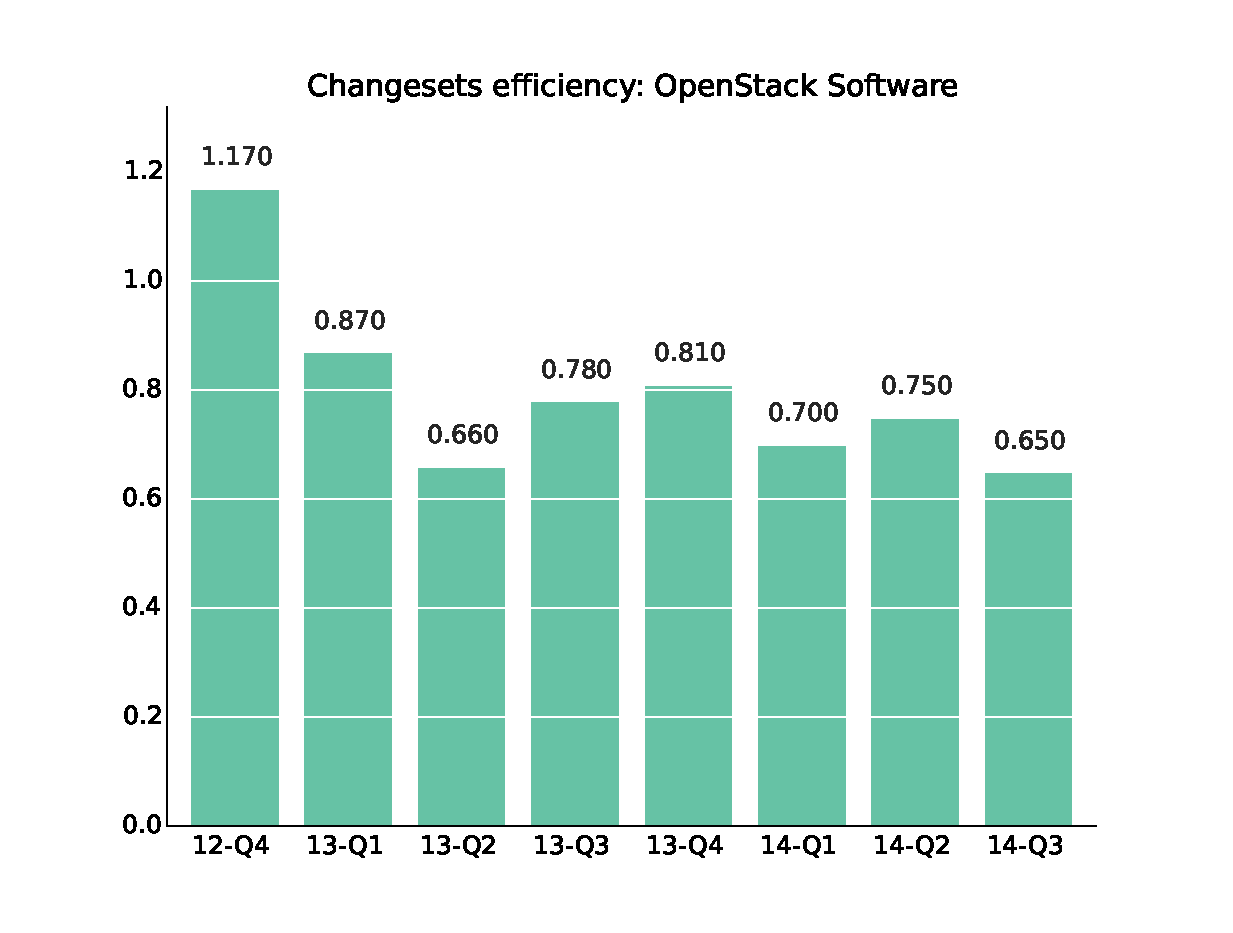
\includegraphics[scale=.35]{figs/bmiscrOpenStackSoftware.eps}
    & 
    \vspace{0pt}
    \begin{tabular}{l|l}%
    \bfseries Period & \bfseries (Aband. and Merg.)/Subm. % specify table head
    \csvreader[head to column names]{data/submitted_reviewsOpenStackSoftware.csv}{}% use head of csv as column names
    {\\\labels & \bmi}
    \end{tabular}
\end{tabular}


\begin{tabular}{p{7cm} p{5cm}}
    \vspace{0pt} 
    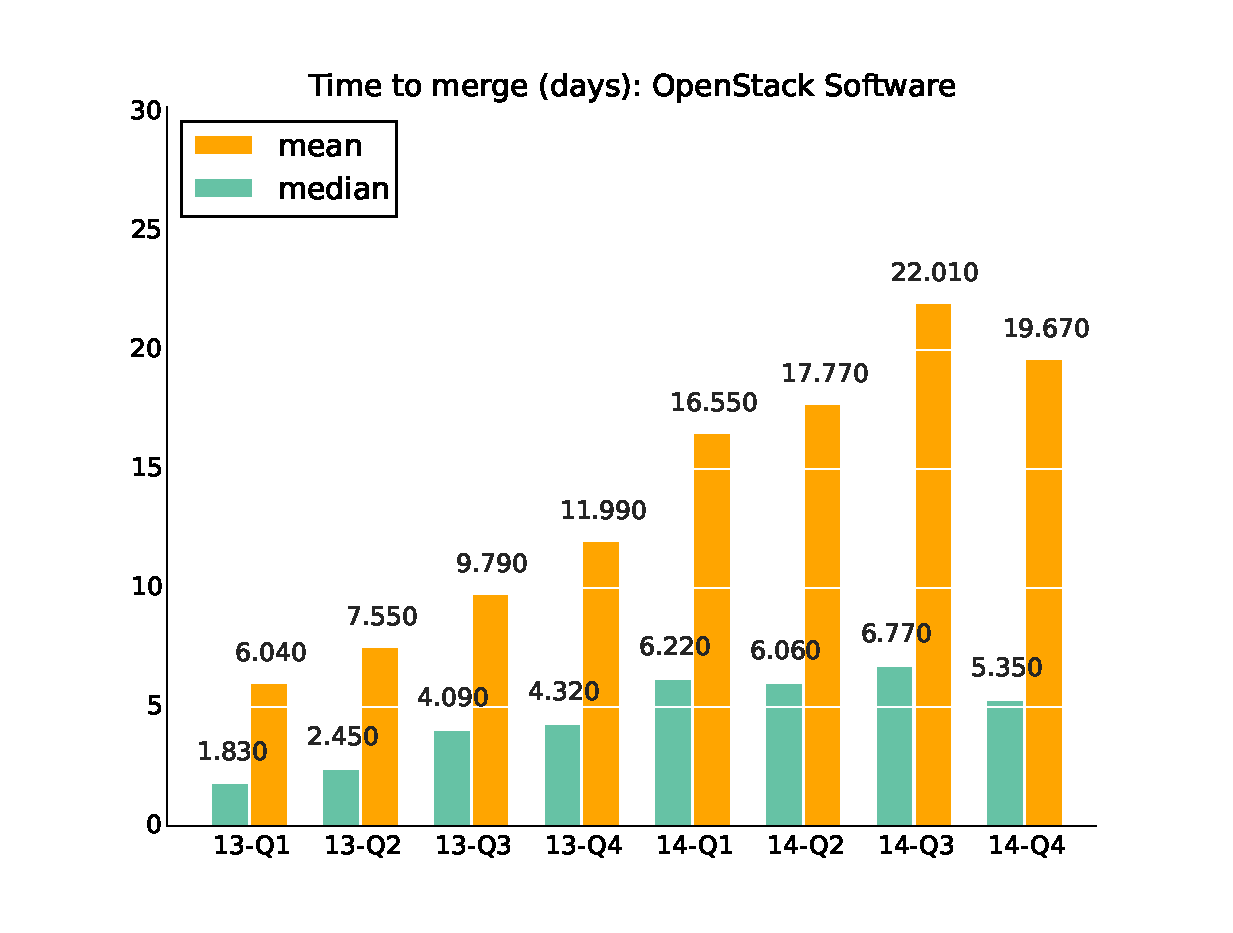
\includegraphics[scale=.35]{figs/timetoreview_medianOpenStackSoftware.eps}
    & 
    \vspace{0pt}
    \begin{tabular}{l|r|r|}%
    \bfseries Period & \bfseries Median & \bfseries Mean % specify table head
    \csvreader[head to column names]{data/timetoreview_medianOpenStackSoftware.csv}{}% use head of csv as column names
    {\\\labels & \mediantime & \meantime}
    \end{tabular}
\end{tabular}


\begin{tabular}{p{7cm} p{5cm}}
    \vspace{0pt} 
    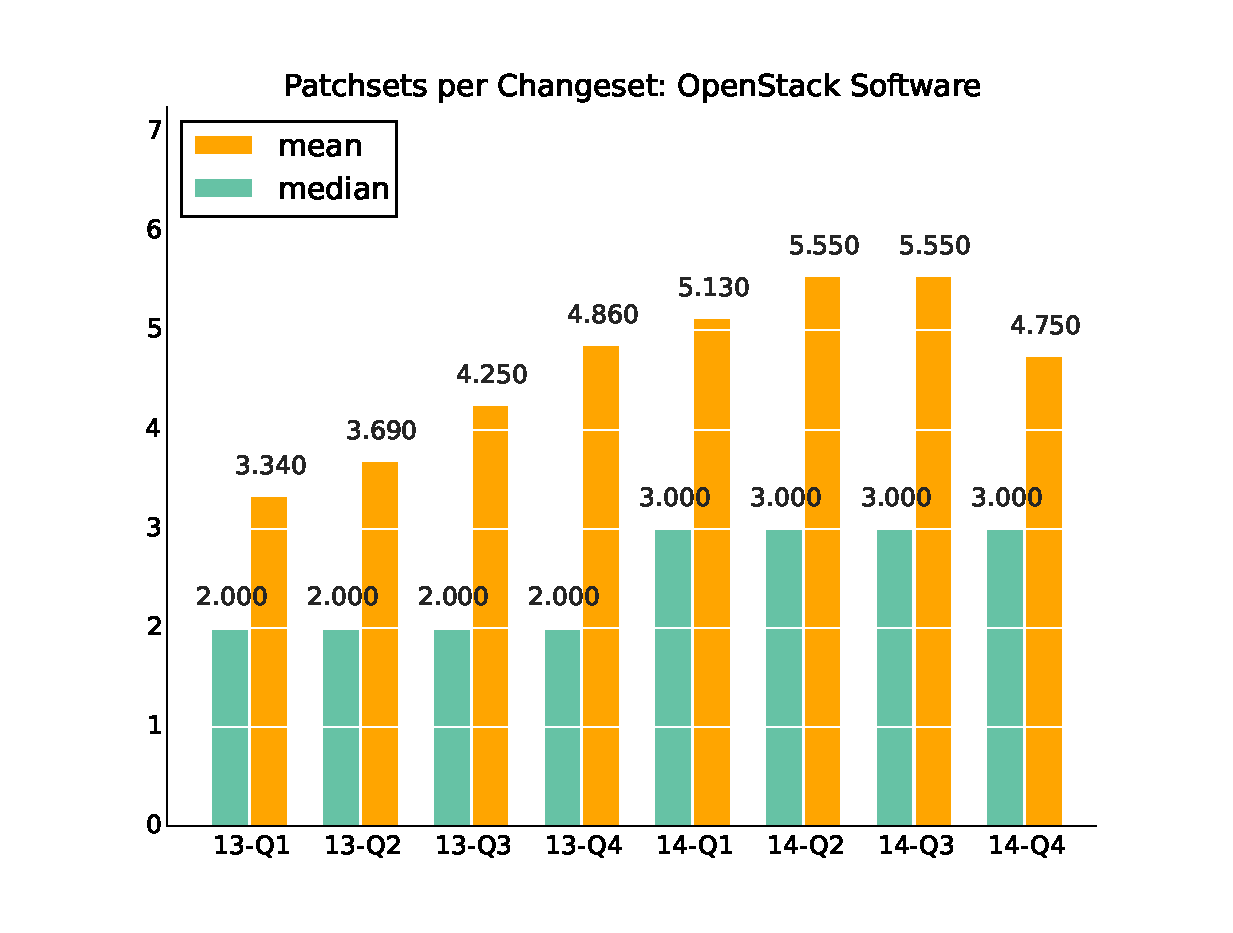
\includegraphics[scale=.35]{figs/patchsets_avgOpenStackSoftware.eps}
    & 
    \vspace{0pt}
    \begin{tabular}{l|r|r|}%
    \bfseries Period & \bfseries Median & \bfseries Mean % specify table head
    \csvreader[head to column names]{data/scr_patchsets_iterationsOpenStackSoftware.csv}{}% use head of csv as column names
    {\\\labels & \medianpatchsets & \meanpatchsets}
    \end{tabular}
\end{tabular}

\begin{tabular}{p{7cm} p{5cm}}
    \vspace{0pt} 
    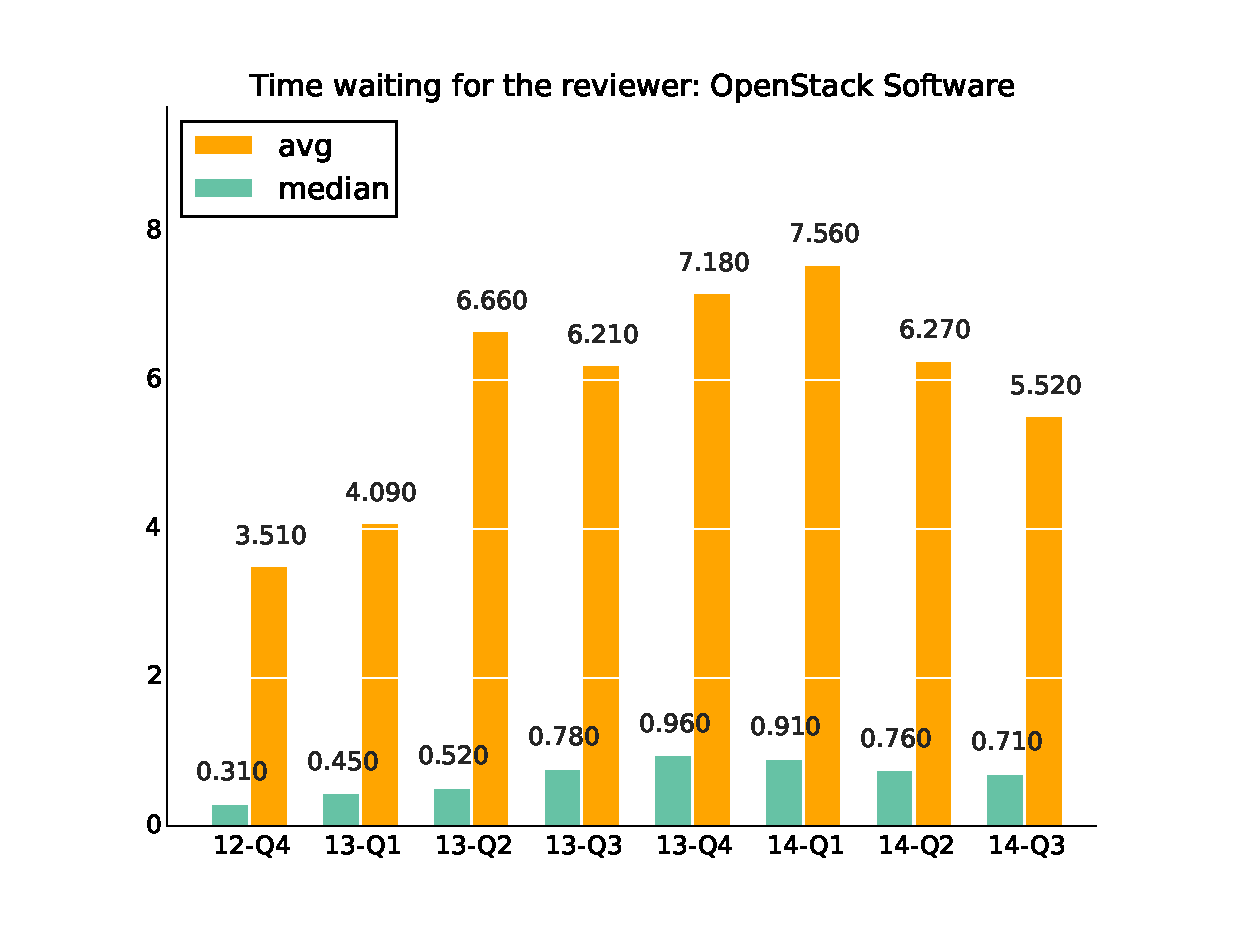
\includegraphics[scale=.35]{figs/waiting4reviewer_avgOpenStackSoftware.eps}
    & 
    \vspace{0pt}
    \begin{tabular}{l|r|r|}%
    \bfseries Period & \bfseries Median & \bfseries Mean % specify table head
    \csvreader[head to column names]{data/timewaiting4reviewer_medianOpenStackSoftware.csv}{}% use head of csv as column names
    {\\\labels & \mediantime & \meantime}
    \end{tabular}
\end{tabular}

\begin{tabular}{p{7cm} p{5cm}}
    \vspace{0pt} 
    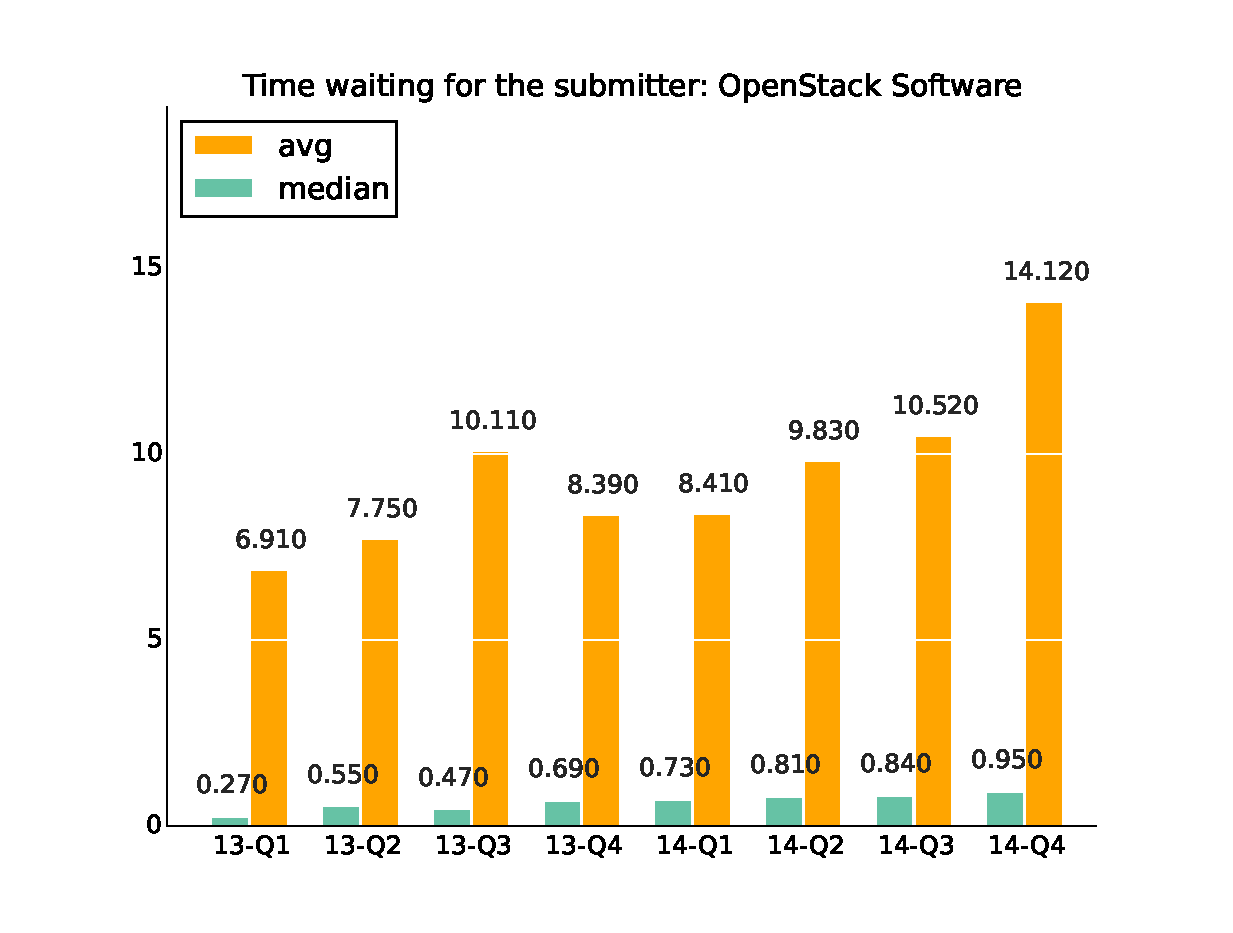
\includegraphics[scale=.35]{figs/waiting4submitter_avgOpenStackSoftware.eps}
    & 
    \vspace{0pt}
    \begin{tabular}{l|r|r|}%
    \bfseries Period & \bfseries Median & \bfseries Mean % specify table head
    \csvreader[head to column names]{data/timewaiting4submitter_medianOpenStackSoftware.csv}{}% use head of csv as column names
    {\\\labels & \mediantime & \meantime}
    \end{tabular}
\end{tabular}



\newpage
\subsection{OpenStack Integrated Programs}
\textbf{Activity}: Commits in Git, submitted, merged and abandoned reviews in Gerrit and opened and closed issues in Launchpad.


\begin{tabular}{p{7cm} p{5cm}}
    \vspace{0pt} 
    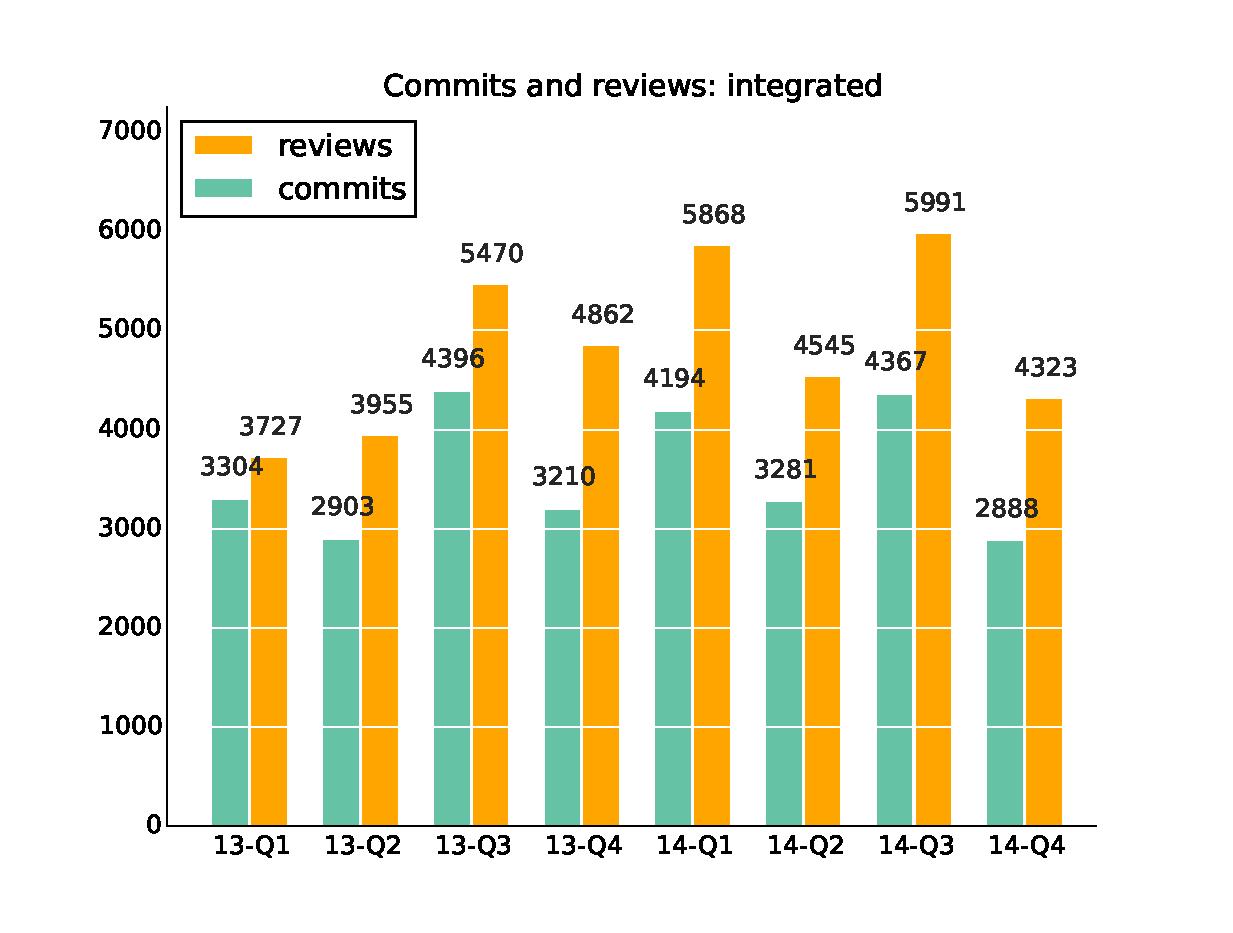
\includegraphics[scale=.35]{figs/commitsintegrated.eps}
    & 
    \vspace{0pt}
    \begin{tabular}{l|r|r|}%
    \bfseries Period & \bfseries Commits & \bfseries Reviews% specify table head
    \csvreader[head to column names]{data/commitsintegrated.csv}{}% use head of csv as column names
    {\\\labels & \commits & \submitted}
    \end{tabular}
\end{tabular}

\begin{tabular}{p{7cm} p{5cm}}
    \vspace{0pt} 
    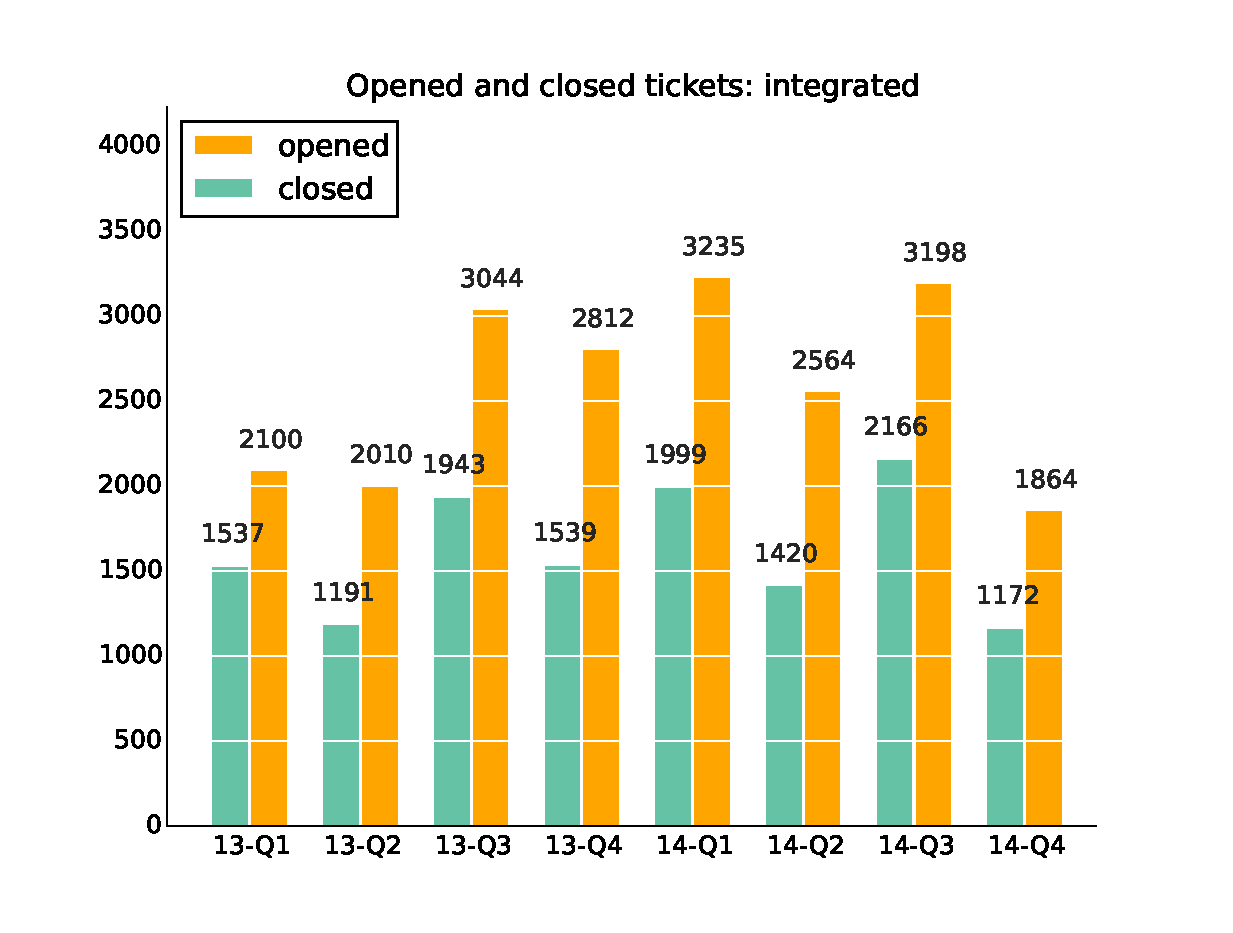
\includegraphics[scale=.35]{figs/closedintegrated.eps}
    & 
    \vspace{0pt}
    \begin{tabular}{l|r|r|}%
    \bfseries Period & \bfseries Closed & \bfseries Opened% specify table head
    \csvreader[head to column names]{data/closedintegrated.csv}{}% use head of csv as column names
    {\\\labels & \closed & \opened}
    \end{tabular}
\end{tabular}

\begin{tabular}{p{7cm} p{5cm}}
    \vspace{0pt} 
    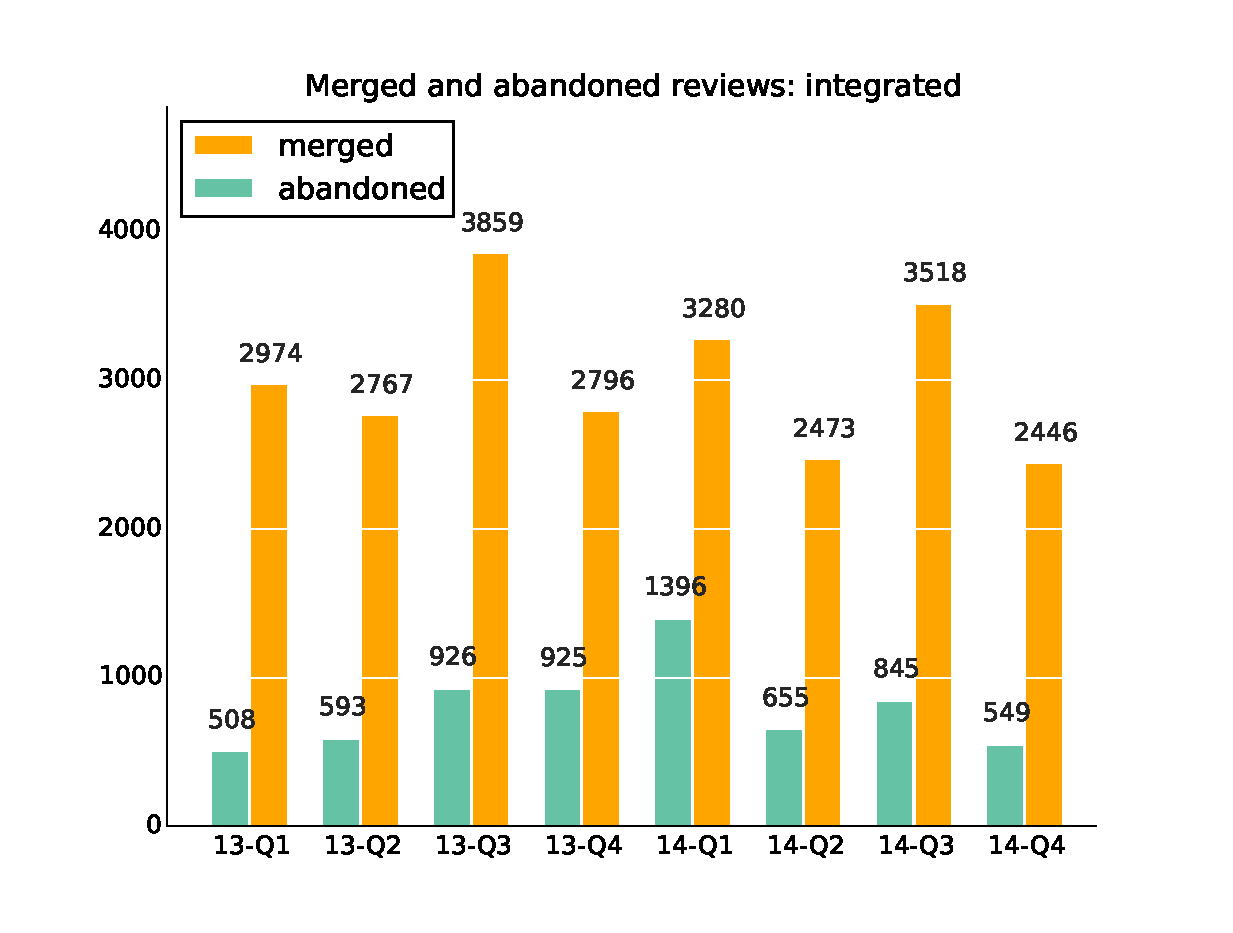
\includegraphics[scale=.35]{figs/submitted_reviewsintegrated.eps}
    & 
    \vspace{0pt}
    \begin{tabular}{l|r|r|}%
    \bfseries Period & \bfseries Merged & \bfseries Abandoned % specify table head
    \csvreader[head to column names]{data/submitted_reviewsintegrated.csv}{}% use head of csv as column names
    {\\\labels & \merged & \abandoned}
    \end{tabular}
\end{tabular}


\section{Community}
Active core reviewers in Gerrit, active authors in Git, top authors and organizations in the last quarter


\begin{tabular}{p{7cm} p{5cm}}
    \vspace{0pt} 
    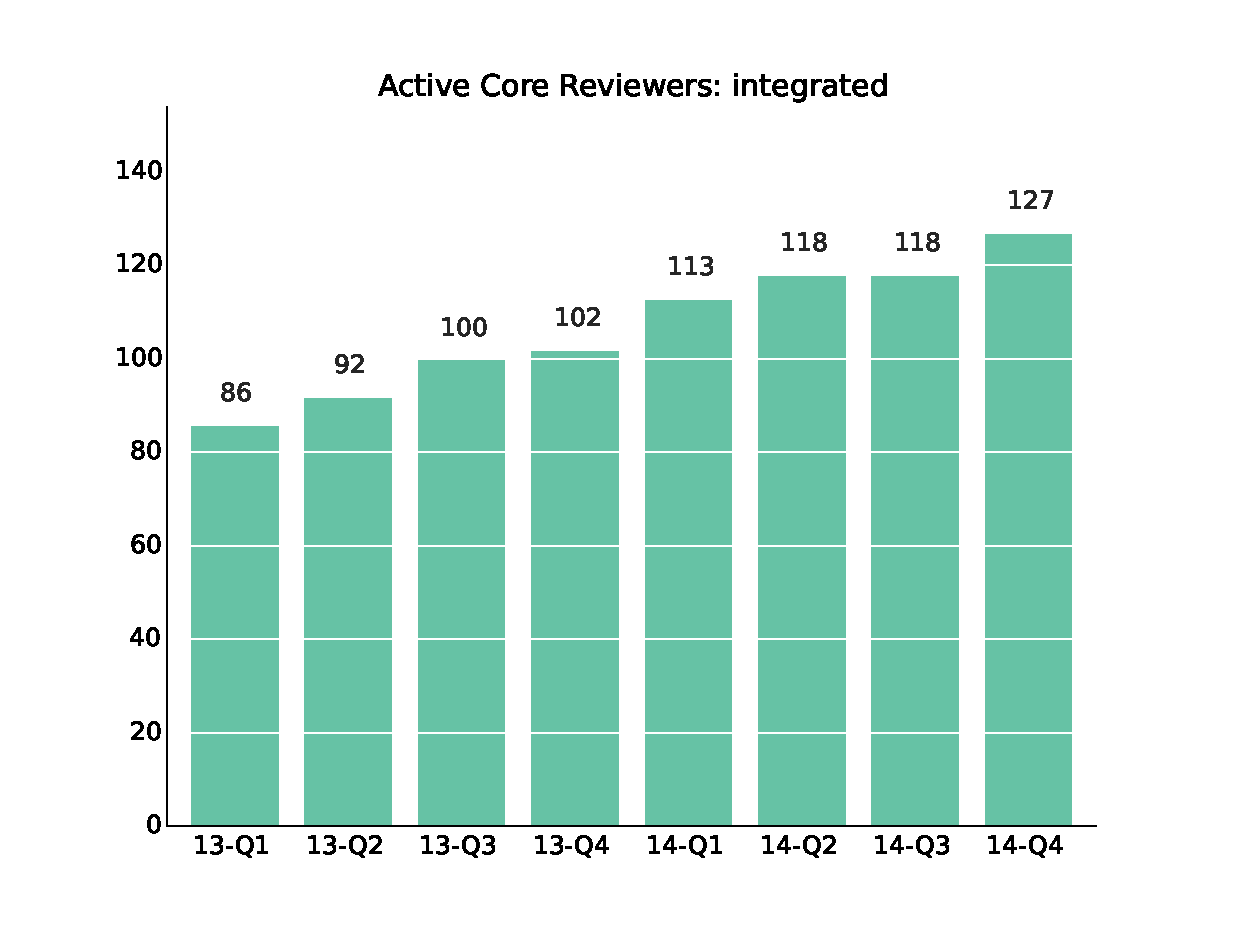
\includegraphics[scale=.35]{figs/active_core_scrintegrated.eps}
    & 
    \vspace{0pt}
    \begin{tabular}{l|l}%
    \bfseries Period & \bfseries Active Core % specify table head
    \csvreader[head to column names]{data/active_core_scrintegrated.csv}{}% use head of csv as column names
    {\\\labels & \activecorereviewers}
    \end{tabular}
\end{tabular}

\begin{tabular}{p{7cm} p{5cm}}
    \vspace{0pt} 
    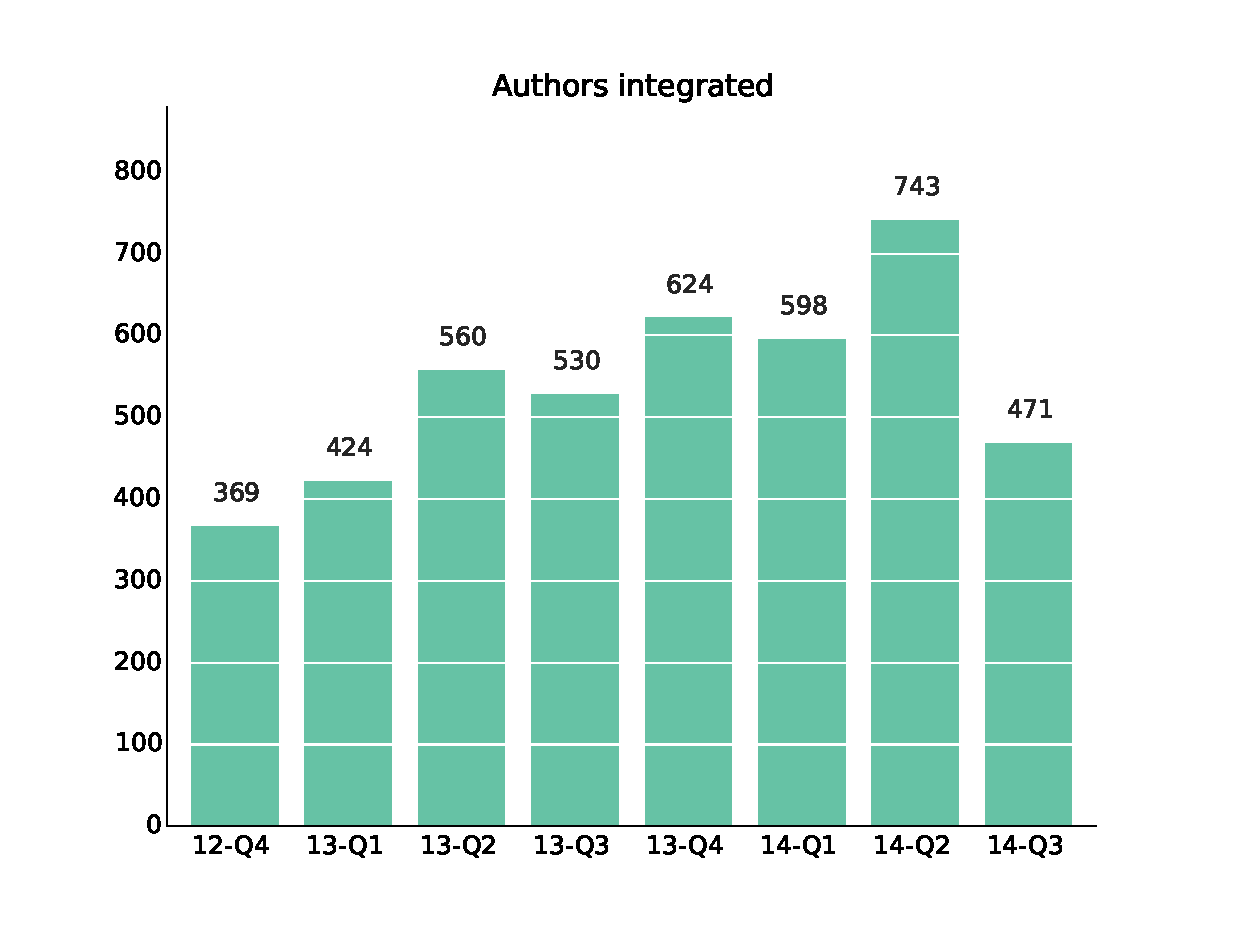
\includegraphics[scale=.35]{figs/authorsintegrated.eps}
    & 
    \vspace{0pt}
    \begin{tabular}{l|l}%
    \bfseries Period & \bfseries Authors % specify table head
    \csvreader[head to column names]{data/authorsintegrated.csv}{}% use head of csv as column names
    {\\\labels & \authors}
    \end{tabular}
\end{tabular}

\begin{tabular}{p{7cm} p{5cm}}
    \vspace{0pt}
\begin{tabular}{l|l}%
    \bfseries Commit (s) & \bfseries Author % specify table head
    \csvreader[head to column names]{data/scm_top_authors_project_integrated.csv}{}% use head of csv as column names
    {\\\hline\csvcoli&\csvcolii}% specify your coloumns here
\end{tabular}
&
\vspace{0pt}
\begin{tabular}{l|l}%
    \bfseries Commit (s) & \bfseries Organizations % specify table head
    \csvreader[head to column names]{data/scm_top_companies_project_integrated.csv}{}% use head of csv as column names
    {\\\hline\csvcoli&\csvcolii}% specify your coloumns here
\end{tabular}
\end {tabular}


\textbf{Process}: Efficiency closing changesets and tickets, time to review (mean and median), number of patchests (iterations)
per changeset and study on the time waiting for a reviewer or submitter action in the patchset review process.


\begin{tabular}{p{7cm} p{5cm}}
    \vspace{0pt} 
    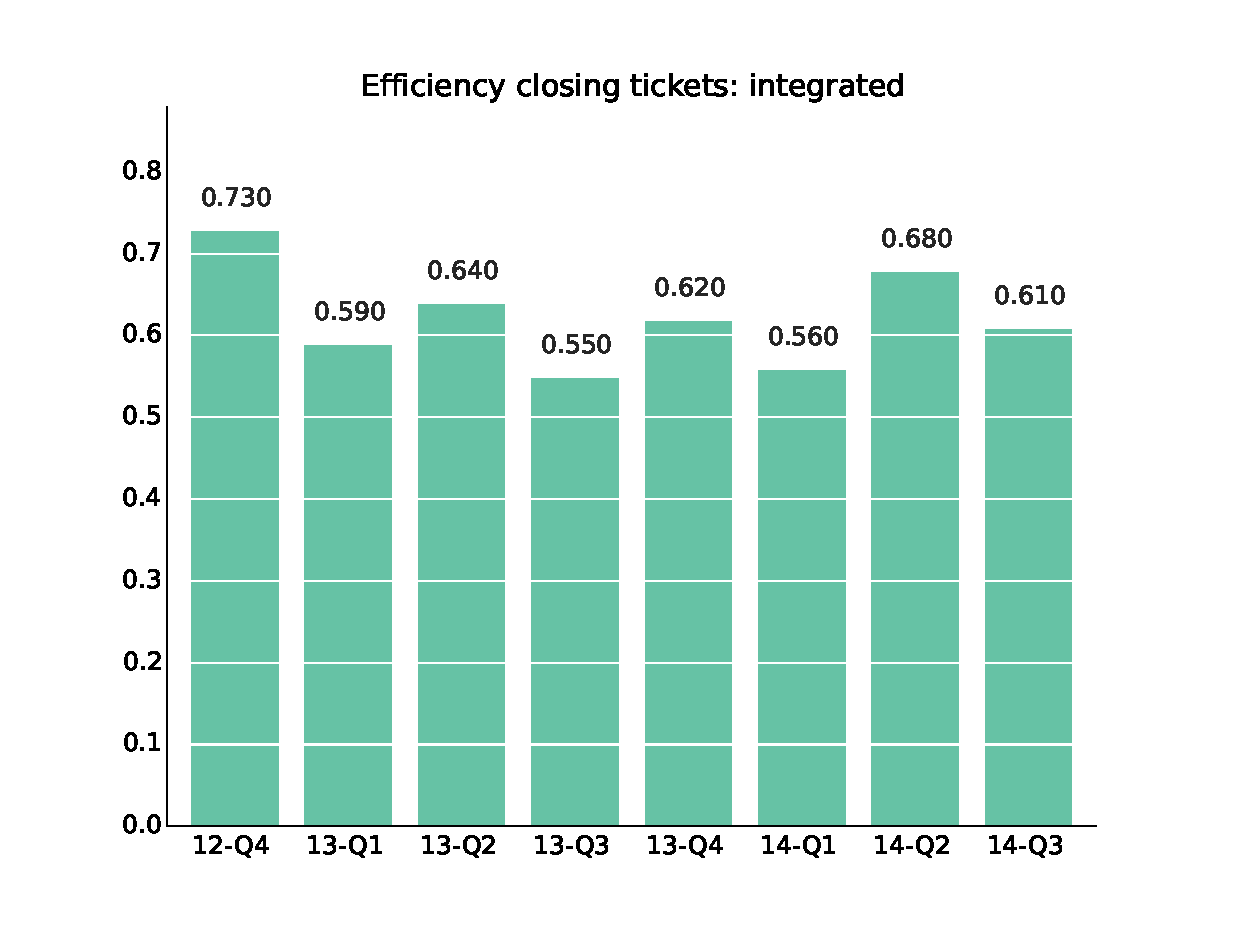
\includegraphics[scale=.35]{figs/bmiintegrated.eps}
    & 
    \vspace{0pt}
    \begin{tabular}{l|l}%
    \bfseries Period & \bfseries Closed/Opened % specify table head
    \csvreader[head to column names]{data/bmiintegrated.csv}{}% use head of csv as column names
    {\\\labels & \bmi}
    \end{tabular}
\end{tabular}

\begin{tabular}{p{7cm} p{5cm}}
    \vspace{0pt} 
    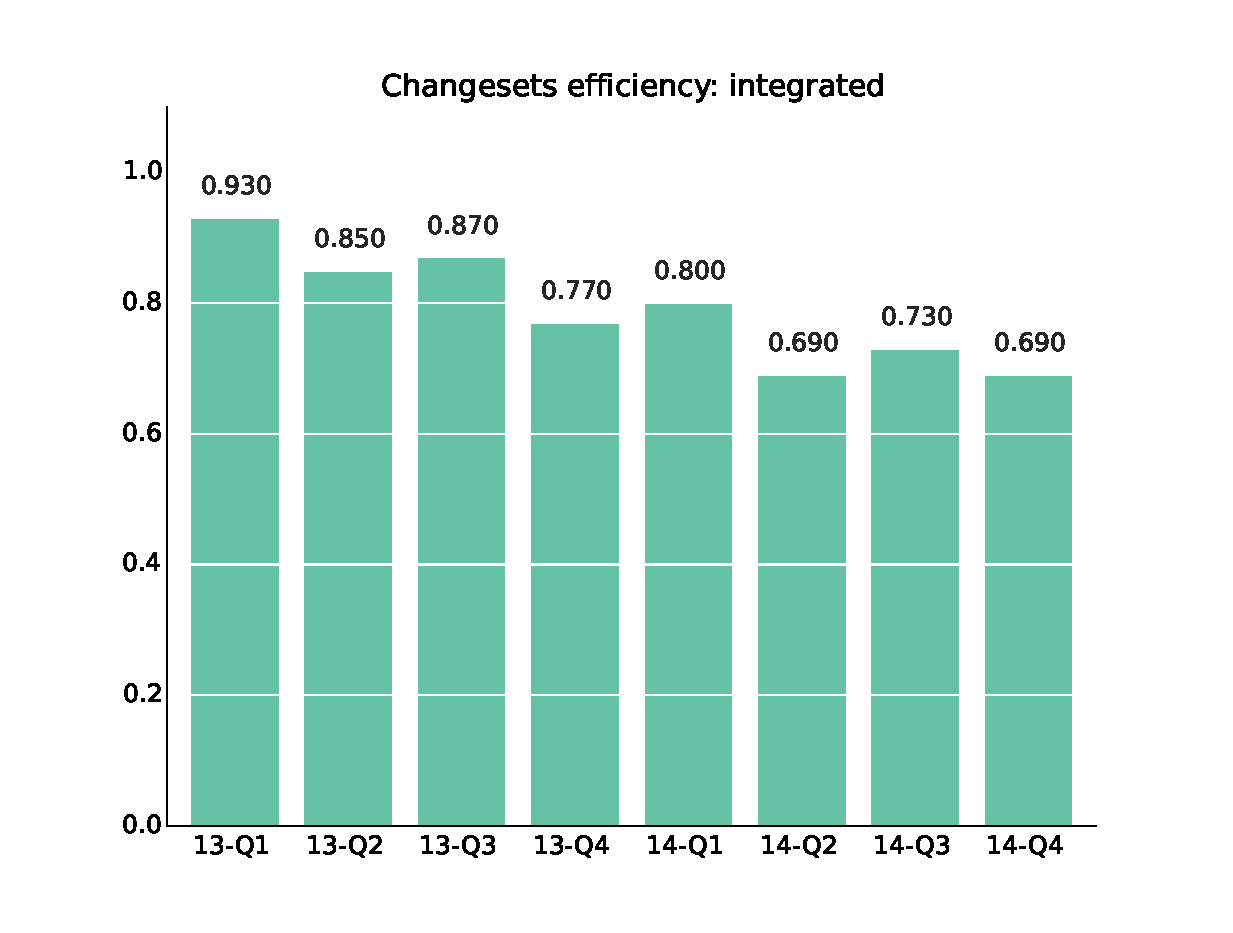
\includegraphics[scale=.35]{figs/bmiscrintegrated.eps}
    & 
    \vspace{0pt}
    \begin{tabular}{l|l}%
    \bfseries Period & \bfseries (Aband. and Merg.)/Subm. % specify table head
    \csvreader[head to column names]{data/submitted_reviewsintegrated.csv}{}% use head of csv as column names
    {\\\labels & \bmi}
    \end{tabular}
\end{tabular}


\begin{tabular}{p{7cm} p{5cm}}
    \vspace{0pt} 
    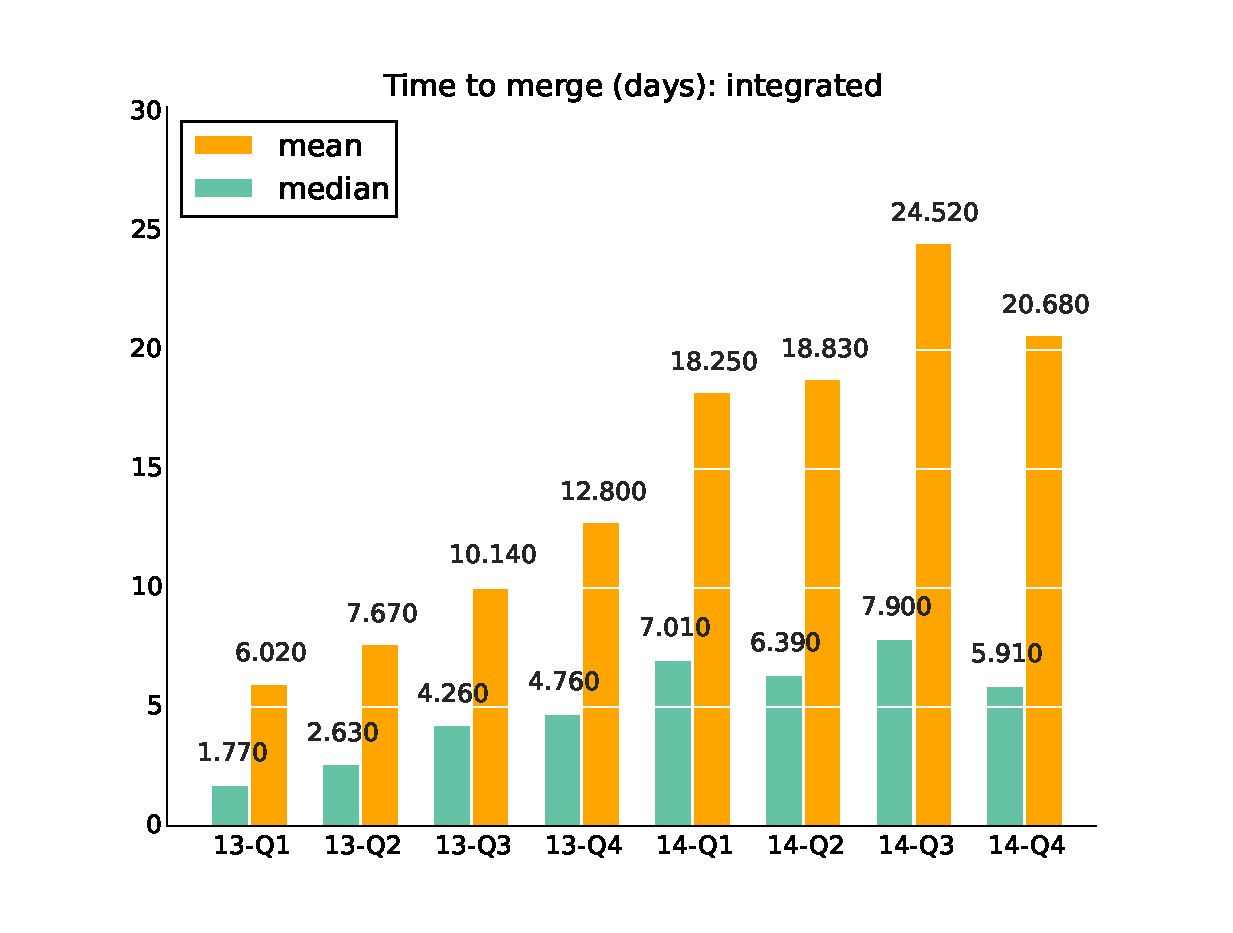
\includegraphics[scale=.35]{figs/timetoreview_medianintegrated.eps}
    & 
    \vspace{0pt}
    \begin{tabular}{l|r|r|}%
    \bfseries Period & \bfseries Median & \bfseries Mean % specify table head
    \csvreader[head to column names]{data/timetoreview_medianintegrated.csv}{}% use head of csv as column names
    {\\\labels & \mediantime & \meantime}
    \end{tabular}
\end{tabular}


\begin{tabular}{p{7cm} p{5cm}}
    \vspace{0pt} 
    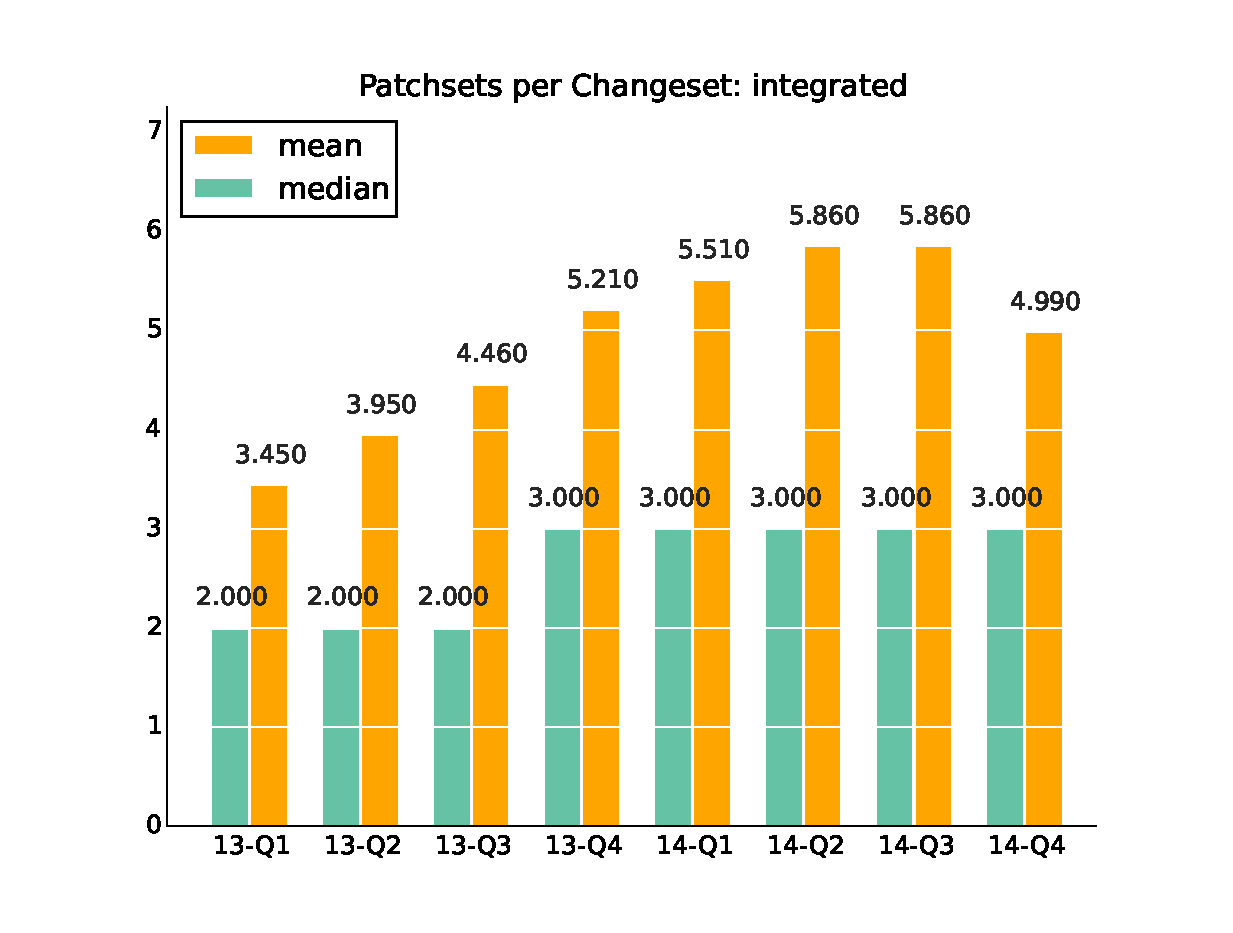
\includegraphics[scale=.35]{figs/patchsets_avgintegrated.eps}
    & 
    \vspace{0pt}
    \begin{tabular}{l|r|r|}%
    \bfseries Period & \bfseries Median & \bfseries Mean % specify table head
    \csvreader[head to column names]{data/scr_patchsets_iterationsintegrated.csv}{}% use head of csv as column names
    {\\\labels & \medianpatchsets & \meanpatchsets}
    \end{tabular}
\end{tabular}

\begin{tabular}{p{7cm} p{5cm}}
    \vspace{0pt} 
    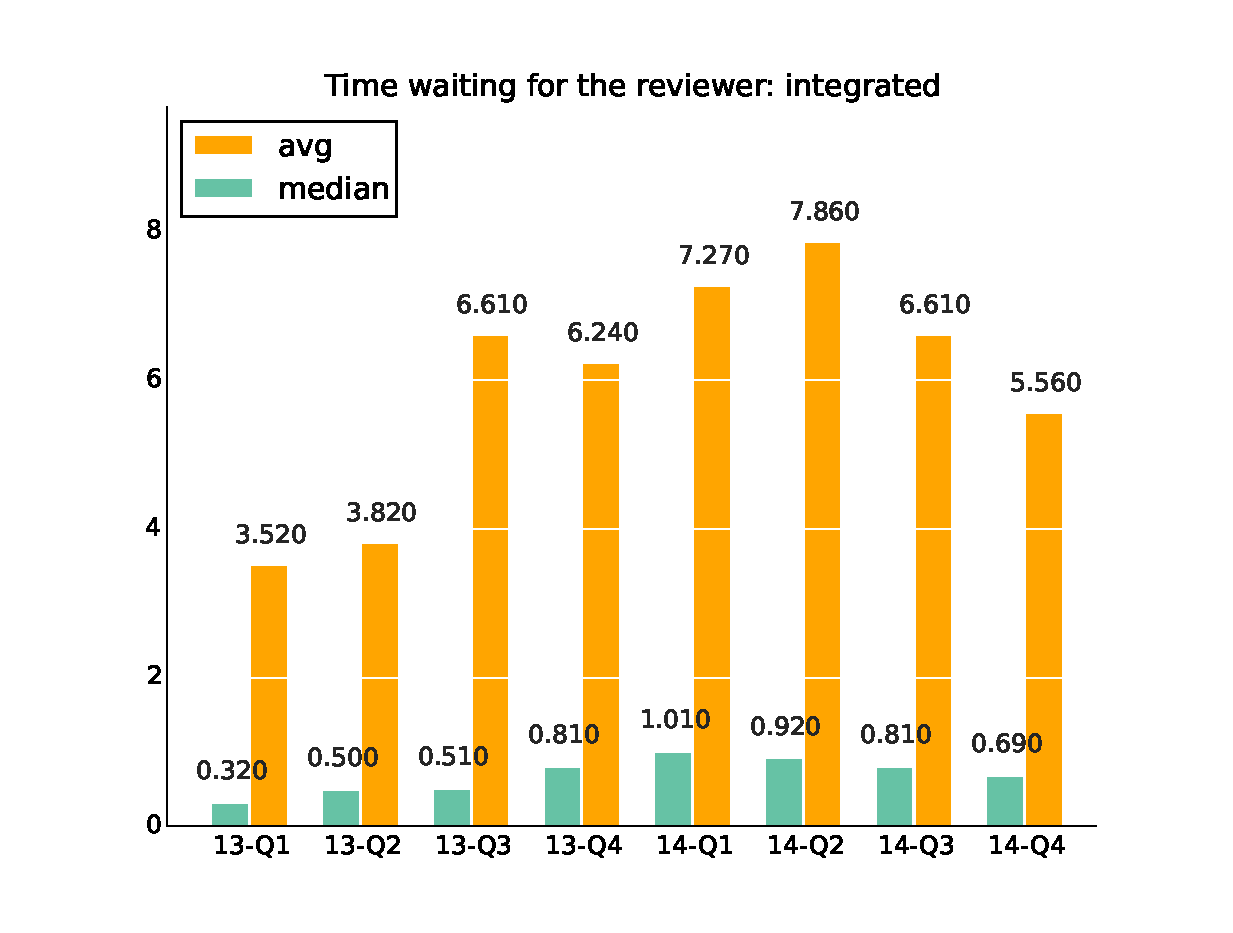
\includegraphics[scale=.35]{figs/waiting4reviewer_avgintegrated.eps}
    & 
    \vspace{0pt}
    \begin{tabular}{l|r|r|}%
    \bfseries Period & \bfseries Median & \bfseries Mean % specify table head
    \csvreader[head to column names]{data/timewaiting4reviewer_medianintegrated.csv}{}% use head of csv as column names
    {\\\labels & \mediantime & \meantime}
    \end{tabular}
\end{tabular}

\begin{tabular}{p{7cm} p{5cm}}
    \vspace{0pt} 
    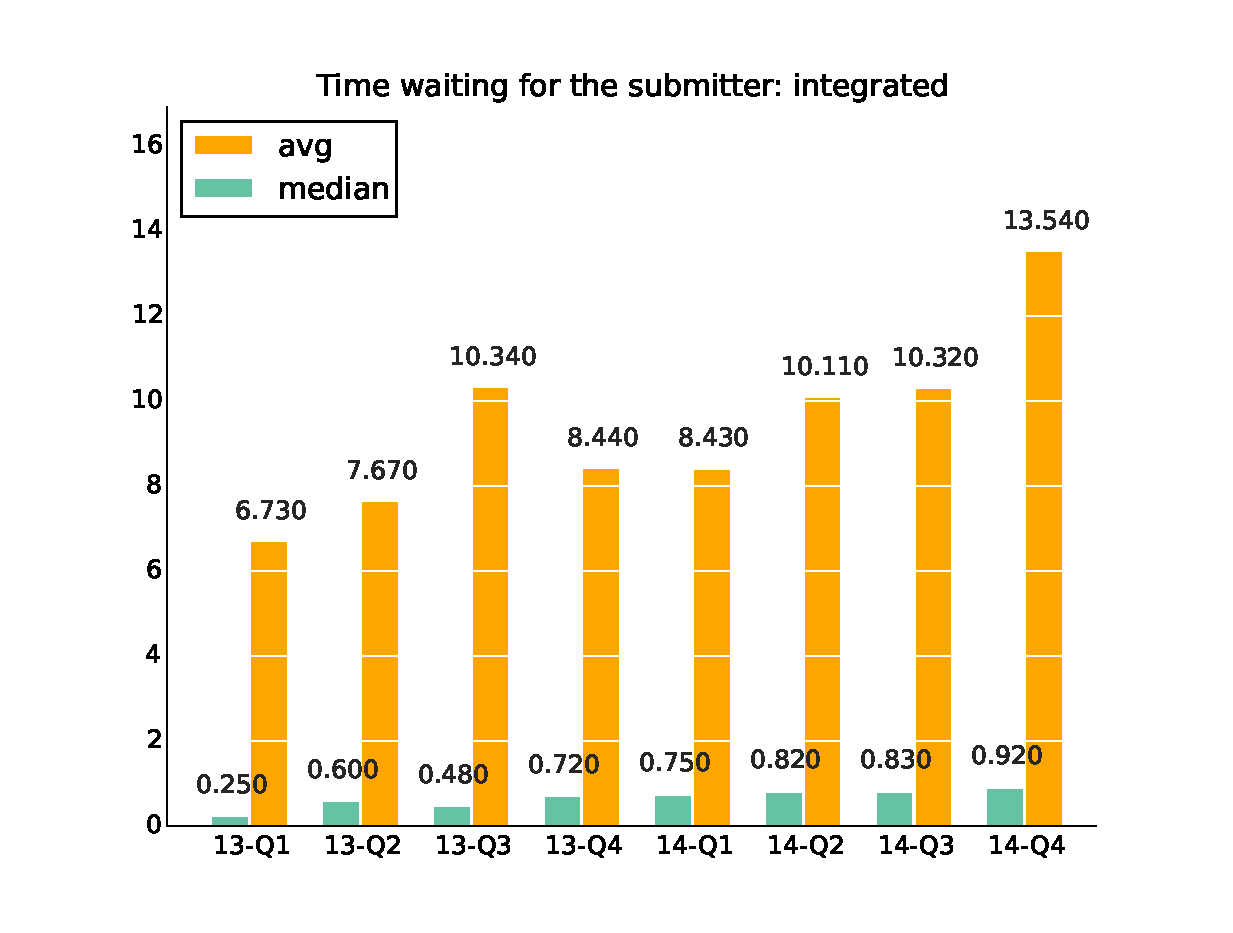
\includegraphics[scale=.35]{figs/waiting4submitter_avgintegrated.eps}
    & 
    \vspace{0pt}
    \begin{tabular}{l|r|r|}%
    \bfseries Period & \bfseries Median & \bfseries Mean % specify table head
    \csvreader[head to column names]{data/timewaiting4submitter_medianintegrated.csv}{}% use head of csv as column names
    {\\\labels & \mediantime & \meantime}
    \end{tabular}
\end{tabular}


\newpage
\subsection{Incubated}
\textbf{Activity}: Commits in Git, submitted, merged and abandoned reviews in Gerrit and opened and closed issues in Launchpad.


\begin{tabular}{p{7cm} p{5cm}}
    \vspace{0pt} 
    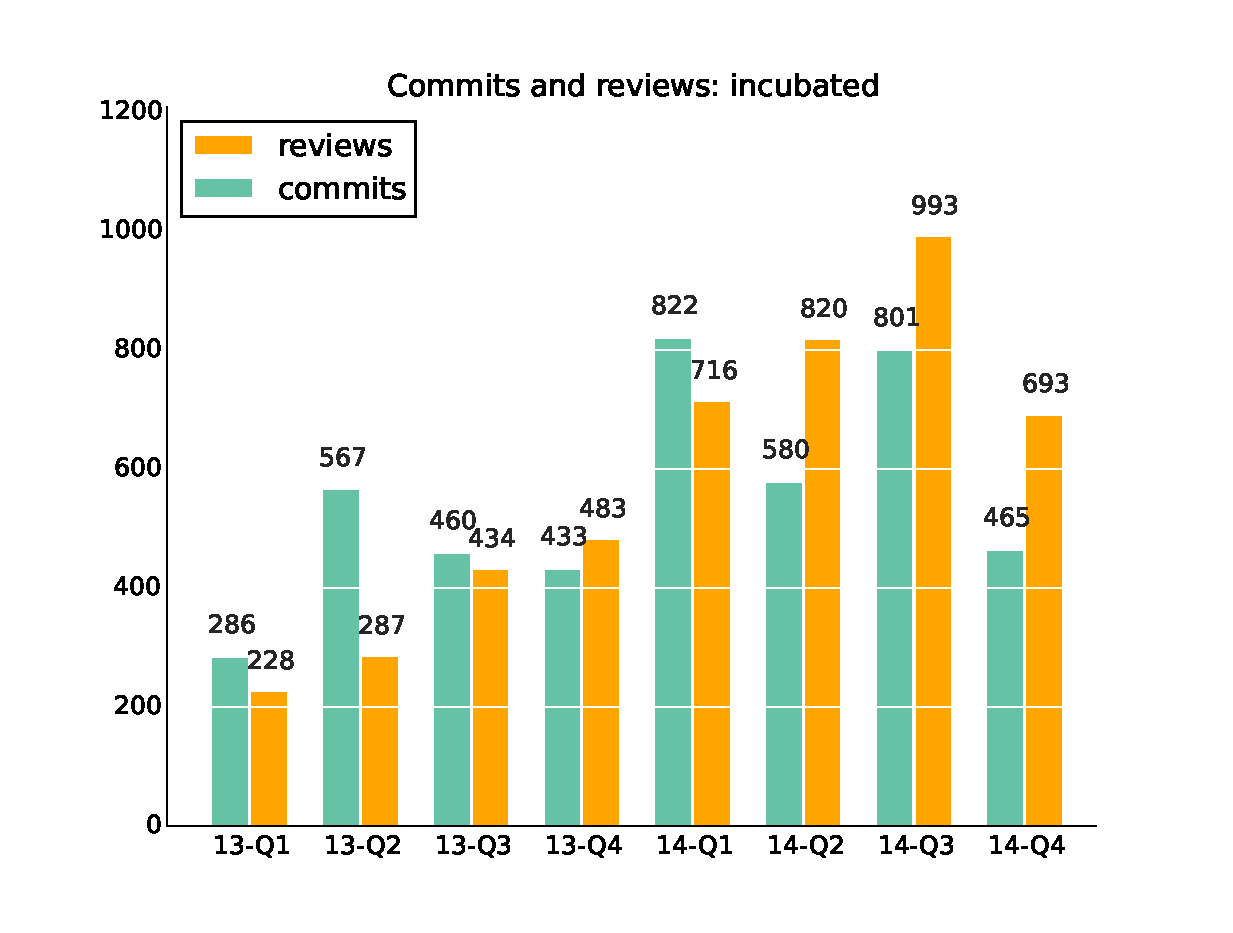
\includegraphics[scale=.35]{figs/commitsincubated.eps}
    & 
    \vspace{0pt}
    \begin{tabular}{l|r|r|}%
    \bfseries Period & \bfseries Commits & \bfseries Reviews % specify table head
    \csvreader[head to column names]{data/commitsincubated.csv}{}% use head of csv as column names
    {\\\labels & \commits & \submitted}
    \end{tabular}
\end{tabular}

\begin{tabular}{p{7cm} p{5cm}}
    \vspace{0pt} 
    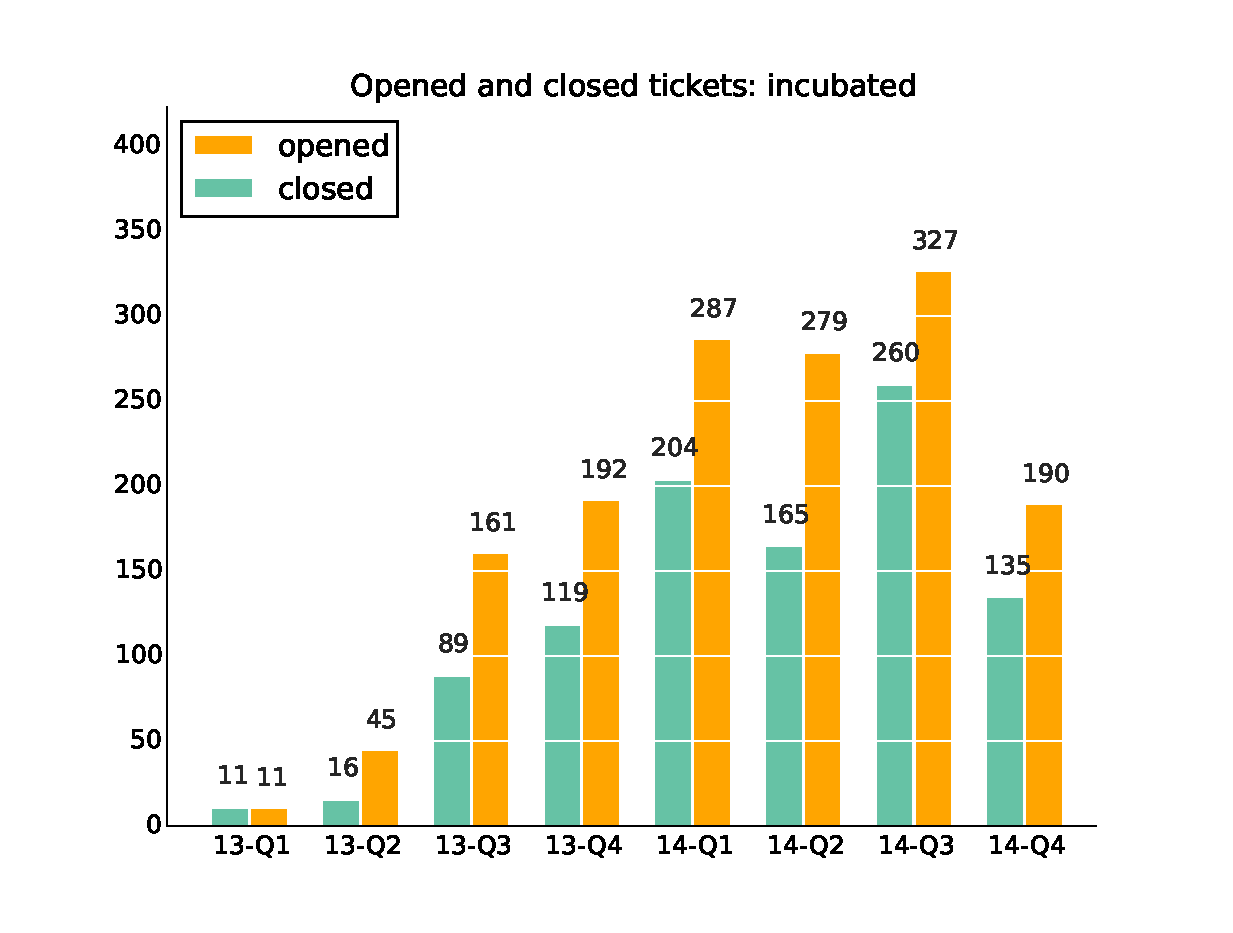
\includegraphics[scale=.35]{figs/closedincubated.eps}
    & 
    \vspace{0pt}
    \begin{tabular}{l|r|r|}%
\bfseries Period & \bfseries Closed & \bfseries Opened
    \csvreader[head to column names]{data/closedincubated.csv}{}% use head of csv as column names
    {\\\labels & \closed & \opened}
    \end{tabular}
\end{tabular}

\begin{tabular}{p{7cm} p{5cm}}
    \vspace{0pt} 
    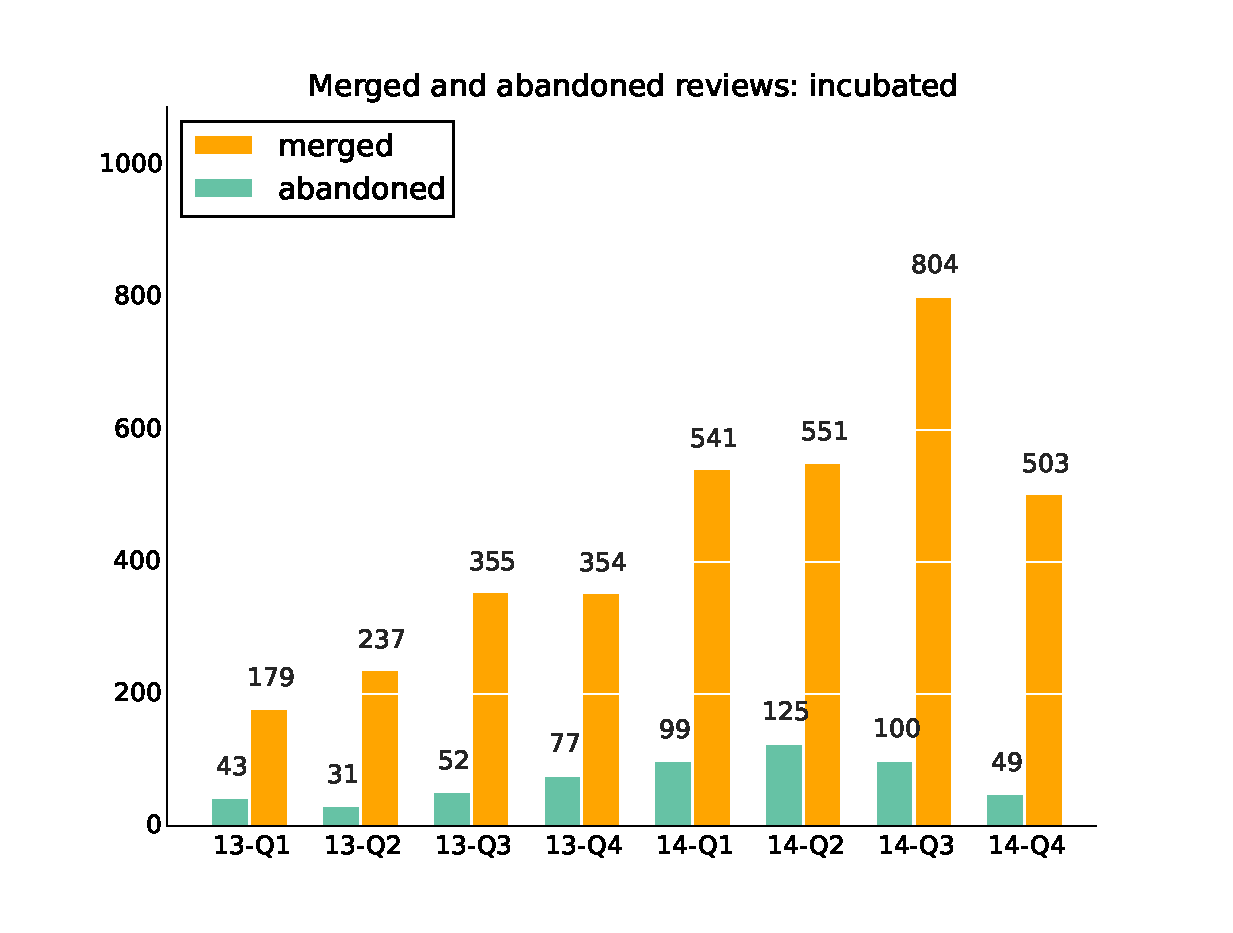
\includegraphics[scale=.35]{figs/submitted_reviewsincubated.eps}
    & 
    \vspace{0pt}
    \begin{tabular}{l|r|r|}%
    \bfseries Period & \bfseries Merged & \bfseries Abandoned % specify table head
    \csvreader[head to column names]{data/submitted_reviewsincubated.csv}{}% use head of csv as column names
    {\\\labels & \merged & \abandoned}
    \end{tabular}
\end{tabular}


\section{Community}
Active core reviewers in Gerrit, active authors in Git, top authors and organizations in the last quarter


\begin{tabular}{p{7cm} p{5cm}}
    \vspace{0pt} 
    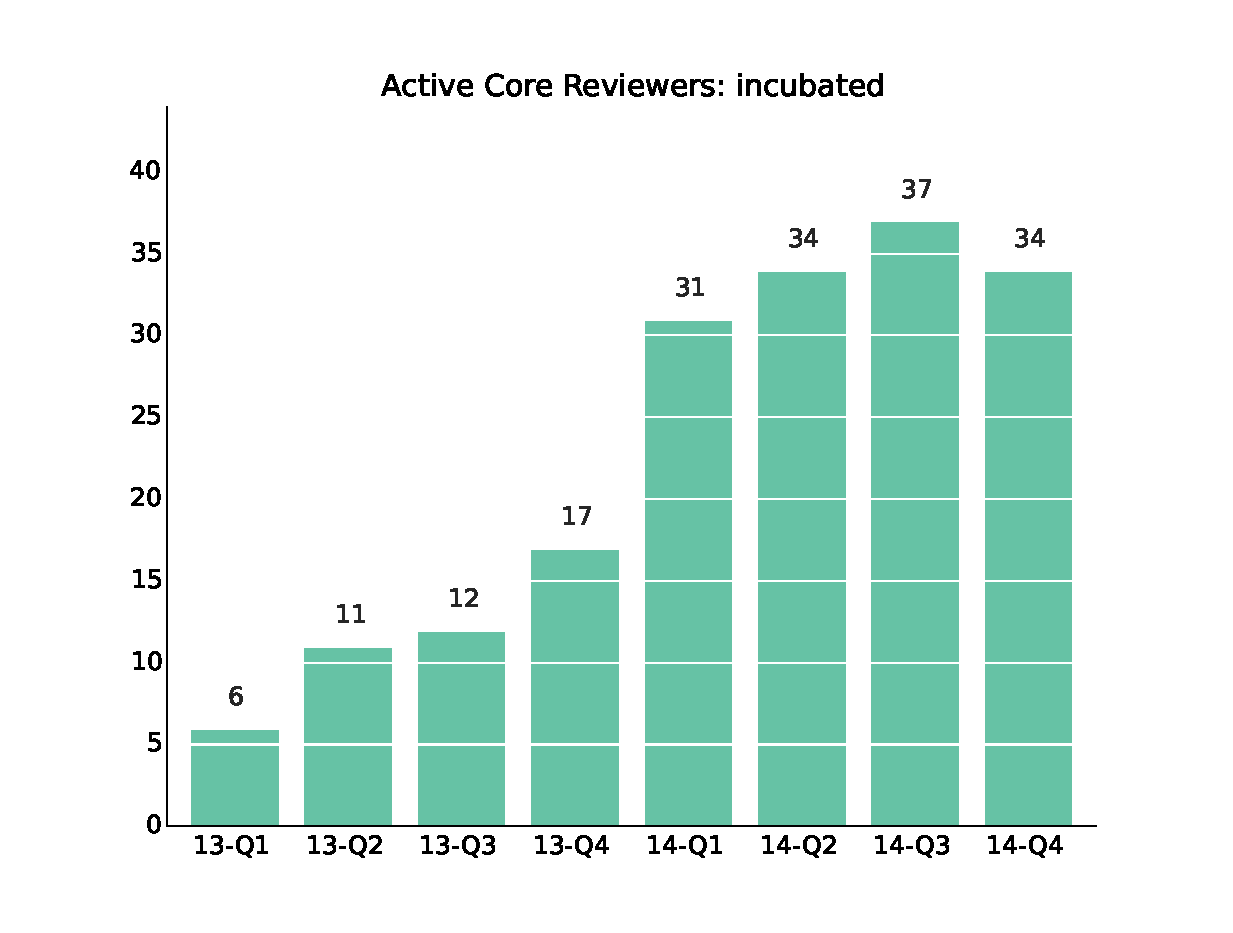
\includegraphics[scale=.35]{figs/active_core_scrincubated.eps}
    & 
    \vspace{0pt}
    \begin{tabular}{l|l}%
    \bfseries Period & \bfseries Active Core % specify table head
    \csvreader[head to column names]{data/active_core_scrincubated.csv}{}% use head of csv as column names
    {\\\labels & \activecorereviewers}
    \end{tabular}
\end{tabular}

\begin{tabular}{p{7cm} p{5cm}}
    \vspace{0pt} 
    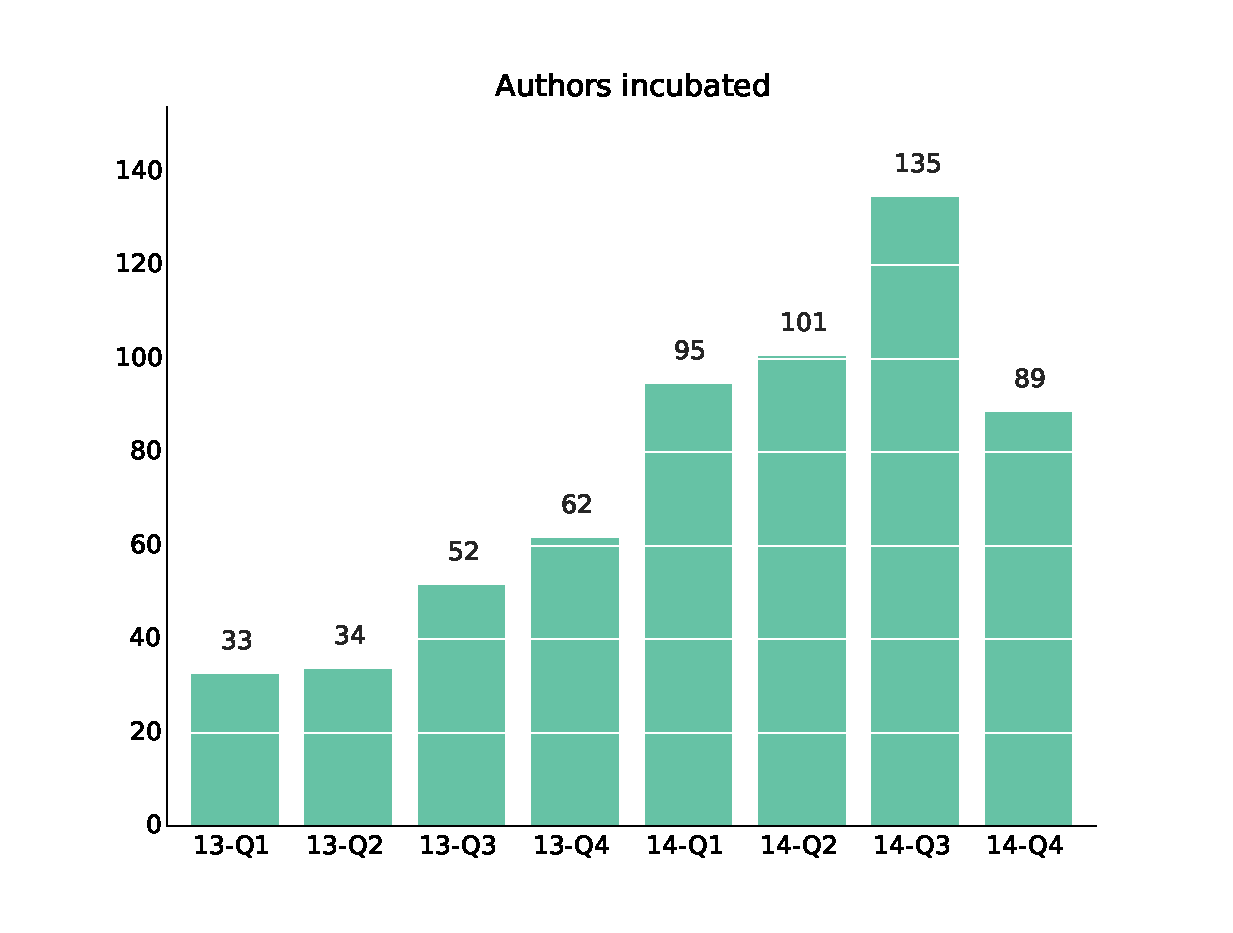
\includegraphics[scale=.35]{figs/authorsincubated.eps}
    & 
    \vspace{0pt}
    \begin{tabular}{l|l}%
    \bfseries Period & \bfseries Authors % specify table head
    \csvreader[head to column names]{data/authorsincubated.csv}{}% use head of csv as column names
    {\\\labels & \authors}
    \end{tabular}
\end{tabular}

\begin{tabular}{p{7cm} p{5cm}}
    \vspace{0pt}
\begin{tabular}{l|l}%
    \bfseries Commit (s) & \bfseries Author % specify table head
    \csvreader[head to column names]{data/scm_top_authors_project_incubated.csv}{}% use head of csv as column names
    {\\\hline\csvcoli&\csvcolii}% specify your coloumns here
\end{tabular}
&
\vspace{0pt}
\begin{tabular}{l|l}%
    \bfseries Commit (s) & \bfseries Organizations % specify table head
    \csvreader[head to column names]{data/scm_top_companies_project_incubated.csv}{}% use head of csv as column names
    {\\\hline\csvcoli&\csvcolii}% specify your coloumns here
\end{tabular}
\end {tabular}

\textbf{Process}: Efficiency closing changesets and tickets, time to review (mean and median), number of patchests (iterations)
per changeset and study on the time waiting for a reviewer or submitter action in the patchset review process.




\begin{tabular}{p{7cm} p{5cm}}
    \vspace{0pt} 
    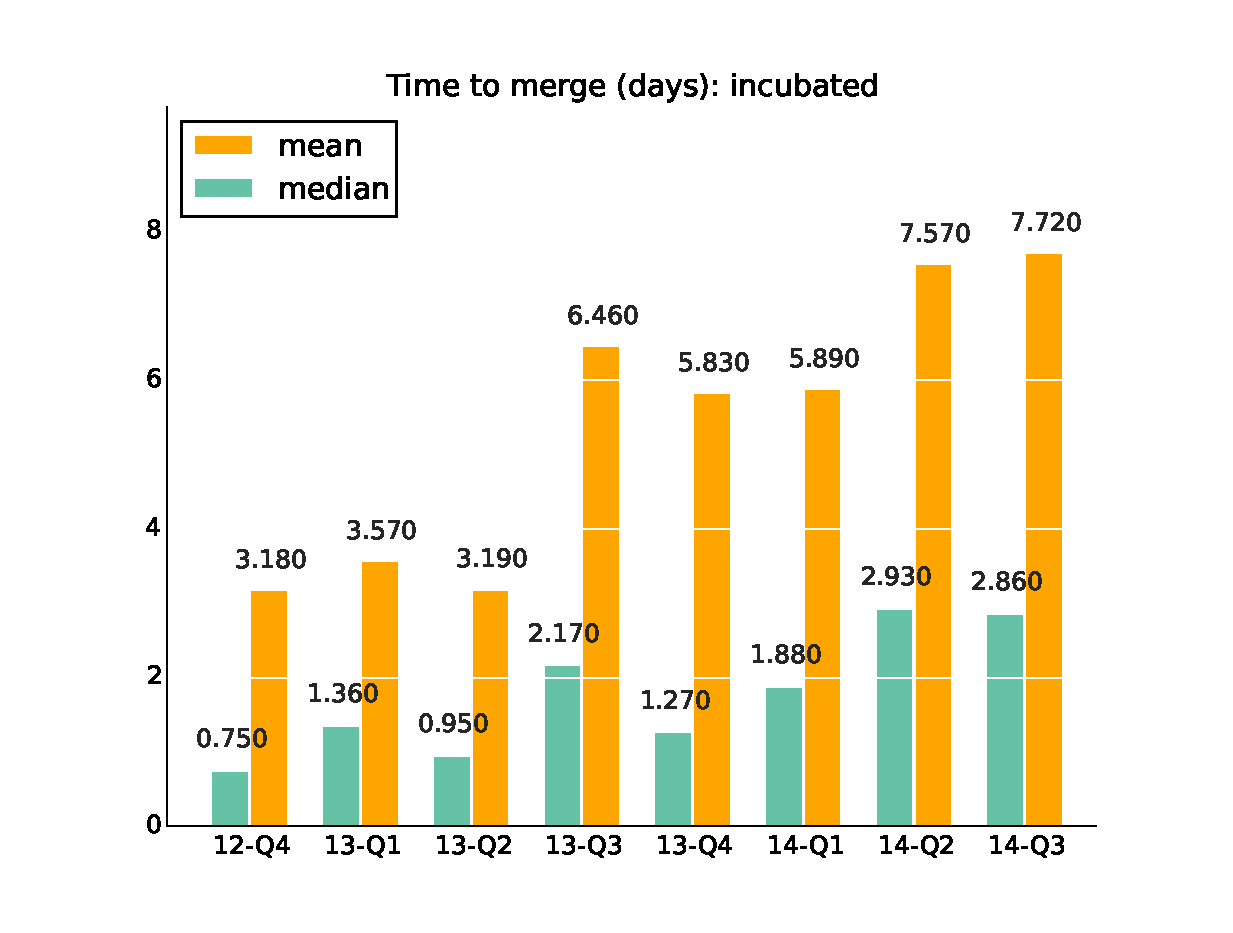
\includegraphics[scale=.35]{figs/timetoreview_medianincubated.eps}
    & 
    \vspace{0pt}
    \begin{tabular}{l|r|r|}%
    \bfseries Period & \bfseries Median & \bfseries Mean % specify table head
    \csvreader[head to column names]{data/timetoreview_medianincubated.csv}{}% use head of csv as column names
    {\\\labels & \mediantime & \meantime}
    \end{tabular}
\end{tabular}

\begin{tabular}{p{7cm} p{5cm}}
    \vspace{0pt} 
    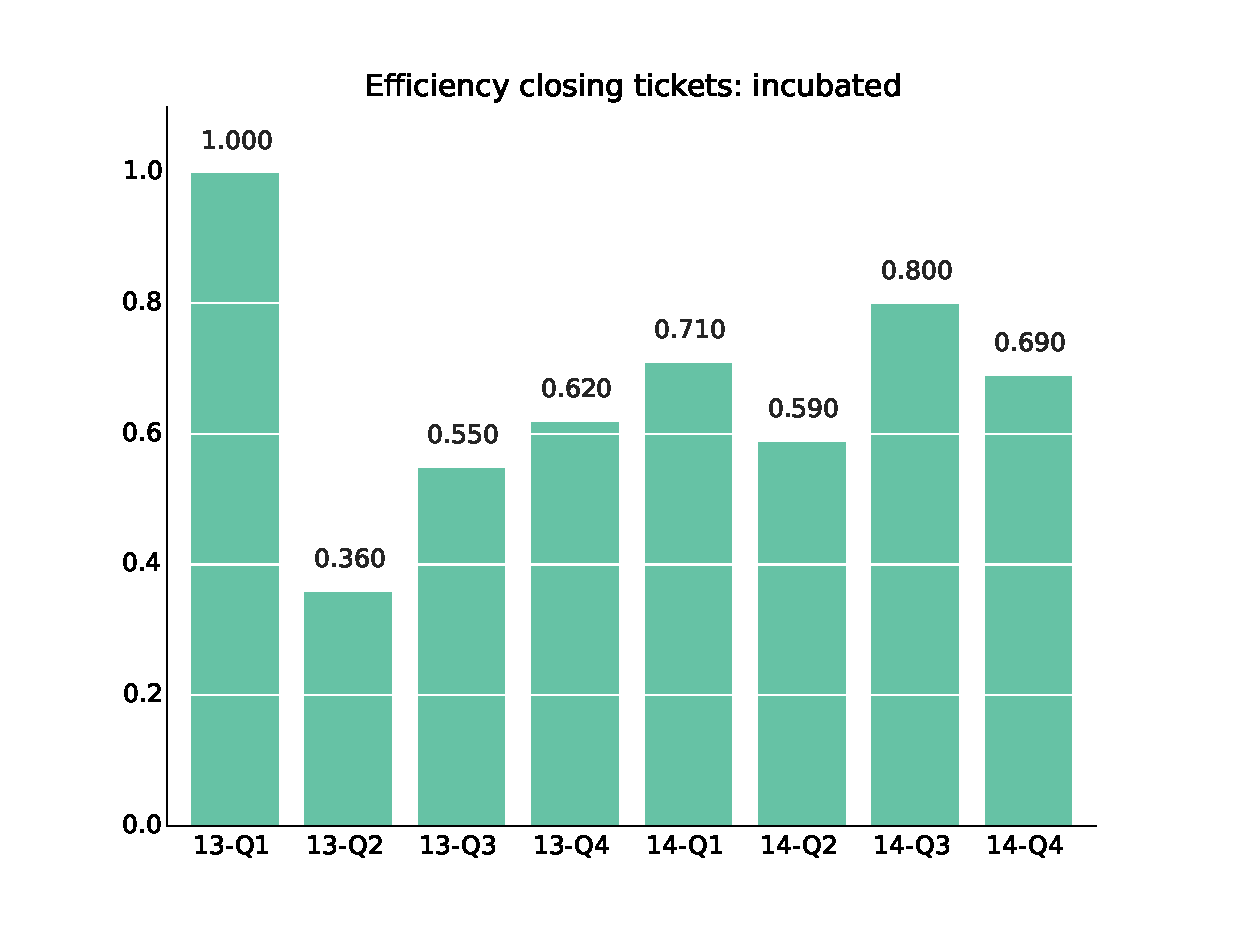
\includegraphics[scale=.35]{figs/bmiincubated.eps}
    & 
    \vspace{0pt}
    \begin{tabular}{l|l}%
    \bfseries Period & \bfseries Closed/Opened % specify table head
    \csvreader[head to column names]{data/bmiincubated.csv}{}% use head of csv as column names
    {\\\labels & \bmi}
    \end{tabular}
\end{tabular}

\begin{tabular}{p{7cm} p{5cm}}
    \vspace{0pt} 
    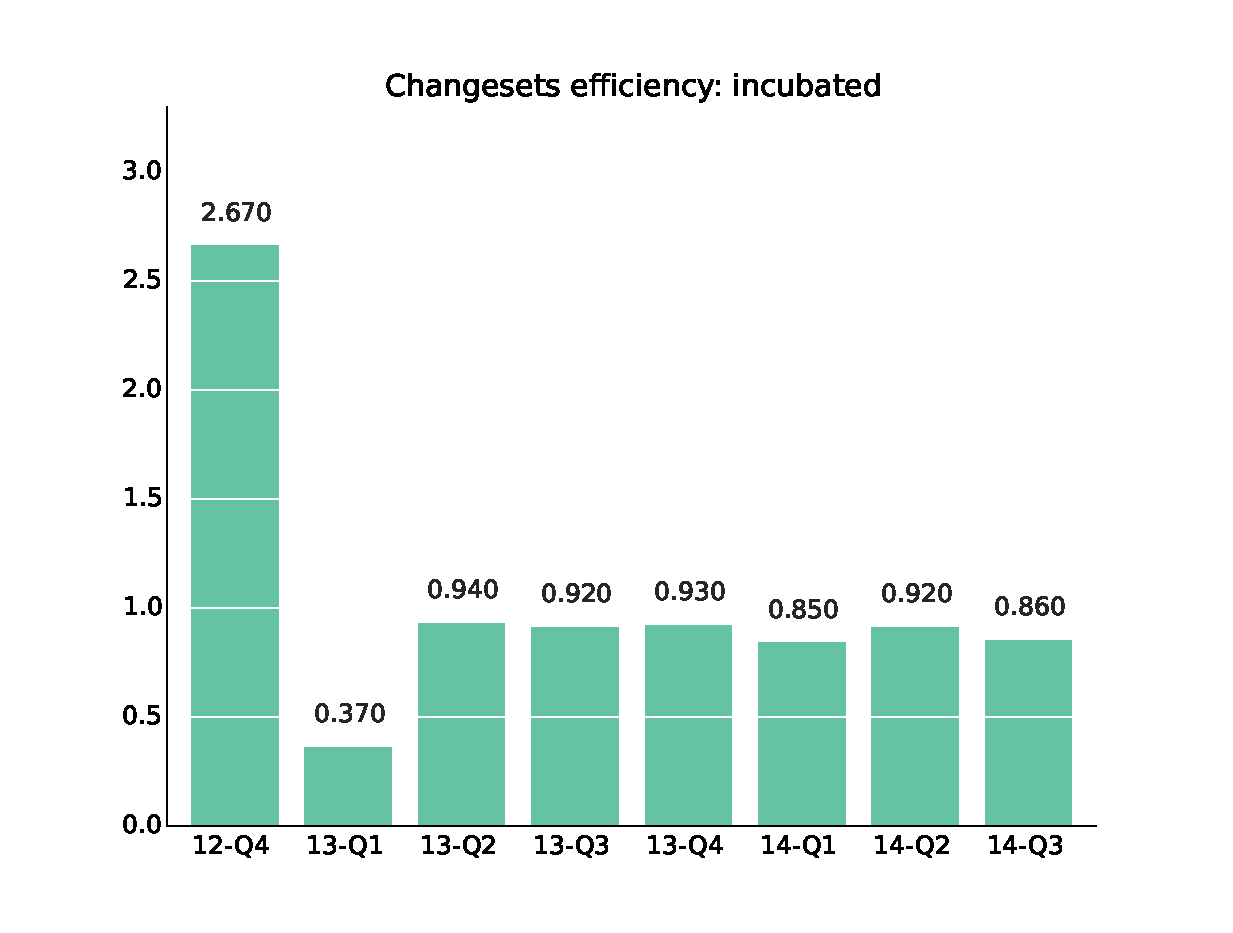
\includegraphics[scale=.35]{figs/bmiscrincubated.eps}
    & 
    \vspace{0pt}
    \begin{tabular}{l|l}%
    \bfseries Period & \bfseries (Aband. and Merg.)/Subm. % specify table head
    \csvreader[head to column names]{data/submitted_reviewsincubated.csv}{}% use head of csv as column names
    {\\\labels & \bmi}
    \end{tabular}
\end{tabular}



\begin{tabular}{p{7cm} p{5cm}}
    \vspace{0pt} 
    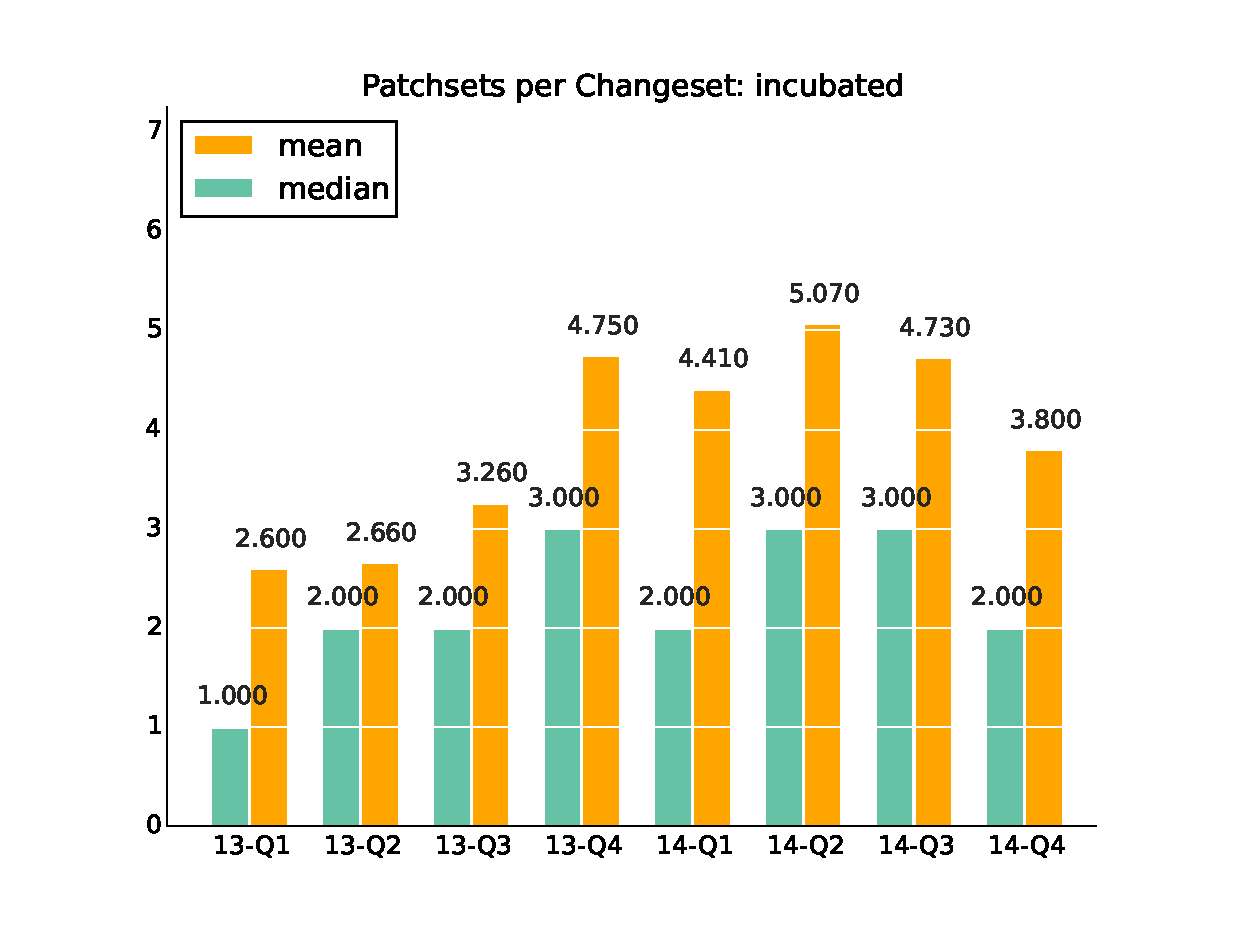
\includegraphics[scale=.35]{figs/patchsets_avgincubated.eps}
    & 
    \vspace{0pt}
    \begin{tabular}{l|r|r|}%
    \bfseries Period & \bfseries Median & \bfseries Mean % specify table head
    \csvreader[head to column names]{data/scr_patchsets_iterationsincubated.csv}{}% use head of csv as column names
    {\\\labels & \medianpatchsets & \meanpatchsets}
    \end{tabular}
\end{tabular}

\begin{tabular}{p{7cm} p{5cm}}
    \vspace{0pt} 
    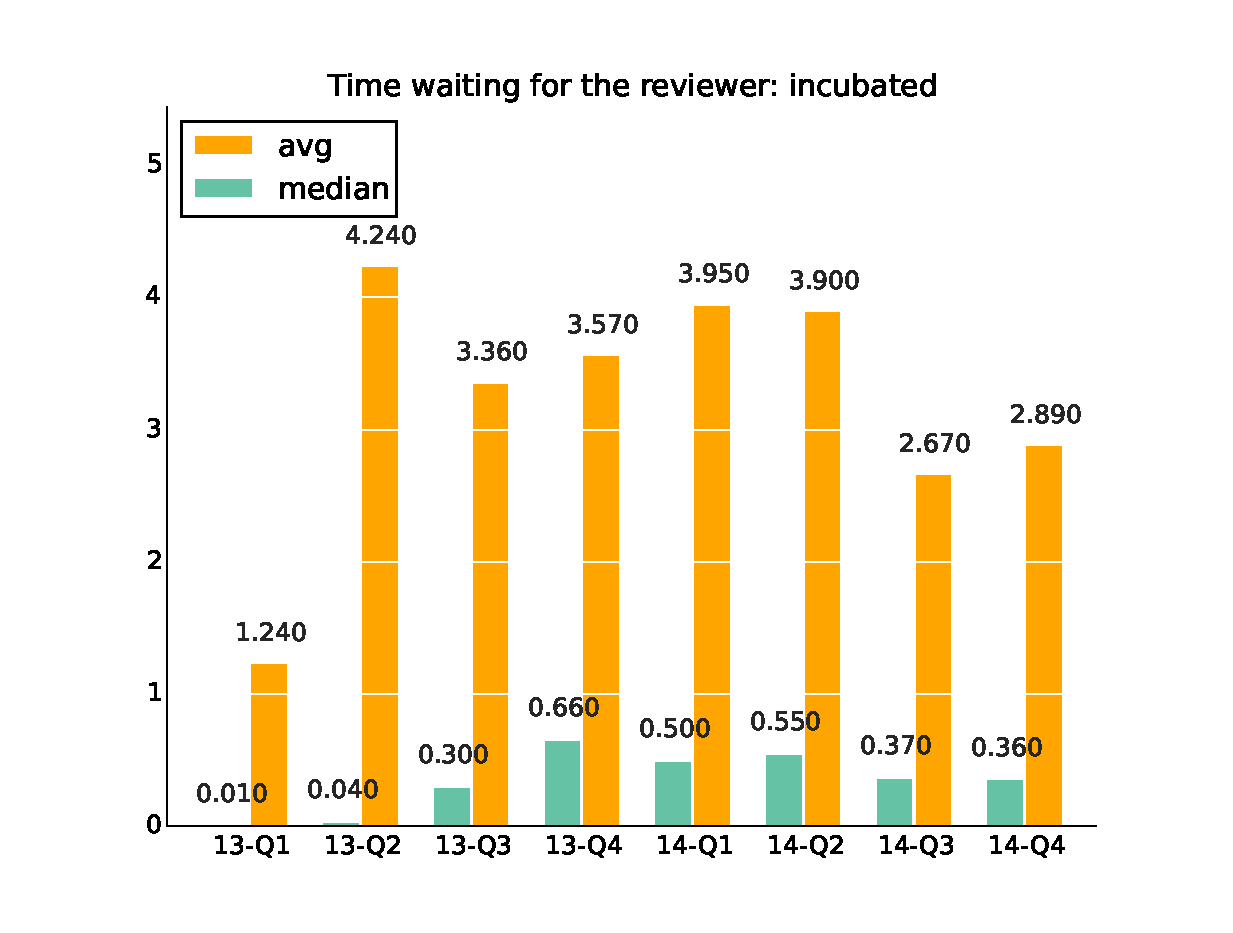
\includegraphics[scale=.35]{figs/waiting4reviewer_avgincubated.eps}
    & 
    \vspace{0pt}
    \begin{tabular}{l|r|r|}%
    \bfseries Period & \bfseries Median & \bfseries Mean % specify table head
    \csvreader[head to column names]{data/timewaiting4reviewer_medianincubated.csv}{}% use head of csv as column names
    {\\\labels & \mediantime & \meantime}
    \end{tabular}
\end{tabular}

\begin{tabular}{p{7cm} p{5cm}}
    \vspace{0pt} 
    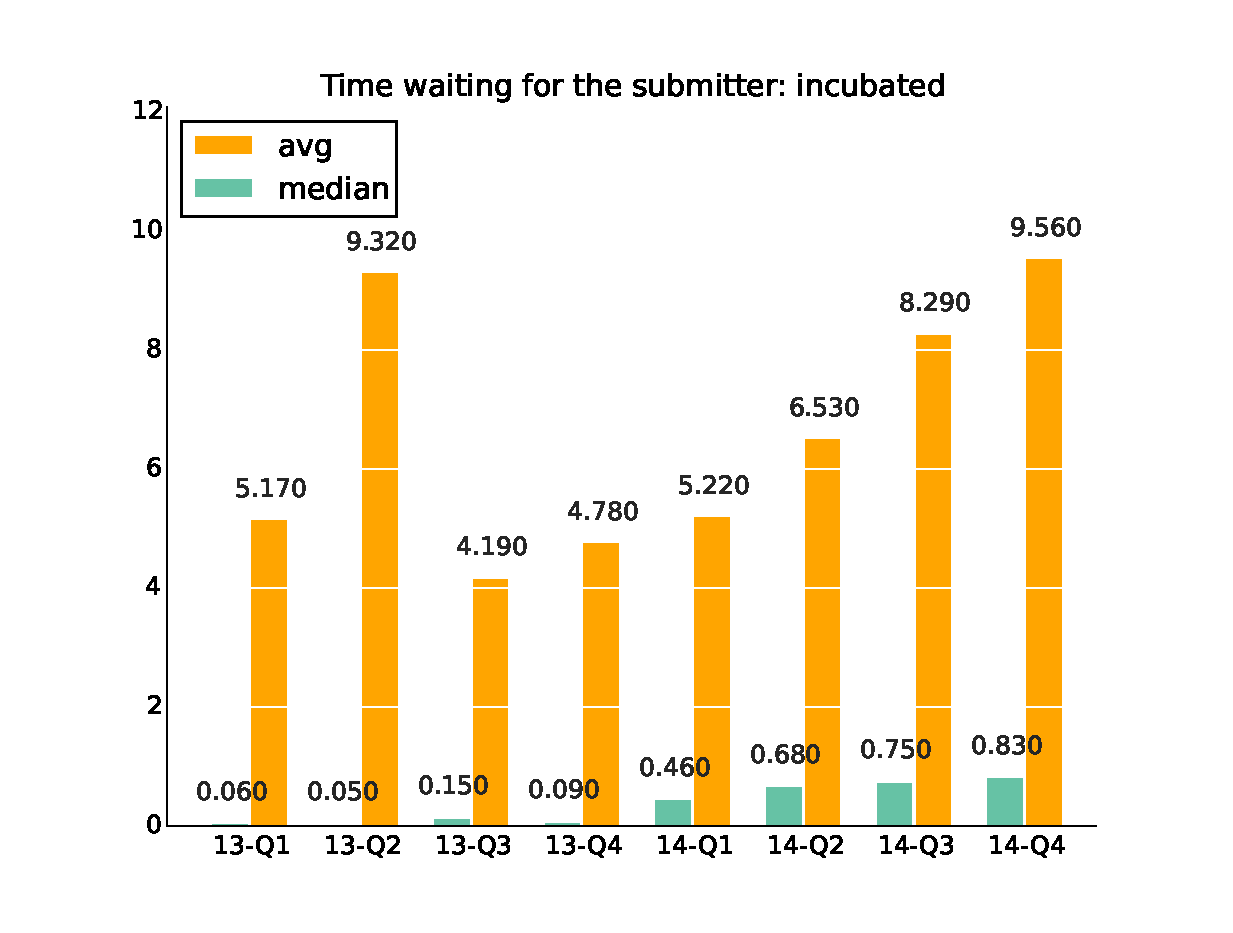
\includegraphics[scale=.35]{figs/waiting4submitter_avgincubated.eps}
    & 
    \vspace{0pt}
    \begin{tabular}{l|r|r|}%
    \bfseries Period & \bfseries Median & \bfseries Mean % specify table head
    \csvreader[head to column names]{data/timewaiting4submitter_medianincubated.csv}{}% use head of csv as column names
    {\\\labels & \mediantime & \meantime}
    \end{tabular}
\end{tabular}



\chapter{General Activity and Community Evolution}

\section{Git Community Structure}

\begin{tabular}{p{7cm} p{5cm}}
    \vspace{0pt} 
    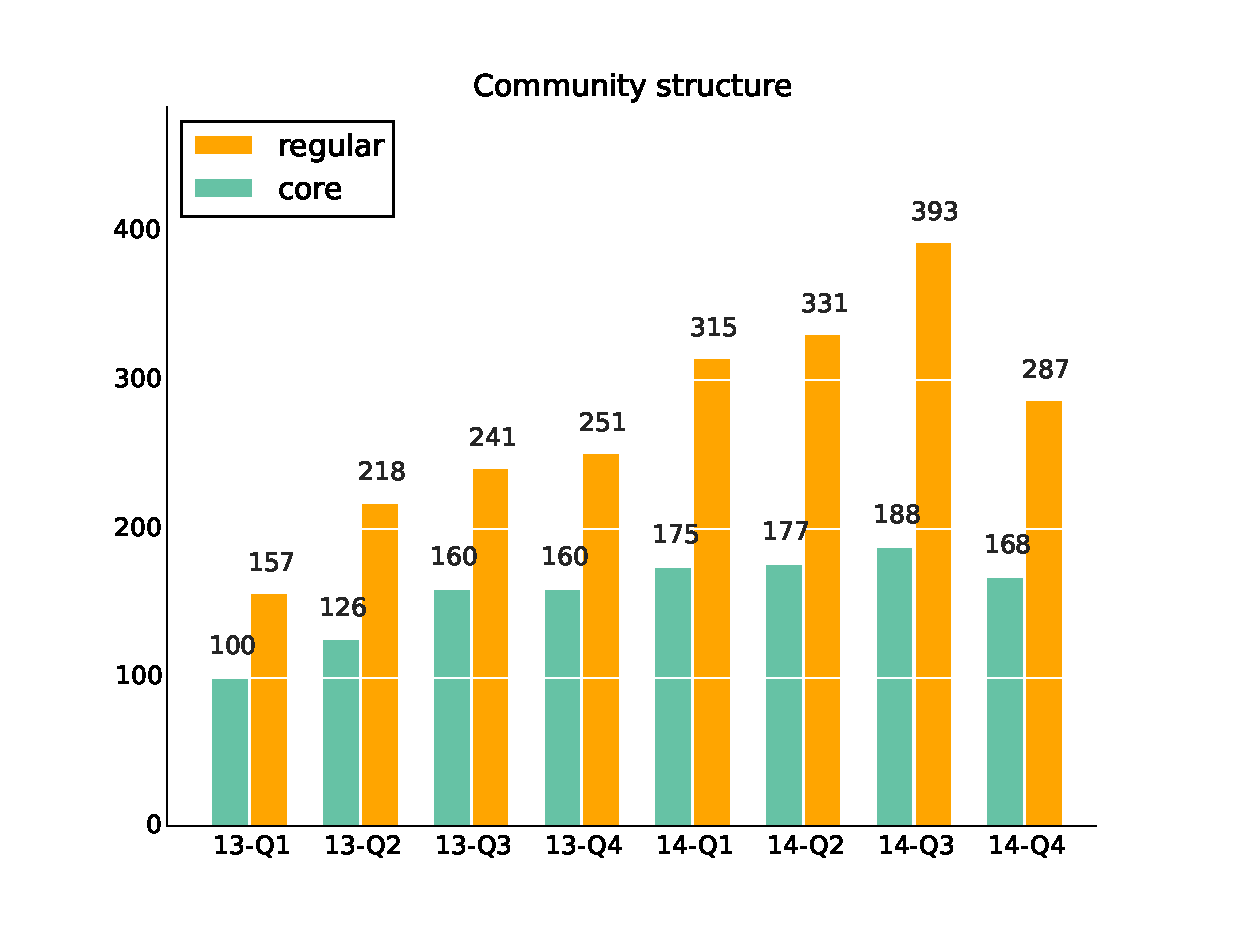
\includegraphics[scale=.35]{figs/onion.eps}
    & 
    \vspace{0pt}
    \begin{tabular}{l|r|r|r|}%
    \bfseries Period & \bfseries Core & \bfseries Regular & \bfseries Occasional% specify table head
    \csvreader[head to column names]{data/onion_model.csv}{}% use head of csv as column names
    {\\\labels & \core & \regular & \occasional}
    \end{tabular}
\end{tabular}


\textbf{Developers per Month}

\begin{tabular}{p{7cm} p{5cm}}
    \vspace{0pt} 
    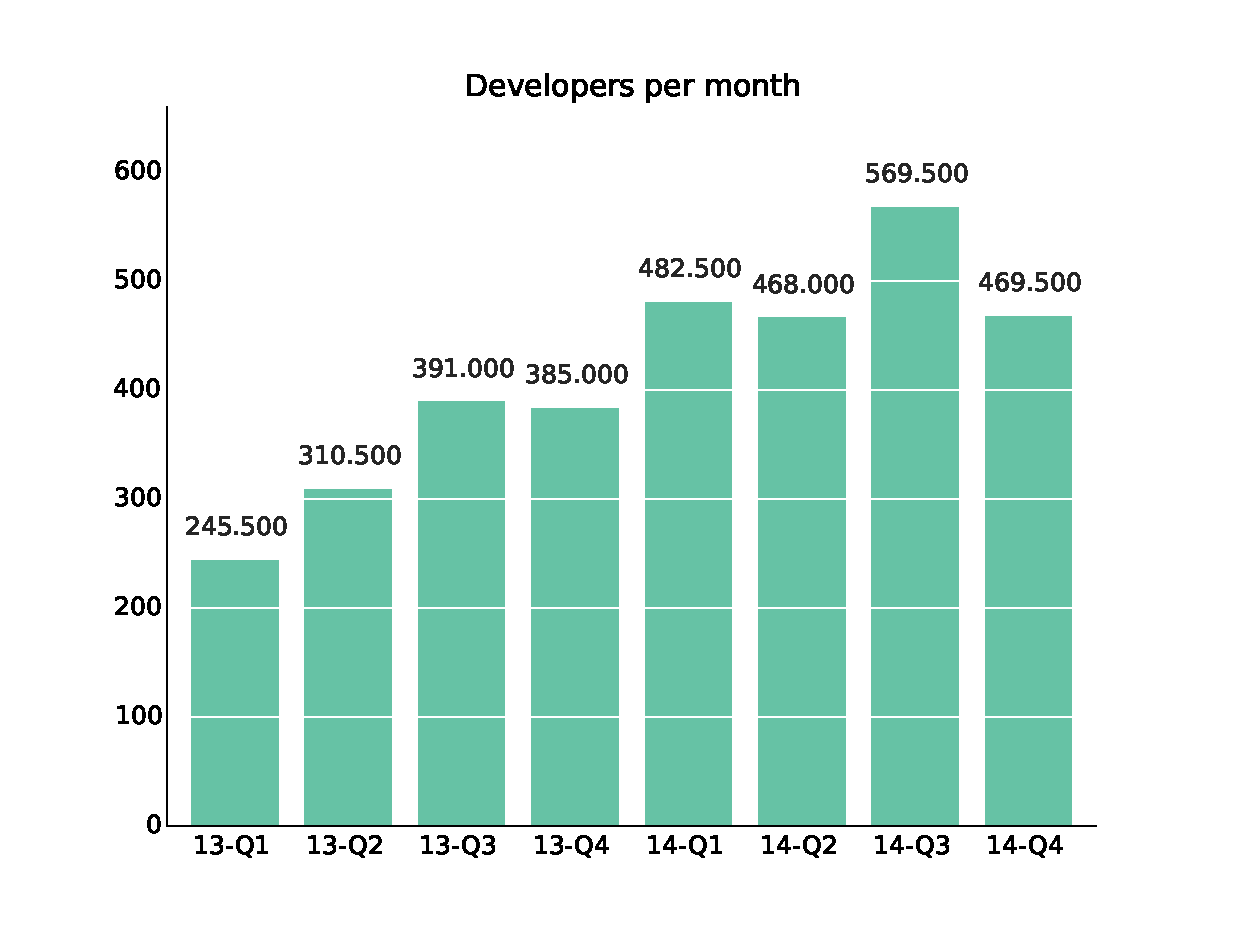
\includegraphics[scale=.35]{figs/authors_month.eps}
    & 
    \vspace{0pt}
    \begin{tabular}{l|r|}%
    \bfseries Period & \bfseries Authors per month% specify table head
   \csvreader[head to column names]{data/authors_month.csv}{}% use head of csv as column names
   {\\\labels & \authormonth}
   \end{tabular}
\end{tabular}

\section{Mailing Lists}

\begin{tabular}{p{7cm} p{5cm}}
    \vspace{0pt} 
    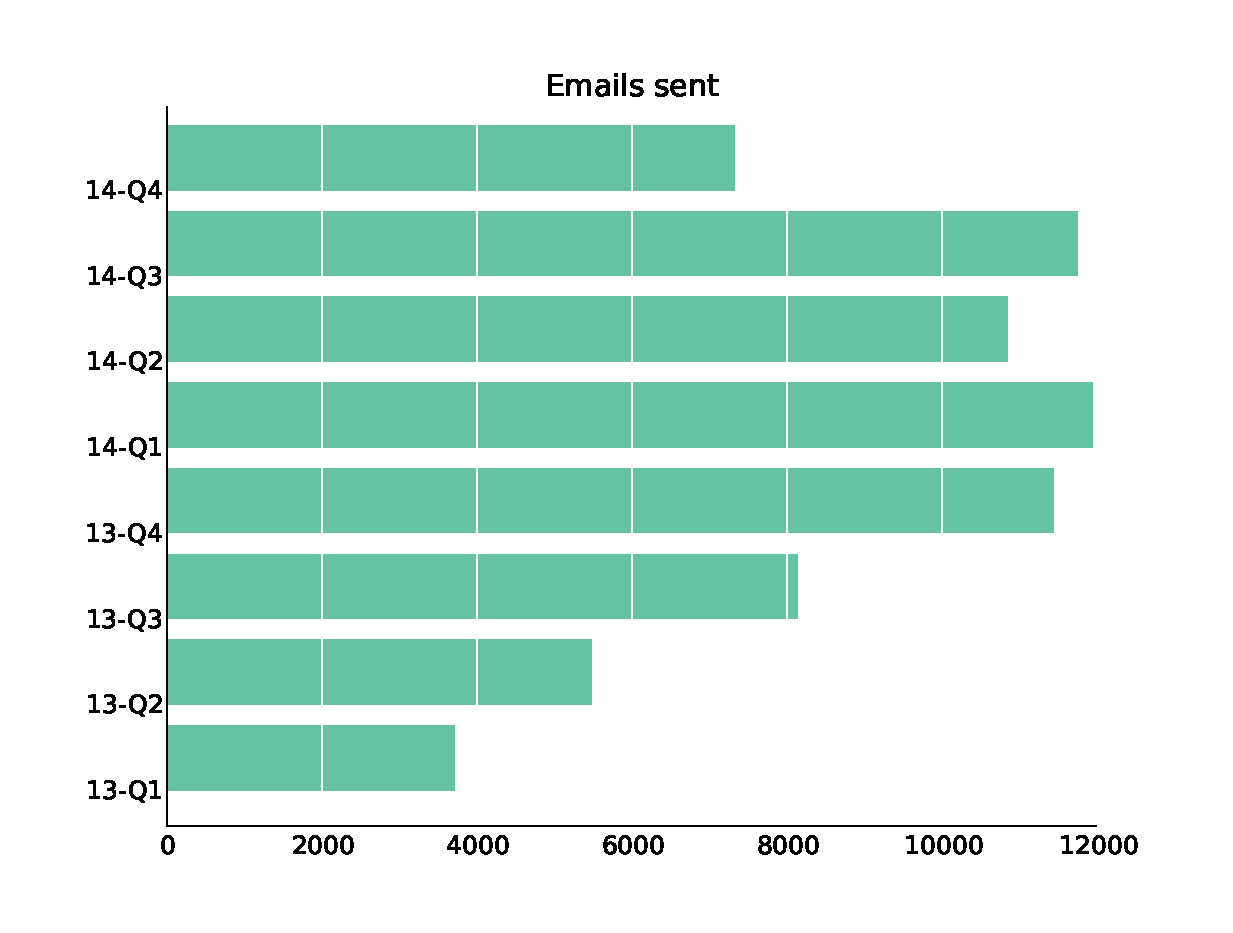
\includegraphics[scale=.35]{figs/emails.eps}
    & 
    \vspace{0pt}
    \begin{tabular}{l|l}%
    \bfseries Period & \bfseries Emails % specify table head
    \csvreader[head to column names]{data/emails.csv}{}% use head of csv as column names
    {\\\labels & \emails}
    \end{tabular}
\end{tabular}

\begin{tabular}{p{7cm} p{5cm}}
    \vspace{0pt} 
    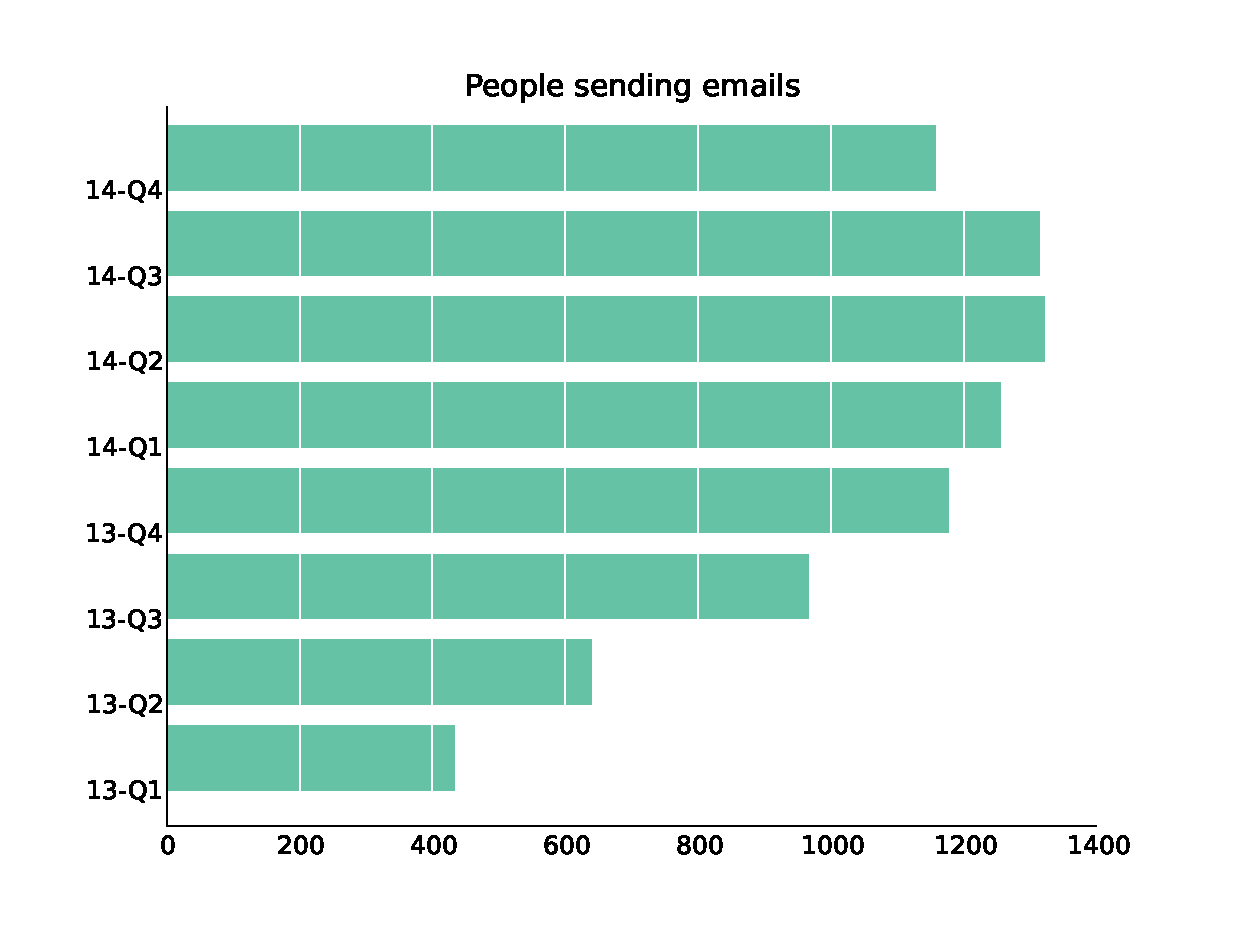
\includegraphics[scale=.35]{figs/emails_senders.eps}
    & 
    \vspace{0pt}
    \begin{tabular}{l|l}%
    \bfseries Period & \bfseries People % specify table head
    \csvreader[head to column names]{data/emails_senders.csv}{}% use head of csv as column names
    {\\\labels & \senders}
    \end{tabular}
\end{tabular}

\begin{tabular}{p{7cm} p{5cm}}
    \vspace{0pt} 
    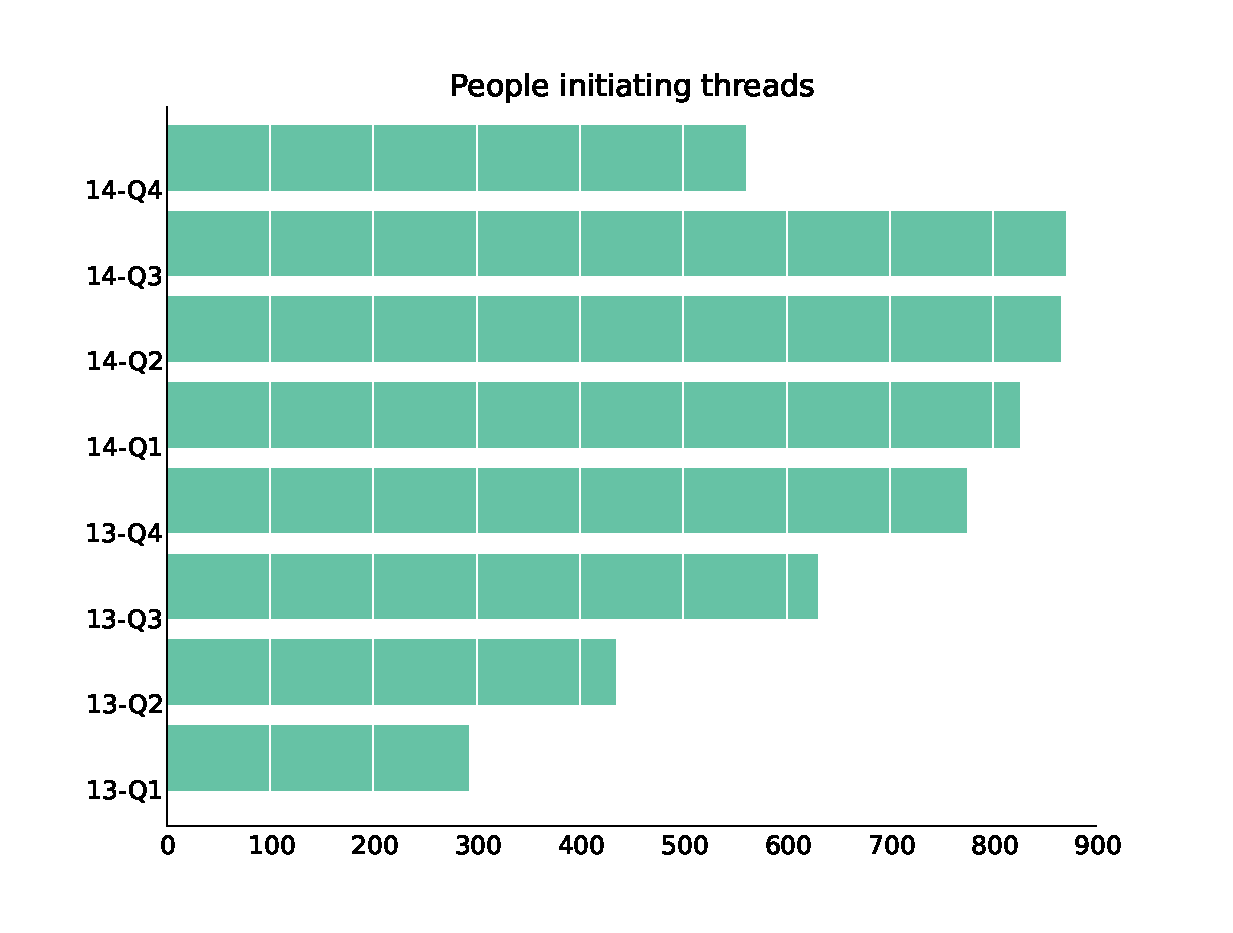
\includegraphics[scale=.35]{figs/emails_senders_init.eps}
    & 
    \vspace{0pt}
    \begin{tabular}{l|l}%
    \bfseries Period & \bfseries People % specify table head
    \csvreader[head to column names]{data/emails_senders_init.csv}{}% use head of csv as column names
    {\\\labels & \senders}
    \end{tabular}
\end{tabular}

\begin{tabular}{p{4cm}p{5cm}p{2cm}}
    \bfseries Initial Author &  & \bfseries Number \\ 
    \bfseries and Date       & \bfseries Subject  & \bfseries Messages% specify table head
    \csvreader[head to column names]{data/mls_top_longest_threads.csv}{}% use head of csv as column names
    {\\\initiator \\\date & \subject & \len}
   % {\\\hline\csvcoli & \csvcolvii & \csvcolv & \csvcolii}% specify your coloumns here
\end{tabular}


\begin{tabular}{p{3cm}p{6cm}p{2cm}}
    \bfseries Initial Author & & \bfseries Diff. \\
    \bfseries and Date & \bfseries Subject  &  \bfseries People% specify table head
    \csvreader[head to column names]{data/mls_top_crowded_threads.csv}{}% use head of csv as column names
    {\\\initiator \\\date & \subject  & \people}
   % {\\\hline\csvcoli & \csvcolvii & \csvcolv & \csvcolii}% specify your coloumns here
\end{tabular}

%\begin{tabular}{p{5cm}p{3cm}p{2cm}}
%    \bfseries Initial Author & \bfseries Subject  & \bfseries Date % specify table head
%    \csvreader[head to column names]{data/mls_top_longest_threads.csv}{}% use head of csv as column names
%    {\\\hline\csvcoli & \csvcolvi & \csvcoliv }% specify your coloumns here
%\end{tabular}

\section{Questions and Answers}

\begin{tabular}{p{7cm} p{5cm}}
    \vspace{0pt} 
    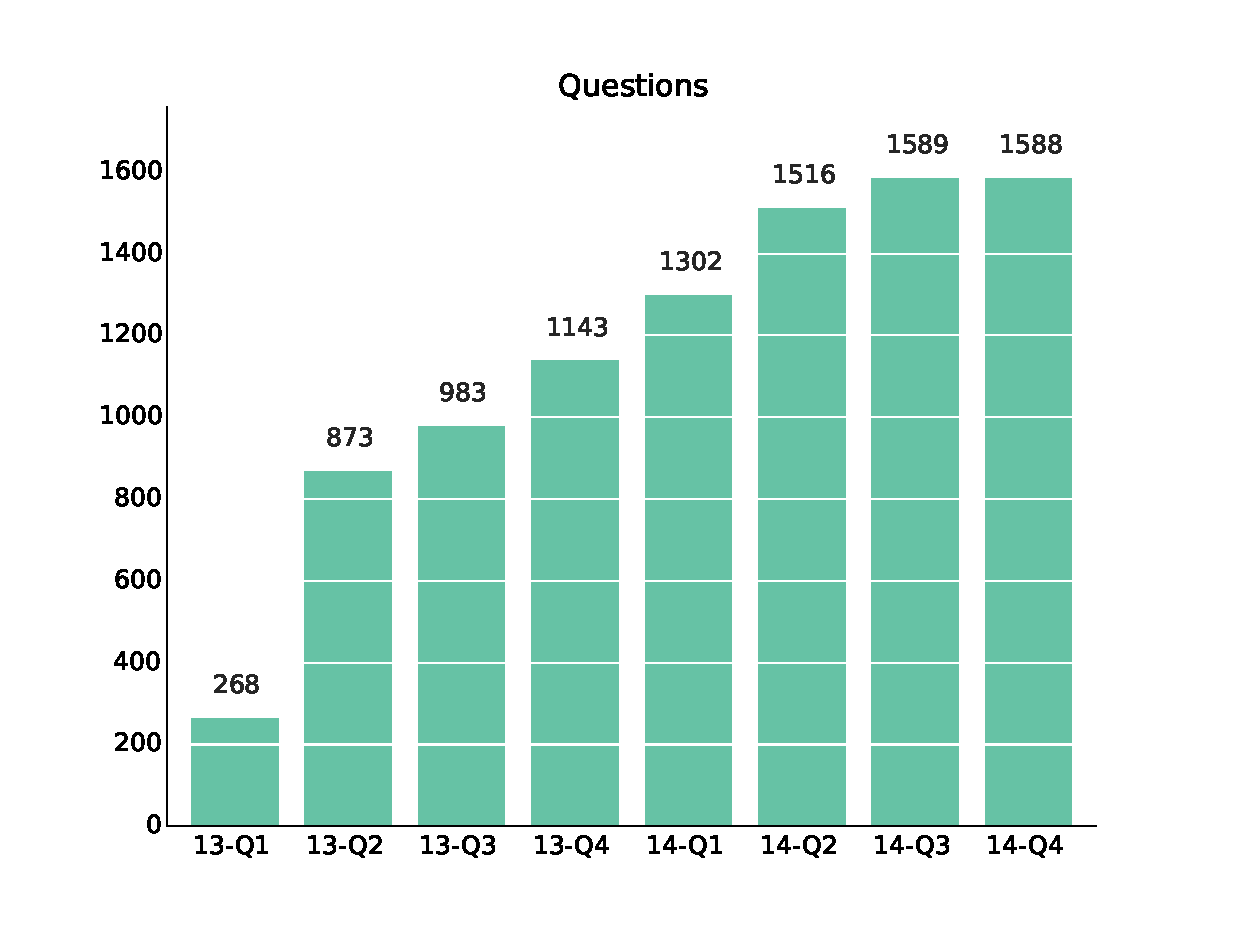
\includegraphics[scale=.35]{figs/questions.eps}
    & 
    \vspace{0pt}
    \begin{tabular}{l|l}%
    \bfseries Period & \bfseries Questions % specify table head
    \csvreader[head to column names]{data/questions.csv}{}% use head of csv as column names
    {\\\labels & \questions}
    \end{tabular}
\end{tabular}

\begin{tabular}{p{7cm} p{5cm}}
    \vspace{0pt} 
    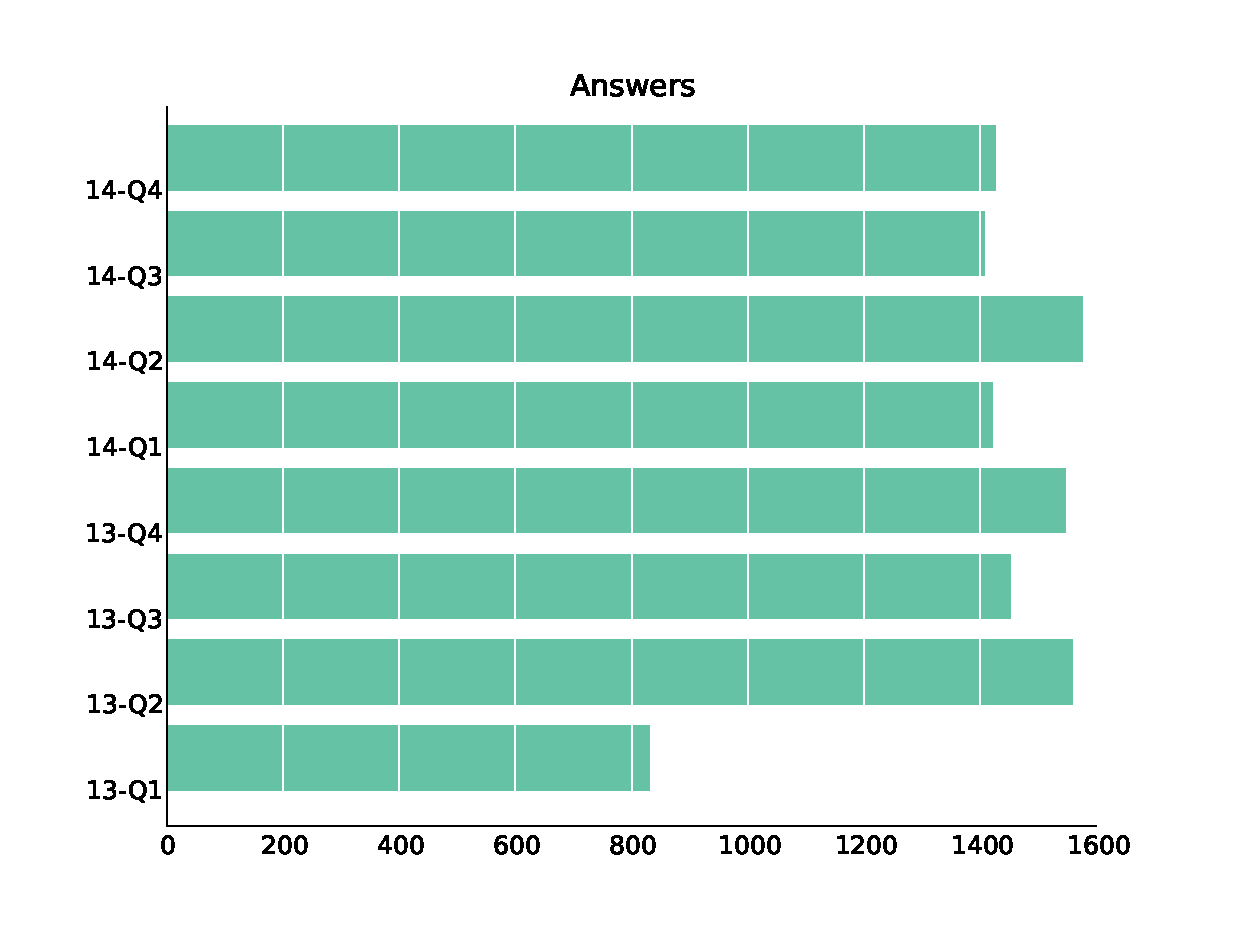
\includegraphics[scale=.35]{figs/answers.eps}
    & 
    \vspace{0pt}
    \begin{tabular}{l|l}%
    \bfseries Period & \bfseries Answers % specify table head
    \csvreader[head to column names]{data/answers.csv}{}% use head of csv as column names
    {\\\labels & \answers}
    \end{tabular}
\end{tabular}

\begin{tabular}{p{7cm} p{5cm}}
    \vspace{0pt} 
    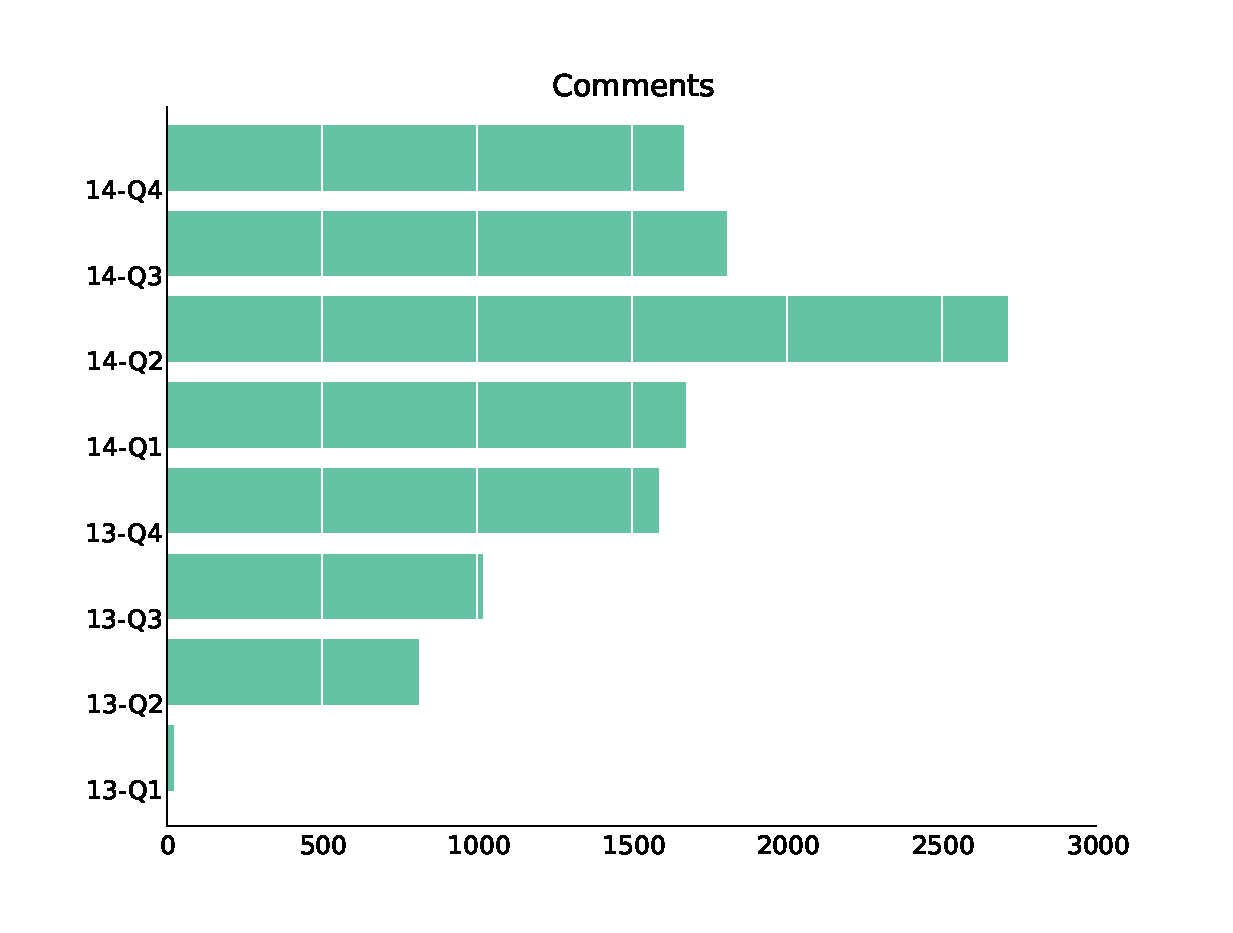
\includegraphics[scale=.35]{figs/comments.eps}
    & 
    \vspace{0pt}
    \begin{tabular}{l|l}%
    \bfseries Period & \bfseries Comments % specify table head
    \csvreader[head to column names]{data/comments.csv}{}% use head of csv as column names
    {\\\labels & \comments}
    \end{tabular}
\end{tabular}

\begin{tabular}{p{7cm} p{5cm}}
    \vspace{0pt} 
    \includegraphics[scale=.35]{figs/question_senders.eps}
    & 
    \vspace{0pt}
    \begin{tabular}{l|l}%
    \bfseries Period & \bfseries People asking % specify table head
    \csvreader[head to column names]{data/question_senders.csv}{}% use head of csv as column names
    {\\\labels & \senders}
    \end{tabular}
\end{tabular}

\begin{itemize}
\item  Top visited questions.
\end{itemize}

\begin{tabular}{p{8cm}p{2cm}}
    \bfseries Question subject & \bfseries Visits % specify table head
    \csvreader[head to column names]{data/qa_top_questions_visited.csv}{}% use head of csv as column names
    {\\\subject \href{\site}{+} & \visits}
\end{tabular}\\

\begin{itemize}
\item Top questions with more comments.
\end{itemize}
\begin{tabular}{p{8cm}p{2cm}}
    \bfseries Question subject & \bfseries Comments % specify table head
    \csvreader[head to column names]{data/qa_top_questions_commented.csv}{}% use head of csv as column names
    {\\ \subject \href{\site}{+} & \comments}
   % {\\\hline\csvcoli & \csvcolvii & \csvcolv & \csvcolii}% specify your coloumns here
\end{tabular}\\

\begin{itemize}
\item  Top questions with the highest number of different people participating.
\end{itemize}
\begin{tabular}{p{8cm}p{2cm}}
    \bfseries Question subject & \bfseries People participating % specify table head
    \csvreader[head to column names]{data/qa_top_questions_crowded.csv}{}% use head of csv as column names
    {\\\subject \href{\site}{+} & \people}
   % {\\\hline\csvcoli & \csvcolvii & \csvcolv & \csvcolii}% specify your coloumns here
\end{tabular}

\begin{itemize}
\item  Top tags
\end{itemize}
\begin{tabular}{p{8cm}p{2cm}}
    \bfseries Tag name & \bfseries Ocurrences % specify table head
    \csvreader[head to column names]{data/qa_top_tags.csv}{}% use head of csv as column names
    {\\\tag & \occurrences}
   % {\\\hline\csvcoli & \csvcolvii & \csvcolv & \csvcolii}% specify your coloumns here
\end{tabular}

\section{IRC}

\begin{tabular}{p{7cm} p{5cm}}
    \vspace{0pt} 
    \includegraphics[scale=.35]{figs/irc_sent.eps}
    & 
    \vspace{0pt}
    \begin{tabular}{l|l}%
    \bfseries Period & \bfseries Messages % specify table head
    \csvreader[head to column names]{data/irc_sent.csv}{}% use head of csv as column names
    {\\\labels & \messages}
    \end{tabular}
\end{tabular}

\begin{tabular}{p{7cm} p{5cm}}
    \vspace{0pt} 
    \includegraphics[scale=.35]{figs/irc_senders.eps}
    & 
    \vspace{0pt}
    \begin{tabular}{l|l}%
    \bfseries Period & \bfseries People % specify table head
    \csvreader[head to column names]{data/irc_senders.csv}{}% use head of csv as column names
    {\\\labels & \senders}
    \end{tabular}
\end{tabular}

\begin{tabular}{p{8cm}p{2cm}}
    \bfseries IRC id & \bfseries Messages sent % specify table head
    \csvreader[head to column names]{data/irc_top_senders.csv}{}% use head of csv as column names
    {\\\senders & \sent}
   % {\\\hline\csvcoli & \csvcolvii & \csvcolv & \csvcolii}% specify your coloumns here
\end{tabular}

\appendix{}

\chapter{Metrics Definitions}
\label{chap:metrics_definitions}

Metrics depicted in each OpenStack program:

\begin{itemize}
\item Commit: this is defined as the action(s) that performes a change in the source code. 
Bots, merges and other type of automatic activity is removed from the records. Besides,
when aggregating several Gits, this metric only counts unique revisions (unique hashes found in the Git repositories).
Finally, all branches are aggregated to the analysis.

\item Submitted changeset: a changeset is the process of peer reviewing source code changes. A commit
is not merged to the master code of a given project till this is approved for at least one core
reviewer of such project. A submitted changeset is defined as any changeset submitted to the Gerrit
system. However, given the limitations of the current version of the tool, with at least 5,900 changesets
detected as having an erroneous creation date, this metric counts the first patchset upload action. 
 
\item Merged and abandoned changsets: a merge is defined as the patchset that was finally submitted to the 
source code. An abandoned changeset is a potential merge that was finally dismissed by developers as
being part of the source code. This status is found in the status of the final patchset. However, although
a patchset can be merged or abandoned, this action can be reverted. If a patchset presents several of 
these changes in the same period of time, only one of them is counted (the very last one). On the other hand,
if those changes take place in different periods of analysis, both status would be counted.

\item Open and closed ticket: a ticket in Launchpad is counted as closed if the status of such ticket is defined as 'Fix Released'.
The rest of the tickets are counted as opened tickets.

\item Active Core Reviewer: a core reviewer has the possibility to use +2 or -2 actions when reviewing the code. 
However, if there are developers that for some period do not use those actions, those can not be measured as core reviewer.
Thus, this metric provides information about 'active' core reviewers. This can be also defined as those developers
that actively have used the +2 or -2 review action. Besides, this metric is filtered by branch of activity, only using 'master'.
This helps to detect actual core reviewers in each of the projects.

\item Authors: a developer is defined as author if she is the owner of the patchset sent for reviewing and this is 
merged into the source code. As previously indicated, automatic commits such bot's are removed from this analysis.

\item Efficiency closing issues: this metric is a derivation of the Backlog Management Index (BMI) that measures the number
of closed tickets out of the opened tickets in a period of time. Values under 1.0 indicates that the number of closing
issues is lower than the number of opened issues arriving. On the contrary, higher charts would indicate better
maintenance effort by the community.

\item Efficiency closing changesets: this metric is a derivation of the Backlog Management Index as it is named as
Review efficiency index (REI). As similarly used in the BMI index, this metrics measures the number of closed changesets
(merged or abandoned) out of the total number of new changesets.

\item Time to Merge: this time consists of the time between the first upload of the first patchset (as defined
as a submitted changeset) till the last patchset of the changeset is merged into the code and this is indicated in the 
comments side of the Gerrit tool. This metric is provided in number of days.

\item Patchsets per changeset: this metric calculates the total number of iterations in a changeset till this is abandoned
or merged.

\item Time waiting for the reviewer or the submitter: a changeset is waiting for a reviewer action if a new patchset upload
or a new changset arrives to the system. On the other hand, a submitter action is required when a specific negative verification
or reviewing action takes place (Verified -1/-2 or Code-Review -1/-2). In addition, when a Code-Review +2 action takes place,
it is assumed that the changset is closing and no more times are registered either for the reviewer or the submitter.
For this analysis, those patchsets flagged as work in progress are ignored.

\end{itemize}

Metrics depicted in the general overview:

\begin{itemize}
\item Community structure, core, regular and casual developers: developers are ordered in descendant order by the
number of commits authored for a given period. Core developers are defined as the list of developers that 
reach 80\% of the total commits. Regular is the set of developers that are between that 80\% and 95\% of the commits.
Casual developers are found in the rest of the 5\%. Bots are ignored in this list of developers.

\item Developer per month: average of developers per month ignoring bots.

\item Emails sent: number of emails sent by people to the several mailing lists. Bots are not registered.

\item People sending emails: number of people sending those emails ignoring bots.

\item People initiating threads: a thread is defined as a list of emails that has the same root. There may exist
threads of one email.

\item Top threads: this list provides the longest threads in terms of number of emails that have a common root email.

\item Questions, answers and comments in Askbot.

\item People asking questions in Askbot: number of people sending a new question.

\item Top visited questions.

\item Top tags: each of the questions has a list of associated tags. The top tags  are those 
with the highest number of repetitions aggregating all of the questions.

\item Messages and people in IRC: this analysis ignores as a message those entries in the IRC channels that provide
information about people entering or leaving the system.  

\end{itemize}



\chapter{Source Code and Data Sources}
\label{chap:data_sources}

The data source used to provide the data of this analysis can be found at the GrimoireLib library. Specifically the openstack\_report.py file\footnote{\url{https://github.com/VizGrimoire/GrimoireLib/blob/master/vizGrimoireJS/openstack_report.py}. In order to download the exact version used for this analysis with the hash \emph{xxxx}}. 


With respect to the list of analyzed repositories per project, the following table lists all of them.
There are three data sources: git activity (scm), tickets activity (its) and review activity (scr). This information is based on the information listed in the yaml organizational file\footnote{url{http://git.openstack.org/cgit/openstack/governance/tree/reference/programs.yaml}} provided by the OpenStack Foundation.

%select p.id, pr.data_source, pr.repository_name 
%from projects p, project_repositories pr 
%where p.project_id=pr.project_id order by p.id, pr.data_source;

\begin{center}                                                                       
\begin{longtable}{|p{4cm}|p{1cm}|p{10cm}|}
\hline
Program & Data source & Repository \\
\hline


app-catalog&scm&git://git.openstack.org/openstack/app-catalog\\ 
app-catalog&scm&git://git.openstack.org/openstack/app-catalog-ui\\ 
app-catalog&scm&git://git.openstack.org/openstack/app-catalog-common\\ 
app-catalog&scr&review.openstack.org\_openstack/app-catalog\\ 
app-catalog&scr&review.openstack.org\_openstack/app-catalog-common\\ 
app-catalog&scr&review.openstack.org\_openstack/app-catalog-ui\\ 
Astara&scm&git://git.openstack.org/openstack/astara-appliance\\ 
Astara&scm&git://git.openstack.org/openstack/astara-horizon\\ 
Astara&scm&git://git.openstack.org/openstack/astara\\ 
Astara&scm&git://git.openstack.org/openstack/astara-neutron\\ 
Astara&scr&review.openstack.org\_openstack/astara-horizon\\ 
Astara&scr&review.openstack.org\_openstack/astara\\ 
Astara&scr&review.openstack.org\_openstack/astara-neutron\\ 
Astara&scr&review.openstack.org\_openstack/astara-appliance\\ 
barbican&its&https://bugs.launchpad.net/barbican\\ 
barbican&scm&git://git.openstack.org/openstack/kite\\ 
barbican&scm&git://git.openstack.org/openstack/python-kiteclient\\ 
barbican&scm&git://git.openstack.org/openstack/python-barbicanclient\\ 
barbican&scm&git://git.openstack.org/openstack/barbican\\ 
barbican&scm&git://git.openstack.org/openstack/castellan\\ 
barbican&scr&review.openstack.org\_openstack/python-barbicanclient\\ 
barbican&scr&review.openstack.org\_openstack/castellan\\ 
barbican&scr&review.openstack.org\_openstack/kite\\ 
barbican&scr&review.openstack.org\_openstack/barbican\\ 
barbican&scr&review.openstack.org\_openstack/python-kiteclient\\ 
ceilometer&its&https://bugs.launchpad.net/python-ceilometerclient\\ 
ceilometer&its&https://bugs.launchpad.net/ceilometer\\ 
ceilometer&scm&https://github.com/openstack/ceilometer.git\\ 
ceilometer&scm&git://git.openstack.org/openstack/gnocchi\\ 
ceilometer&scm&git://git.openstack.org/openstack/aodh\\ 
ceilometer&scm&https://github.com/openstack/python-ceilometerclient.git\\ 
ceilometer&scm&git://git.openstack.org/openstack/ceilometermiddleware\\ 
ceilometer&scm&git://git.openstack.org/openstack/python-gnocchiclient\\ 
ceilometer&scr&review.openstack.org\_openstack/aodh\\ 
ceilometer&scr&review.openstack.org\_openstack/python-ceilometerclient\\ 
ceilometer&scr&review.openstack.org\_openstack/python-gnocchiclient\\ 
ceilometer&scr&review.openstack.org\_openstack/ceilometer\\ 
ceilometer&scr&review.openstack.org\_openstack/ceilometermiddleware\\ 
ChefOpenStack&its&https://bugs.launchpad.net/openstack-chef\\ 
ChefOpenStack&scm&git://git.openstack.org/openstack/cookbook-openstack-block-storage\\ 
ChefOpenStack&scm&git://git.openstack.org/openstack/cookbook-openstack-data-processing\\ 
ChefOpenStack&scm&git://git.openstack.org/openstack/cookbook-openstack-network\\ 
ChefOpenStack&scm&git://git.openstack.org/openstack/cookbook-openstack-telemetry\\ 
ChefOpenStack&scm&git://git.openstack.org/openstack/cookbook-openstack-compute\\ 
ChefOpenStack&scm&git://git.openstack.org/openstack/cookbook-openstack-image\\ 
ChefOpenStack&scm&git://git.openstack.org/openstack/cookbook-openstack-ops-database\\ 
ChefOpenStack&scm&git://git.openstack.org/openstack/cookbook-openstack-client\\ 
ChefOpenStack&scm&git://git.openstack.org/openstack/cookbook-openstack-database\\ 
ChefOpenStack&scm&git://git.openstack.org/openstack/cookbook-openstack-object-storage\\ 
ChefOpenStack&scm&git://git.openstack.org/openstack/openstack-chef-repo\\ 
ChefOpenStack&scm&git://git.openstack.org/openstack/cookbook-openstack-bare-metal\\ 
ChefOpenStack&scm&git://git.openstack.org/openstack/cookbook-openstack-dashboard\\ 
ChefOpenStack&scm&git://git.openstack.org/openstack/cookbook-openstack-integration-test\\ 
ChefOpenStack&scm&git://git.openstack.org/openstack/cookbook-openstack-orchestration\\ 
ChefOpenStack&scm&git://git.openstack.org/openstack/cookbook-openstack-common\\ 
ChefOpenStack&scm&git://git.openstack.org/openstack/cookbook-openstack-identity\\ 
ChefOpenStack&scm&git://git.openstack.org/openstack/cookbook-openstack-ops-messaging\\ 
ChefOpenStack&scr&review.openstack.org\_openstack/cookbook-openstack-client\\ 
ChefOpenStack&scr&review.openstack.org\_openstack/cookbook-openstack-database\\ 
ChefOpenStack&scr&review.openstack.org\_openstack/cookbook-openstack-object-storage\\ 
ChefOpenStack&scr&review.openstack.org\_openstack/openstack-chef-repo\\ 
ChefOpenStack&scr&review.openstack.org\_openstack/cookbook-openstack-dashboard\\ 
ChefOpenStack&scr&review.openstack.org\_openstack/cookbook-openstack-integration-test\\ 
ChefOpenStack&scr&review.openstack.org\_openstack/cookbook-openstack-orchestration\\ 
ChefOpenStack&scr&review.openstack.org\_openstack/cookbook-openstack-common\\ 
ChefOpenStack&scr&review.openstack.org\_openstack/cookbook-openstack-identity\\ 
ChefOpenStack&scr&review.openstack.org\_openstack/cookbook-openstack-ops-messaging\\ 
ChefOpenStack&scr&review.openstack.org\_openstack/cookbook-openstack-bare-metal\\ 
ChefOpenStack&scr&review.openstack.org\_openstack/cookbook-openstack-data-processing\\ 
ChefOpenStack&scr&review.openstack.org\_openstack/cookbook-openstack-network\\ 
ChefOpenStack&scr&review.openstack.org\_openstack/cookbook-openstack-telemetry\\ 
ChefOpenStack&scr&review.openstack.org\_openstack/cookbook-openstack-compute\\ 
ChefOpenStack&scr&review.openstack.org\_openstack/cookbook-openstack-image\\ 
ChefOpenStack&scr&review.openstack.org\_openstack/cookbook-openstack-ops-database\\ 
ChefOpenStack&scr&review.openstack.org\_openstack/cookbook-openstack-block-storage\\ 
cinder&its&https://bugs.launchpad.net/cinder\\ 
cinder&its&https://bugs.launchpad.net/python-cinderclient\\ 
cinder&scm&https://github.com/openstack/python-cinderclient.git\\ 
cinder&scm&git://git.openstack.org/openstack/os-brick\\ 
cinder&scm&https://github.com/openstack/cinder.git\\ 
cinder&scr&review.openstack.org\_openstack/python-cinderclient\\ 
cinder&scr&review.openstack.org\_openstack/os-brick\\ 
cinder&scr&review.openstack.org\_openstack/cinder\\ 
Cloudkitty&scm&git://git.openstack.org/openstack/cloudkitty\\ 
Cloudkitty&scm&git://git.openstack.org/openstack/python-cloudkittyclient\\ 
Cloudkitty&scm&git://git.openstack.org/openstack/cloudkitty-dashboard\\ 
Cloudkitty&scr&review.openstack.org\_openstack/cloudkitty-dashboard\\ 
Cloudkitty&scr&review.openstack.org\_openstack/cloudkitty\\ 
Cloudkitty&scr&review.openstack.org\_openstack/python-cloudkittyclient\\ 
Common Libraries&its&https://bugs.launchpad.net/oslo.config\\ 
Common Libraries&its&https://bugs.launchpad.net/oslo.middleware\\ 
Common Libraries&its&https://bugs.launchpad.net/oslo.versionedobjects\\ 
Common Libraries&its&https://bugs.launchpad.net/stevedore\\ 
Common Libraries&its&https://bugs.launchpad.net/oslo.cache\\ 
Common Libraries&its&https://bugs.launchpad.net/oslo.i18n\\ 
Common Libraries&its&https://bugs.launchpad.net/pbr\\ 
Common Libraries&its&https://bugs.launchpad.net/oslo.serialization\\ 
Common Libraries&its&https://bugs.launchpad.net/oslotest\\ 
Common Libraries&its&https://bugs.launchpad.net/oslo.context\\ 
Common Libraries&its&https://bugs.launchpad.net/hacking\\ 
Common Libraries&its&https://bugs.launchpad.net/oslo.policy\\ 
Common Libraries&its&https://bugs.launchpad.net/oslo.wmware\\ 
Common Libraries&its&https://bugs.launchpad.net/tooz\\ 
Common Libraries&its&https://bugs.launchpad.net/oslo.concurrency\\ 
Common Libraries&its&https://bugs.launchpad.net/oslo.log\\ 
Common Libraries&its&https://bugs.launchpad.net/taskflow\\ 
Common Libraries&its&https://bugs.launchpad.net/oslo.utils\\ 
Common Libraries&its&https://bugs.launchpad.net/pylockfile\\ 
Common Libraries&its&https://bugs.launchpad.net/oslo.db\\ 
Common Libraries&its&https://bugs.launchpad.net/oslo.messaging\\ 
Common Libraries&its&https://bugs.launchpad.net/oslo.rootwrap\\ 
Common Libraries&its&https://bugs.launchpad.net/oslosphinx\\ 
Common Libraries&scm&git://git.openstack.org/openstack/oslo.policy\\ 
Common Libraries&scm&git://git.openstack.org/openstack/mox3\\ 
Common Libraries&scm&git://git.openstack.org/openstack/oslo.vmware\\ 
Common Libraries&scm&git://git.openstack.org/openstack/devstack-plugin-amqp1\\ 
Common Libraries&scm&git://git.openstack.org/openstack-dev/oslo-cookiecutter\\ 
Common Libraries&scm&git://git.openstack.org/openstack/stevedore\\ 
Common Libraries&scm&https://github.com/openstack/oslo.version.git\\ 
Common Libraries&scm&git://git.openstack.org/openstack/oslo.log\\ 
Common Libraries&scm&git://git.openstack.org/openstack/oslo.db\\ 
Common Libraries&scm&git://git.openstack.org/openstack/futurist\\ 
Common Libraries&scm&git://git.openstack.org/openstack/oslo.utils\\ 
Common Libraries&scm&git://git.openstack.org/openstack/oslo.context\\ 
Common Libraries&scm&git://git.openstack.org/openstack/oslosphinx\\ 
Common Libraries&scm&https://github.com/openstack/oslo.config.git\\ 
Common Libraries&scm&git://git.openstack.org/openstack/oslo.cache\\ 
Common Libraries&scm&git://git.openstack.org/openstack/oslo.rootwrap\\ 
Common Libraries&scm&git://git.openstack.org/openstack/oslo.i18n\\ 
Common Libraries&scm&git://git.openstack.org/openstack/oslotest\\ 
Common Libraries&scm&git://git.openstack.org/openstack/devstack-plugin-zmq\\ 
Common Libraries&scm&git://git.openstack.org/openstack/oslo.rootwrap\\ 
Common Libraries&scm&git://git.openstack.org/openstack/oslo.privsep\\ 
Common Libraries&scm&git://git.openstack.org/openstack/taskflow\\ 
Common Libraries&scm&git://git.openstack.org/openstack/oslo.middleware\\ 
Common Libraries&scm&git://git.openstack.org/openstack/automaton\\ 
Common Libraries&scm&git://git.openstack.org/openstack/oslo.versionedobjects\\ 
Common Libraries&scm&git://git.openstack.org/openstack/oslo.concurrency\\ 
Common Libraries&scm&git://git.openstack.org/openstack/pycadf\\ 
Common Libraries&scm&https://github.com/openstack/oslo.messaging.git\\ 
Common Libraries&scm&git://git.openstack.org/openstack/oslo.config\\ 
Common Libraries&scm&git://git.openstack.org/openstack/oslo.service\\ 
Common Libraries&scm&git://git.openstack.org/openstack/oslo.serialization\\ 
Common Libraries&scm&git://git.openstack.org/openstack/tooz\\ 
Common Libraries&scm&git://git.openstack.org/openstack/pylockfile\\ 
Common Libraries&scm&git://git.openstack.org/openstack/oslo.service\\ 
Common Libraries&scm&git://git.openstack.org/openstack/oslo.vmware\\ 
Common Libraries&scm&https://github.com/openstack/oslo-incubator.git\\ 
Common Libraries&scm&git://git.openstack.org/openstack/debtcollector\\ 
Common Libraries&scr&review.openstack.org\_openstack/stevedore\\ 
Common Libraries&scr&review.openstack.org\_openstack/oslo.i18n\\ 
Common Libraries&scr&review.openstack.org\_openstack/tooz\\ 
Common Libraries&scr&review.openstack.org\_openstack/oslo.log\\ 
Common Libraries&scr&review.openstack.org\_openstack/oslo.service\\ 
Common Libraries&scr&review.openstack.org\_openstack/oslo.serialization\\ 
Common Libraries&scr&review.openstack.org\_openstack/oslotest\\ 
Common Libraries&scr&review.openstack.org\_openstack/futurist\\ 
Common Libraries&scr&review.openstack.org\_openstack/debtcollector\\ 
Common Libraries&scr&review.openstack.org\_openstack/devstack-plugin-amqp1\\ 
Common Libraries&scr&review.openstack.org\_openstack/oslo.policy\\ 
Common Libraries&scr&review.openstack.org\_openstack/oslo.vmware\\ 
Common Libraries&scr&review.openstack.org\_openstack/oslo-incubator\\ 
Common Libraries&scr&review.openstack.org\_openstack/taskflow\\ 
Common Libraries&scr&review.openstack.org\_openstack/mox3\\ 
Common Libraries&scr&review.openstack.org\_openstack/oslo.context\\ 
Common Libraries&scr&review.openstack.org\_openstack/oslo.messaging\\ 
Common Libraries&scr&review.openstack.org\_openstack/oslo.utils\\ 
Common Libraries&scr&review.openstack.org\_openstack-dev/hacking\\ 
Common Libraries&scr&review.openstack.org\_openstack/pylockfile\\ 
Common Libraries&scr&review.openstack.org\_openstack/oslo.db\\ 
Common Libraries&scr&review.openstack.org\_openstack/oslo.service\\ 
Common Libraries&scr&review.openstack.org\_openstack/oslo.cache\\ 
Common Libraries&scr&review.openstack.org\_openstack/devstack-plugin-zmq\\ 
Common Libraries&scr&review.openstack.org\_openstack/oslo.rootwrap\\ 
Common Libraries&scr&review.openstack.org\_openstack/oslosphinx\\ 
Common Libraries&scr&review.openstack.org\_openstack/oslo.config\\ 
Common Libraries&scr&review.openstack.org\_openstack/automaton\\ 
Common Libraries&scr&review.openstack.org\_openstack/oslo.concurrency\\ 
Common Libraries&scr&review.openstack.org\_openstack/oslo.middleware\\ 
Common Libraries&scr&review.openstack.org\_openstack/oslo.privsep\\ 
Common Libraries&scr&review.openstack.org\_openstack/oslo.versionedobjects\\ 
Common Libraries&scr&review.openstack.org\_openstack-dev/pbr\\ 
Congress&scm&git://git.openstack.org/openstack/congress\\ 
Congress&scm&git://git.openstack.org/openstack/python-congressclient\\ 
Congress&scr&review.openstack.org\_openstack/congress\\ 
Congress&scr&review.openstack.org\_openstack/python-congressclient\\ 
Cue&scm&git://git.openstack.org/openstack/cue\\ 
Cue&scm&git://git.openstack.org/openstack/python-cueclient\\ 
Cue&scm&git://git.openstack.org/openstack/cue-dashboard\\ 
Cue&scr&review.openstack.org\_openstack/cue-dashboard\\ 
Cue&scr&review.openstack.org\_openstack/cue\\ 
Cue&scr&review.openstack.org\_openstack/python-cueclient\\ 
Deployment&its&https://bugs.launchpad.net/os-apply-config\\ 
Deployment&its&https://bugs.launchpad.net/os-net-config\\ 
Deployment&its&https://bugs.launchpad.net/python-tuskarclient\\ 
Deployment&its&https://bugs.launchpad.net/os-cloud-config\\ 
Deployment&its&https://bugs.launchpad.net/diskimage-builder\\ 
Deployment&its&https://bugs.launchpad.net/os-refresh-config\\ 
Deployment&its&https://bugs.launchpad.net/tuskar\\ 
Deployment&its&https://bugs.launchpad.net/os-collect-config\\ 
Deployment&scm&git://git.openstack.org/openstack/instack\\ 
Deployment&scm&git://git.openstack.org/openstack/os-collect-config\\ 
Deployment&scm&https://github.com/openstack/tripleo-image-elements.git\\ 
Deployment&scm&git://git.openstack.org/openstack/diskimage-builder\\ 
Deployment&scm&git://git.openstack.org/openstack/tripleo-common\\ 
Deployment&scm&git://git.openstack.org/openstack/os-apply-config\\ 
Deployment&scm&git://git.openstack.org/openstack/tuskar\\ 
Deployment&scm&git://git.openstack.org/openstack/tripleo-docs\\ 
Deployment&scm&git://git.openstack.org/openstack/tripleo-puppet-elements\\ 
Deployment&scm&git://git.openstack.org/openstack/instack-undercloud\\ 
Deployment&scm&git://git.openstack.org/openstack/os-refresh-config\\ 
Deployment&scm&https://github.com/openstack/tripleo-incubator.git\\ 
Deployment&scm&git://git.openstack.org/openstack/dib-utils\\ 
Deployment&scm&git://git.openstack.org/openstack/os-cloud-config\\ 
Deployment&scm&https://github.com/openstack/tripleo-heat-templates.git\\ 
Deployment&scm&git://git.openstack.org/openstack/python-tuskarclient\\ 
Deployment&scm&git://git.openstack.org/openstack/python-tripleoclient\\ 
Deployment&scm&git://git.openstack.org/openstack/os-net-config\\ 
Deployment&scr&review.openstack.org\_openstack/instack-undercloud\\ 
Deployment&scr&review.openstack.org\_openstack/os-collect-config\\ 
Deployment&scr&review.openstack.org\_openstack/tripleo-incubator\\ 
Deployment&scr&review.openstack.org\_openstack/os-apply-config\\ 
Deployment&scr&review.openstack.org\_openstack/tripleo-heat-templates\\ 
Deployment&scr&review.openstack.org\_openstack/os-net-config\\ 
Deployment&scr&review.openstack.org\_openstack/os-refresh-config\\ 
Deployment&scr&review.openstack.org\_openstack/tuskar\\ 
Deployment&scr&review.openstack.org\_openstack/python-tripleoclient\\ 
Deployment&scr&review.openstack.org\_openstack/tripleo-common\\ 
Deployment&scr&review.openstack.org\_openstack/instack\\ 
Deployment&scr&review.openstack.org\_openstack/os-cloud-config\\ 
Deployment&scr&review.openstack.org\_openstack/tripleo-image-elements\\ 
Deployment&scr&review.openstack.org\_openstack/dib-utils\\ 
Deployment&scr&review.openstack.org\_openstack/diskimage-builder\\ 
Deployment&scr&review.openstack.org\_openstack/python-tuskarclient\\ 
Deployment&scr&review.openstack.org\_openstack/tripleo-puppet-elements\\ 
Deployment&scr&review.openstack.org\_openstack/tripleo-docs\\ 
designate&its&https://bugs.launchpad.net/python-designateclient\\ 
designate&its&https://bugs.launchpad.net/designate\\ 
designate&scm&git://git.openstack.org/openstack/designate\\ 
designate&scm&git://git.openstack.org/openstack/python-designateclient\\ 
designate&scm&git://git.openstack.org/openstack/designate-dashboard\\ 
designate&scr&review.openstack.org\_openstack/designate-dashboard\\ 
designate&scr&review.openstack.org\_stackforge/python-designateclient\\ 
designate&scr&review.openstack.org\_openstack/designate\\ 
Documentation&its&https://bugs.launchpad.net/openstack-api-site\\ 
Documentation&its&https://bugs.launchpad.net/openstack-manuals\\ 
Documentation&scm&https://github.com/openstack/identity-api.git\\ 
Documentation&scm&https://github.com/openstack/volume-api.git\\ 
Documentation&scm&git://git.openstack.org/openstack/openstack-doc-tools\\ 
Documentation&scm&git://git.openstack.org/openstack/training-labs\\ 
Documentation&scm&https://github.com/openstack/api-site.git\\ 
Documentation&scm&https://github.com/openstack/object-api.git\\ 
Documentation&scm&git://git.openstack.org/openstack/openstackdocstheme\\ 
Documentation&scm&https://github.com/openstack/image-api.git\\ 
Documentation&scm&https://github.com/openstack/compute-api.git\\ 
Documentation&scm&https://github.com/openstack/openstack-manuals.git\\ 
Documentation&scm&git://git.openstack.org/openstack/ha-guide\\ 
Documentation&scm&git://git.openstack.org/openstack/faafo\\ 
Documentation&scm&git://git.openstack.org/openstack/operations-guide\\ 
Documentation&scm&https://github.com/openstack/netconn-api.git\\ 
Documentation&scm&git://git.openstack.org/openstack/training-guides\\ 
Documentation&scm&git://git.openstack.org/openstack/security-doc\\ 
Documentation&scr&review.openstack.org\_openstack/netconn-api\\ 
Documentation&scr&review.openstack.org\_openstack/identity-api\\ 
Documentation&scr&review.openstack.org\_openstack/operations-guide\\ 
Documentation&scr&review.openstack.org\_openstack/ha-guide\\ 
Documentation&scr&review.openstack.org\_openstack/api-site\\ 
Documentation&scr&review.openstack.org\_openstack/object-api\\ 
Documentation&scr&review.openstack.org\_openstack/training-guides\\ 
Documentation&scr&review.openstack.org\_openstack/openstack-doc-tools\\ 
Documentation&scr&review.openstack.org\_openstack/security-doc\\ 
Documentation&scr&review.openstack.org\_openstack/faafo\\ 
Documentation&scr&review.openstack.org\_openstack/image-api\\ 
Documentation&scr&review.openstack.org\_openstack/volume-api\\ 
Documentation&scr&review.openstack.org\_openstack/compute-api\\ 
Documentation&scr&review.openstack.org\_openstack/openstack-manuals\\ 
Documentation&scr&review.openstack.org\_openstack/openstackdocstheme\\ 
Documentation&scr&review.openstack.org\_openstack/training-labs\\ 
Freezer&scm&git://git.openstack.org/openstack/freezer-web-ui\\ 
Freezer&scm&git://git.openstack.org/openstack/freezer\\ 
Freezer&scm&git://git.openstack.org/openstack/freezer-api\\ 
Freezer&scr&review.openstack.org\_openstack/freezer-api\\ 
Freezer&scr&review.openstack.org\_openstack/freezer-web-ui\\ 
Freezer&scr&review.openstack.org\_openstack/freezer\\ 
Fuel&scm&git://git.openstack.org/openstack/fuel-main\\ 
Fuel&scm&git://git.openstack.org/openstack/fuel-qa\\ 
Fuel&scm&git://git.openstack.org/openstack/fuel-dev-tools\\ 
Fuel&scm&git://git.openstack.org/openstack/python-fuelclient\\ 
Fuel&scm&git://git.openstack.org/openstack/fuel\\ 
Fuel&scm&git://git.openstack.org/openstack/fuel-nailgun-agent\\ 
Fuel&scm&git://git.openstack.org/openstack/network-checker\\ 
Fuel&scm&git://git.openstack.org/openstack/fuel-plugins\\ 
Fuel&scm&git://git.openstack.org/openstack/fuel-menu\\ 
Fuel&scm&git://git.openstack.org/openstack/fuel-upgrade\\ 
Fuel&scm&git://git.openstack.org/openstack/fuel-devops\\ 
Fuel&scm&git://git.openstack.org/openstack/fuel\\ 
Fuel&scm&git://git.openstack.org/openstack/fuel-ostf\\ 
Fuel&scm&git://git.openstack.org/openstack/shotgun\\ 
Fuel&scm&git://git.openstack.org/openstack/fuel-stats\\ 
Fuel&scm&git://git.openstack.org/openstack/fuel-agent\\ 
Fuel&scm&git://git.openstack.org/openstack/fuel-mirror\\ 
Fuel&scm&git://git.openstack.org/openstack/fuel-web\\ 
Fuel&scm&git://git.openstack.org/openstack/fuel-docs\\ 
Fuel&scr&review.openstack.org\_openstack/network-checker\\ 
Fuel&scr&review.openstack.org\_openstack/fuel-plugins\\ 
Fuel&scr&review.openstack.org\_openstack/fuel-menu\\ 
Fuel&scr&review.openstack.org\_openstack/fuel-upgrade\\ 
Fuel&scr&review.openstack.org\_openstack/fuel-devops\\ 
Fuel&scr&review.openstack.org\_openstack/fuel\\ 
Fuel&scr&review.openstack.org\_openstack/fuel-ostf\\ 
Fuel&scr&review.openstack.org\_openstack/shotgun\\ 
Fuel&scr&review.openstack.org\_openstack/fuel-stats\\ 
Fuel&scr&review.openstack.org\_openstack/fuel-agent\\ 
Fuel&scr&review.openstack.org\_openstack/fuel-mirror\\ 
Fuel&scr&review.openstack.org\_openstack/fuel-web\\ 
Fuel&scr&review.openstack.org\_openstack/fuel-docs\\ 
Fuel&scr&review.openstack.org\_openstack/fuel-main\\ 
Fuel&scr&review.openstack.org\_openstack/fuel-qa\\ 
Fuel&scr&review.openstack.org\_openstack/fuel-dev-tools\\ 
Fuel&scr&review.openstack.org\_openstack/python-fuelclient\\ 
Fuel&scr&review.openstack.org\_openstack/fuel\\ 
Fuel&scr&review.openstack.org\_openstack/fuel-nailgun-agent\\ 
glance&its&https://bugs.launchpad.net/python-glanceclient\\ 
glance&its&https://bugs.launchpad.net/glance\\ 
glance&scm&https://github.com/openstack/python-glanceclient.git\\ 
glance&scm&git://git.openstack.org/openstack/glance\_store\\ 
glance&scm&https://github.com/openstack/glance.git\\ 
glance&scr&review.openstack.org\_openstack/python-glanceclient\\ 
glance&scr&review.openstack.org\_openstack/glance\_store\\ 
glance&scr&review.openstack.org\_openstack/glance\\ 
heat&its&https://bugs.launchpad.net/heat-cfntools\\ 
heat&its&https://bugs.launchpad.net/heat\\ 
heat&its&https://bugs.launchpad.net/python-heatclient\\ 
heat&its&https://bugs.launchpad.net/heat-templates\\ 
heat&scm&git://git.openstack.org/openstack/heat-cfntools\\ 
heat&scm&git://git.openstack.org/openstack/tosca-parser\\ 
heat&scm&git://git.openstack.org/openstack/heat-templates\\ 
heat&scm&https://github.com/openstack/python-heatclient.git\\ 
heat&scm&https://github.com/openstack/heat.git\\ 
heat&scm&git://git.openstack.org/openstack/heat-translator\\ 
heat&scm&git://git.openstack.org/openstack-dev/heat-cfnclient\\ 
heat&scr&review.openstack.org\_openstack/heat\\ 
heat&scr&review.openstack.org\_openstack/heat-cfntools\\ 
heat&scr&review.openstack.org\_openstack/heat-translator\\ 
heat&scr&review.openstack.org\_openstack/tosca-parser\\ 
heat&scr&review.openstack.org\_openstack/heat-templates\\ 
heat&scr&review.openstack.org\_openstack/python-heatclient\\ 
heat&scr&review.openstack.org\_openstack/heat-templates\\ 
horizon&its&https://bugs.launchpad.net/tuskar-ui\\ 
horizon&its&https://bugs.launchpad.net/horizon\\ 
horizon&its&https://bugs.launchpad.net/django-openstack-auth\\ 
horizon&scm&git://git.openstack.org/openstack/xstatic-bootswatch\\ 
horizon&scm&git://git.openstack.org/openstack/xstatic-jquery-migrate\\ 
horizon&scm&git://git.openstack.org/openstack/xstatic-mdi\\ 
horizon&scm&git://git.openstack.org/openstack/tuskar-ui\\ 
horizon&scm&git://git.openstack.org/openstack/xstatic-angular\\ 
horizon&scm&git://git.openstack.org/openstack/xstatic-bootstrap-datepicker\\ 
horizon&scm&git://git.openstack.org/openstack/xstatic-font-awesome\\ 
horizon&scm&git://git.openstack.org/openstack/xstatioc-jsencrypt\\ 
horizon&scm&git://git.openstack.org/openstack/xstatic-spin\\ 
horizon&scm&git://git.openstack.org/openstack/xstatic-angular-lrdragndrop\\ 
horizon&scm&git://git.openstack.org/openstack/xstatic-d3\\ 
horizon&scm&git://git.openstack.org/openstack/xstatic-jquery.quicksearch\\ 
horizon&scm&git://git.openstack.org/openstack/xstatic-rickshaw\\ 
horizon&scm&git://git.openstack.org/openstack/horizon-cisco-ui\\ 
horizon&scm&git://git.openstack.org/openstack/xstatic-angular-bootstrap\\ 
horizon&scm&git://git.openstack.org/openstack/xstatic-bootstrap-scss\\ 
horizon&scm&git://git.openstack.org/openstack/xstatic-jasmine\\ 
horizon&scm&git://git.openstack.org/openstack/xstatic-magic-search\\ 
horizon&scm&git://git.openstack.org/openstack/django\_openstack\_auth\\ 
horizon&scm&git://git.openstack.org/openstack/django-openstack-auth-kerberos\\ 
horizon&scm&git://git.openstack.org/openstack/xstatic-angular-smart-table\\ 
horizon&scm&git://git.openstack.org/openstack/xstatic-hogan\\ 
horizon&scm&git://git.openstack.org/openstack/xstatic-jquery.tablesorter\\ 
horizon&scm&git://git.openstack.org/openstack/xstatic-roboto-fontface\\ 
horizon&scm&https://github.com/openstack/horizon.git\\ 
horizon&scm&git://git.openstack.org/openstack/manila-ui\\ 
horizon&scm&git://git.openstack.org/openstack/xstatic-angular-gettext\\ 
horizon&scr&review.openstack.org\_openstack/xstatic-d3\\ 
horizon&scr&review.openstack.org\_openstack/xstatic-jquery.quicksearch\\ 
horizon&scr&review.openstack.org\_openstack/xstatic-rickshaw\\ 
horizon&scr&review.openstack.org\_openstack/xstatic-angular-bootstrap\\ 
horizon&scr&review.openstack.org\_openstack/xstatic-bootstrap-scss\\ 
horizon&scr&review.openstack.org\_openstack/django-openstack-auth-kerberos\\ 
horizon&scr&review.openstack.org\_openstack/xstatic-jasmine\\ 
horizon&scr&review.openstack.org\_openstack/xstatic-magic-search\\ 
horizon&scr&review.openstack.org\_openstack/xstatic-angular-smart-table\\ 
horizon&scr&review.openstack.org\_openstack/horizon\\ 
horizon&scr&review.openstack.org\_openstack/horizon-cisco-ui\\ 
horizon&scr&review.openstack.org\_openstack/xstatic-hogan\\ 
horizon&scr&review.openstack.org\_openstack/xstatic-jquery.tablesorter\\ 
horizon&scr&review.openstack.org\_openstack/xstatic-roboto-fontface\\ 
horizon&scr&review.openstack.org\_openstack/xstatic-angular-gettext\\ 
horizon&scr&review.openstack.org\_openstack/xstatic-bootswatch\\ 
horizon&scr&review.openstack.org\_openstack/xstatic-jquery-migrate\\ 
horizon&scr&review.openstack.org\_openstack/xstatic-mdi\\ 
horizon&scr&review.openstack.org\_openstack/xstatic-angular\\ 
horizon&scr&review.openstack.org\_openstack/xstatic-bootstrap-datepicker\\ 
horizon&scr&review.openstack.org\_openstack/manila-ui\\ 
horizon&scr&review.openstack.org\_openstack/xstatic-font-awesome\\ 
horizon&scr&review.openstack.org\_openstack/xstatioc-jsencrypt\\ 
horizon&scr&review.openstack.org\_openstack/xstatic-spin\\ 
horizon&scr&review.openstack.org\_openstack/xstatic-angular-lrdragndrop\\ 
I18n&scm&git://git.openstack.org/openstack/i18n\\ 
I18n&scr&review.openstack.org\_openstack/i18n\\ 
Infrastructure&its&https://bugs.launchpad.net/openstack-ci\\ 
Infrastructure&scm&git://git.openstack.org/openstack-infra/infra-manual\\ 
Infrastructure&scm&git://git.openstack.org/openstack-infra/puppet-openafs\\ 
Infrastructure&scm&git://git.openstack.org/openstack-infra/tripleo-ci\\ 
Infrastructure&scm&git://git.openstack.org/openstack-infra/puppet-etherpad\_lite\\ 
Infrastructure&scm&https://github.com/openstack-infra/gerritbot.git\\ 
Infrastructure&scm&git://git.openstack.org/openstack-infra/ansible-puppet\\ 
Infrastructure&scm&git://git.openstack.org/openstack-infra/puppet-planet\\ 
Infrastructure&scm&git://git.openstack.org/openstack-infra/puppet-graphite\\ 
Infrastructure&scm&https://github.com/openstack-infra/nose-html-output.git\\ 
Infrastructure&scm&git://git.openstack.org/openstack-infra/bugdaystats\\ 
Infrastructure&scm&git://git.openstack.org/openstack-infra/puppet-reviewday\\ 
Infrastructure&scm&git://git.openstack.org/openstack-infra/subunit2sql\\ 
Infrastructure&scm&https://github.com/openstack-infra/zuul.git\\ 
Infrastructure&scm&git://git.openstack.org/openstack-infra/publications\\ 
Infrastructure&scm&git://git.openstack.org/openstack-infra/puppet-statusbot\\ 
Infrastructure&scm&git://git.openstack.org/openstack-infra/infra-ansible\\ 
Infrastructure&scm&git://git.openstack.org/openstack-infra/puppet-ansible\\ 
Infrastructure&scm&git://git.openstack.org/openstack-infra/nodepool\\ 
Infrastructure&scm&git://git.openstack.org/openstack-infra/puppet-ulimit\\ 
Infrastructure&scm&git://git.openstack.org/openstack-infra/puppet-infracloud\\ 
Infrastructure&scm&git://git.openstack.org/openstack-infra/puppet-jenkins\\ 
Infrastructure&scm&git://git.openstack.org/openstack-infra/puppet-logrotate\\ 
Infrastructure&scm&git://git.openstack.org/openstack-infra/meetbot\\ 
Infrastructure&scm&git://git.openstack.org/openstack-infra/puppet-bugdaystats\\ 
Infrastructure&scm&git://git.openstack.org/openstack-infra/tripleo-ci\\ 
Infrastructure&scm&git://git.openstack.org/openstack-infra/puppet-vinz\\ 
Infrastructure&scm&git://git.openstack.org/openstack-infra/puppet-mysql\_backup\\ 
Infrastructure&scm&git://git.openstack.org/openstack-infra/puppet-refstack\\ 
Infrastructure&scm&git://git.openstack.org/openstack-infra/puppet-elastic\_recheck\\ 
Infrastructure&scm&https://github.com/openstack-infra/gear.git\\ 
Infrastructure&scm&git://git.openstack.org/openstack-infra/yaml2ical\\ 
Infrastructure&scm&git://git.openstack.org/openstack-infra/puppet-stackalytics\\ 
Infrastructure&scm&git://git.openstack.org/openstack-infra/puppet-packagekit\\ 
Infrastructure&scm&git://git.openstack.org/openstack-infra/puppet-gerritbot\\ 
Infrastructure&scm&https://github.com/openstack-infra/jeepyb.git\\ 
Infrastructure&scm&git://git.openstack.org/openstack-infra/puppet-zuul\\ 
Infrastructure&scm&git://git.openstack.org/openstack-infra/puppet-redis\\ 
Infrastructure&scm&git://git.openstack.org/openstack-infra/project-config\\ 
Infrastructure&scm&https://github.com/openstack-infra/statusbot.git\\ 
Infrastructure&scm&git://git.openstack.org/openstack-infra/grafyaml\\ 
Infrastructure&scm&git://git.openstack.org/openstack-infra/puppet-ssh\\ 
Infrastructure&scm&git://git.openstack.org/openstack-infra/irc-meetings\\ 
Infrastructure&scm&git://git.openstack.org/openstack-infra/elastic-recheck\\ 
Infrastructure&scm&git://git.openstack.org/openstack-infra/system-config\\ 
Infrastructure&scm&git://git.openstack.org/openstack-infra/puppet-sudoers\\ 
Infrastructure&scm&git://git.openstack.org/openstack-infra/puppet-ciwatch\\ 
Infrastructure&scm&git://git.openstack.org/openstack-infra/puppet-iptables\\ 
Infrastructure&scm&git://git.openstack.org/openstack-infra/elastic-recheck\\ 
Infrastructure&scm&git://git.openstack.org/openstack-infra/puppet-asterisk\\ 
Infrastructure&scm&git://git.openstack.org/openstack-infra/storyboard\\ 
Infrastructure&scm&git://git.openstack.org/openstack-infra/puppet-user\\ 
Infrastructure&scm&git://git.openstack.org/openstack-infra/puppet-lodgeit\\ 
Infrastructure&scm&git://git.openstack.org/openstack-infra/puppet-mediawiki\\ 
Infrastructure&scm&git://git.openstack.org/openstack-infra/puppet-infra-cookiecutter\\ 
Infrastructure&scm&git://git.openstack.org/openstack-infra/puppet-dashboard\\ 
Infrastructure&scm&https://github.com/openstack-infra/config.git\\ 
Infrastructure&scm&git://git.openstack.org/openstack-infra/shade\\ 
Infrastructure&scm&git://git.openstack.org/openstack-infra/openstackweb\\ 
Infrastructure&scm&git://git.openstack.org/openstack-infra/puppet-openstackci\\ 
Infrastructure&scm&git://git.openstack.org/openstack-infra/trystack-site\\ 
Infrastructure&scm&git://git.openstack.org/openstack-infra/puppet-exim\\ 
Infrastructure&scm&https://github.com/openstack-infra/gerritlib.git\\ 
Infrastructure&scm&git://git.openstack.org/openstack-infra/bindep\\ 
Infrastructure&scm&git://git.openstack.org/openstack-infra/puppet-project\_config\\ 
Infrastructure&scm&https://github.com/openstack-infra/releasestatus.git\\ 
Infrastructure&scm&git://git.openstack.org/openstack-infra/puppet-phabricator\\ 
Infrastructure&scm&git://git.openstack.org/openstack-infra/puppet-simpleproxy\\ 
Infrastructure&scm&https://github.com/openstack/openstack-planet.git\\ 
Infrastructure&scm&git://git.openstack.org/openstack-dev/openstack-nose\\ 
Infrastructure&scm&git://git.openstack.org/openstack-infra/python-storyboardclient\\ 
Infrastructure&scm&git://git.openstack.org/openstack-infra/puppet-storyboard\\ 
Infrastructure&scm&git://git.openstack.org/openstack-infra/log\_processor\\ 
Infrastructure&scm&git://git.openstack.org/openstack-infra/puppet-haveged\\ 
Infrastructure&scm&git://git.openstack.org/openstack-infra/puppet-apparmor\\ 
Infrastructure&scm&git://git.openstack.org/openstack-infra/odsreg\\ 
Infrastructure&scm&git://git.openstack.org/openstack-infra/puppet-unattended\_upgrades\\ 
Infrastructure&scm&git://git.openstack.org/openstack-infra/puppet-openstack-health\\ 
Infrastructure&scm&git://git.openstack.org/openstack-infra/puppet-kerberos\\ 
Infrastructure&scm&git://git.openstack.org/openstack-infra/puppet-logstash\\ 
Infrastructure&scm&git://git.openstack.org/openstack-infra/nodepool\\ 
Infrastructure&scm&git://git.openstack.org/openstack-infra/puppet-bup\\ 
Infrastructure&scm&git://git.openstack.org/openstack-infra/zuul-packaging\\ 
Infrastructure&scm&git://git.openstack.org/openstack-infra/puppet-yum\\ 
Infrastructure&scm&git://git.openstack.org/openstack-infra/puppet-nodepool\\ 
Infrastructure&scm&git://git.openstack.org/openstack-infra/pypi-mirror\\ 
Infrastructure&scm&git://git.openstack.org/openstack-infra/puppet-elasticsearch\\ 
Infrastructure&scm&https://github.com/openstack-infra/gearman-plugin.git\\ 
Infrastructure&scm&git://git.openstack.org/openstack-infra/puppet-pgsql\_backup\\ 
Infrastructure&scm&git://git.openstack.org/openstack-infra/openstackid\\ 
Infrastructure&scm&git://git.openstack.org/openstack-infra/puppet-pip\\ 
Infrastructure&scm&git://git.openstack.org/openstack-infra/puppet-github\\ 
Infrastructure&scm&https://github.com/openstack-infra/jenkins-job-builder.git\\ 
Infrastructure&scm&git://git.openstack.org/openstack-infra/gitdm\\ 
Infrastructure&scm&git://git.openstack.org/openstack-infra/puppet-releasestatus\\ 
Infrastructure&scm&https://github.com/openstack-infra/zmq-event-publisher.git\\ 
Infrastructure&scm&git://git.openstack.org/openstack-infra/puppet-apps\_site\\ 
Infrastructure&scm&git://git.openstack.org/openstack-infra/puppet-ssl\_cert\_check\\ 
Infrastructure&scm&git://git.openstack.org/openstack-infra/ciwatch\\ 
Infrastructure&scm&git://git.openstack.org/openstack-infra/puppet-accessbot\\ 
Infrastructure&scm&git://git.openstack.org/openstack-infra/groups\\ 
Infrastructure&scm&git://git.openstack.org/openstack-infra/openstackid-resources\\ 
Infrastructure&scm&git://git.openstack.org/openstack-infra/puppet-tmpreaper\\ 
Infrastructure&scm&git://git.openstack.org/openstack-infra/puppet-grafyaml\\ 
Infrastructure&scm&git://git.openstack.org/openstack-infra/puppet-jeepyb\\ 
Infrastructure&scm&git://git.openstack.org/openstack-infra/gerrit\\ 
Infrastructure&scm&git://git.openstack.org/openstack-infra/puppet-bandersnatch\\ 
Infrastructure&scm&git://git.openstack.org/openstack-infra/storyboard-webclient\\ 
Infrastructure&scm&git://git.openstack.org/openstack-infra/puppet-vcsrepo\\ 
Infrastructure&scm&git://git.openstack.org/openstack-infra/puppet-log\_processor\\ 
Infrastructure&scm&git://git.openstack.org/openstack-infra/puppet-meetbot\\ 
Infrastructure&scm&git://git.openstack.org/openstack-infra/puppet-os\_client\_config\\ 
Infrastructure&scm&git://git.openstack.org/openstack-infra/puppet-drupal\\ 
Infrastructure&scm&https://github.com/openstack-infra/devstack-gate.git\\ 
Infrastructure&scm&git://git.openstack.org/openstack-infra/lodgeit\\ 
Infrastructure&scm&git://git.openstack.org/openstack-infra/reviewstats\\ 
Infrastructure&scm&git://git.openstack.org/openstack-infra/puppet-openstackid\\ 
Infrastructure&scm&git://git.openstack.org/openstack-infra/puppet-gerrit\\ 
Infrastructure&scm&https://github.com/openstack-infra/git-review.git\\ 
Infrastructure&scm&git://git.openstack.org/openstack-infra/glean\\ 
Infrastructure&scm&git://git.openstack.org/openstack-infra/puppet-puppet\\ 
Infrastructure&scm&https://github.com/openstack-infra/reviewday.git\\ 
Infrastructure&scm&git://git.openstack.org/openstack-infra/groups-static-pages\\ 
Infrastructure&scm&git://git.openstack.org/openstack-infra/puppet-snmpd\\ 
Infrastructure&scm&git://git.openstack.org/openstack-infra/activity-board\\ 
Infrastructure&scm&git://git.openstack.org/openstack-infra/puppet-diskimage\_builder\\ 
Infrastructure&scm&git://git.openstack.org/openstack-infra/puppet-subunit2sql\\ 
Infrastructure&scm&git://git.openstack.org/openstack-infra/project-config-example\\ 
Infrastructure&scm&git://git.openstack.org/openstack-infra/puppet-httpd\\ 
Infrastructure&scm&git://git.openstack.org/openstack-infra/ansible-build-image\\ 
Infrastructure&scm&git://git.openstack.org/openstack-infra/puppet-askbot\\ 
Infrastructure&scm&git://git.openstack.org/openstack-infra/os-loganalyze\\ 
Infrastructure&scm&git://git.openstack.org/openstack-infra/puppet-unbound\\ 
Infrastructure&scm&git://git.openstack.org/openstack/requestsexceptions\\ 
Infrastructure&scm&git://git.openstack.org/openstack-infra/puppet-kibana\\ 
Infrastructure&scm&git://git.openstack.org/openstack-infra/puppet-mailman\\ 
Infrastructure&scm&git://git.openstack.org/openstack-infra/puppet-hound\\ 
Infrastructure&scm&git://git.openstack.org/openstack-infra/puppet-cgit\\ 
Infrastructure&scm&https://github.com/openstack-infra/askbot-theme.git\\ 
Infrastructure&scm&git://git.openstack.org/openstack-infra/puppet-zanata\\ 
Infrastructure&scr&review.openstack.org\_openstack-infra/puppet-cgit\\ 
Infrastructure&scr&review.openstack.org\_openstack-infra/puppet-vcsrepo\\ 
Infrastructure&scr&review.openstack.org\_openstack-infra/puppet-planet\\ 
Infrastructure&scr&review.openstack.org\_openstack-infra/puppet-etherpad\_lite\\ 
Infrastructure&scr&review.openstack.org\_openstack-infra/meetbot\\ 
Infrastructure&scr&review.openstack.org\_openstack-infra/zmq-event-publisher\\ 
Infrastructure&scr&review.openstack.org\_openstack-infra/puppet-reviewday\\ 
Infrastructure&scr&review.openstack.org\_openstack-infra/puppet-statusbot\\ 
Infrastructure&scr&review.openstack.org\_openstack-infra/puppet-graphite\\ 
Infrastructure&scr&review.openstack.org\_openstack-infra/puppet-refstack\\ 
Infrastructure&scr&review.openstack.org\_openstack-infra/glean\\ 
Infrastructure&scr&review.openstack.org\_openstack-infra/devstack-gate\\ 
Infrastructure&scr&review.openstack.org\_openstack-infra/puppet-user\\ 
Infrastructure&scr&review.openstack.org\_openstack-infra/puppet-jenkins\\ 
Infrastructure&scr&review.openstack.org\_openstack-infra/reviewstats\\ 
Infrastructure&scr&review.openstack.org\_openstack-infra/lodgeit\\ 
Infrastructure&scr&review.openstack.org\_openstack-infra/gerritlib\\ 
Infrastructure&scr&review.openstack.org\_openstack-infra/openstackid-resources\\ 
Infrastructure&scr&review.openstack.org\_openstack-infra/puppet-logrotate\\ 
Infrastructure&scr&review.openstack.org\_openstack-infra/lodgeit\\ 
Infrastructure&scr&review.openstack.org\_openstack-infra/puppet-apps\_site\\ 
Infrastructure&scr&review.openstack.org\_openstack-infra/puppet-mysql\_backup\\ 
Infrastructure&scr&review.openstack.org\_openstack-infra/puppet-ansible\\ 
Infrastructure&scr&review.openstack.org\_openstack-infra/log\_processor\\ 
Infrastructure&scr&review.openstack.org\_openstack-infra/puppet-openstack-health\\ 
Infrastructure&scr&review.openstack.org\_openstack-infra/puppet-apparmor\\ 
Infrastructure&scr&review.openstack.org\_openstack-infra/puppet-packagekit\\ 
Infrastructure&scr&review.openstack.org\_openstack-infra/puppet-bugdaystats\\ 
Infrastructure&scr&review.openstack.org\_openstack-infra/puppet-elastic\_recheck\\ 
Infrastructure&scr&review.openstack.org\_openstack-infra/elastic-recheck\\ 
Infrastructure&scr&review.openstack.org\_openstack-infra/reviewday\\ 
Infrastructure&scr&review.openstack.org\_openstack-infra/puppet-redis\\ 
Infrastructure&scr&review.openstack.org\_openstack-infra/puppet-ssh\\ 
Infrastructure&scr&review.openstack.org\_openstack-infra/puppet-gerritbot\\ 
Infrastructure&scr&review.openstack.org\_openstack-infra/puppet-infra-cookiecutter\\ 
Infrastructure&scr&review.openstack.org\_openstack-infra/gitdm\\ 
Infrastructure&scr&review.openstack.org\_openstack-infra/puppet-unattended\_upgrades\\ 
Infrastructure&scr&review.openstack.org\_openstack-infra/puppet-iptables\\ 
Infrastructure&scr&review.openstack.org\_openstack-infra/trystack-site\\ 
Infrastructure&scr&review.openstack.org\_openstack-infra/openstackid\\ 
Infrastructure&scr&review.openstack.org\_openstack-infra/askbot-theme\\ 
Infrastructure&scr&review.openstack.org\_openstack-infra/puppet-pgsql\_backup\\ 
Infrastructure&scr&review.openstack.org\_openstack-infra/gerrit\\ 
Infrastructure&scr&review.openstack.org\_openstack-infra/puppet-zanata\\ 
Infrastructure&scr&review.openstack.org\_openstack-infra/puppet-lodgeit\\ 
Infrastructure&scr&review.openstack.org\_openstack-infra/jeepyb\\ 
Infrastructure&scr&review.openstack.org\_openstack-infra/python-storyboardclient\\ 
Infrastructure&scr&review.openstack.org\_openstack-infra/puppet-mediawiki\\ 
Infrastructure&scr&review.openstack.org\_openstack-infra/ciwatch\\ 
Infrastructure&scr&review.openstack.org\_openstack-infra/puppet-grafyaml\\ 
Infrastructure&scr&review.openstack.org\_openstack-infra/odsreg\\ 
Infrastructure&scr&review.openstack.org\_openstack-infra/puppet-phabricator\\ 
Infrastructure&scr&review.openstack.org\_openstack-infra/puppet-openstackci\\ 
Infrastructure&scr&review.openstack.org\_openstack-infra/puppet-asterisk\\ 
Infrastructure&scr&review.openstack.org\_openstack-infra/puppet-dashboard\\ 
Infrastructure&scr&review.openstack.org\_openstack-infra/pypi-mirror\\ 
Infrastructure&scr&review.openstack.org\_openstack-infra/puppet-project\_config\\ 
Infrastructure&scr&review.openstack.org\_openstack-infra/puppet-exim\\ 
Infrastructure&scr&review.openstack.org\_openstack-infra/nodepool\\ 
Infrastructure&scr&review.openstack.org\_openstack-infra/zuul\\ 
Infrastructure&scr&review.openstack.org\_openstack-infra/puppet-simpleproxy\\ 
Infrastructure&scr&review.openstack.org\_openstack-infra/puppet-tmpreaper\\ 
Infrastructure&scr&review.openstack.org\_openstack-infra/puppet-haveged\\ 
Infrastructure&scr&review.openstack.org\_openstack-infra/pypi-mirror\\ 
Infrastructure&scr&review.openstack.org\_openstack-infra/subunit2sql\\ 
Infrastructure&scr&review.openstack.org\_openstack-infra/bindep\\ 
Infrastructure&scr&review.openstack.org\_openstack-infra/gear\\ 
Infrastructure&scr&review.openstack.org\_openstack-infra/puppet-vinz\\ 
Infrastructure&scr&review.openstack.org\_openstack-infra/puppet-kerberos\\ 
Infrastructure&scr&review.openstack.org\_openstack-infra/openstackweb\\ 
Infrastructure&scr&review.openstack.org\_openstack-infra/shade\\ 
Infrastructure&scr&review.openstack.org\_openstack-infra/git-review\\ 
Infrastructure&scr&review.openstack.org\_openstack-infra/system-config\\ 
Infrastructure&scr&review.openstack.org\_openstack-infra/puppet-logstash\\ 
Infrastructure&scr&review.openstack.org\_openstack-infra/project-config-example\\ 
Infrastructure&scr&review.openstack.org\_openstack-infra/meetbot\\ 
Infrastructure&scr&review.openstack.org\_openstack-infra/grafyaml\\ 
Infrastructure&scr&review.openstack.org\_openstack-infra/puppet-nodepool\\ 
Infrastructure&scr&review.openstack.org\_openstack-infra/puppet-apparmor\\ 
Infrastructure&scr&review.openstack.org\_openstack-infra/puppet-bup\\ 
Infrastructure&scr&review.openstack.org\_openstack/requestsexceptions\\ 
Infrastructure&scr&review.openstack.org\_openstack-infra/puppet-dashboard\\ 
Infrastructure&scr&review.openstack.org\_openstack-infra/puppet-pip\\ 
Infrastructure&scr&review.openstack.org\_openstack-infra/puppet-elasticsearch\\ 
Infrastructure&scr&review.openstack.org\_openstack-infra/gerrit\\ 
Infrastructure&scr&review.openstack.org\_openstack-infra/statusbot\\ 
Infrastructure&scr&review.openstack.org\_openstack-infra/puppet-releasestatus\\ 
Infrastructure&scr&review.openstack.org\_openstack-infra/puppet-ssl\_cert\_check\\ 
Infrastructure&scr&review.openstack.org\_openstack-infra/puppet-github\\ 
Infrastructure&scr&review.openstack.org\_openstack-infra/puppet-os\_client\_config\\ 
Infrastructure&scr&review.openstack.org\_openstack-infra/project-config\\ 
Infrastructure&scr&review.openstack.org\_openstack-infra/puppet-zuul\\ 
Infrastructure&scr&review.openstack.org\_openstack-infra/config\\ 
Infrastructure&scr&review.openstack.org\_openstack-infra/puppet-unbound\\ 
Infrastructure&scr&review.openstack.org\_openstack-infra/puppet-jeepyb\\ 
Infrastructure&scr&review.openstack.org\_openstack-infra/puppet-stackalytics\\ 
Infrastructure&scr&review.openstack.org\_openstack-infra/yaml2ical\\ 
Infrastructure&scr&review.openstack.org\_openstack-infra/gerritbot\\ 
Infrastructure&scr&review.openstack.org\_openstack-infra/puppet-log\_processor\\ 
Infrastructure&scr&review.openstack.org\_openstack-infra/jenkins-job-builder\\ 
Infrastructure&scr&review.openstack.org\_openstack-infra/publications\\ 
Infrastructure&scr&review.openstack.org\_openstack-infra/puppet-meetbot\\ 
Infrastructure&scr&review.openstack.org\_openstack-infra/puppet-accessbot\\ 
Infrastructure&scr&review.openstack.org\_openstack-infra/infra-ansible\\ 
Infrastructure&scr&review.openstack.org\_openstack-infra/puppet-infracloud\\ 
Infrastructure&scr&review.openstack.org\_openstack-infra/publications\\ 
Infrastructure&scr&review.openstack.org\_openstack-infra/bugdaystats\\ 
Infrastructure&scr&review.openstack.org\_openstack-infra/puppet-openstackid\\ 
Infrastructure&scr&review.openstack.org\_openstack-infra/puppet-bandersnatch\\ 
Infrastructure&scr&review.openstack.org\_openstack-infra/puppet-drupal\\ 
Infrastructure&scr&review.openstack.org\_openstack-infra/ansible-build-image\\ 
Infrastructure&scr&review.openstack.org\_openstack-infra/releasestatus\\ 
Infrastructure&scr&review.openstack.org\_openstack-infra/puppet-puppet\\ 
Infrastructure&scr&review.openstack.org\_openstack-infra/puppet-snmpd\\ 
Infrastructure&scr&review.openstack.org\_openstack-infra/puppet-gerrit\\ 
Infrastructure&scr&review.openstack.org\_openstack-infra/puppet-hound\\ 
Infrastructure&scr&review.openstack.org\_openstack/openstack-planet\\ 
Infrastructure&scr&review.openstack.org\_openstack-infra/puppet-ulimit\\ 
Infrastructure&scr&review.openstack.org\_openstack-infra/puppet-httpd\\ 
Infrastructure&scr&review.openstack.org\_openstack-infra/tripleo-ci\\ 
Infrastructure&scr&review.openstack.org\_openstack-infra/irc-meetings\\ 
Infrastructure&scr&review.openstack.org\_openstack-infra/ansible-puppet\\ 
Infrastructure&scr&review.openstack.org\_openstack-dev/openstack-nose\\ 
Infrastructure&scr&review.openstack.org\_openstack-infra/gearman-plugin\\ 
Infrastructure&scr&review.openstack.org\_openstack-infra/puppet-subunit2sql\\ 
Infrastructure&scr&review.openstack.org\_openstack-infra/puppet-kibana\\ 
Infrastructure&scr&review.openstack.org\_openstack-infra/infra-manual\\ 
Infrastructure&scr&review.openstack.org\_openstack-infra/gitdm\\ 
Infrastructure&scr&review.openstack.org\_openstack-infra/puppet-diskimage\_builder\\ 
Infrastructure&scr&review.openstack.org\_openstack-infra/puppet-mailman\\ 
Infrastructure&scr&review.openstack.org\_openstack-infra/puppet-ciwatch\\ 
Infrastructure&scr&review.openstack.org\_openstack-infra/nose-html-output\\ 
Infrastructure&scr&review.openstack.org\_openstack-infra/groups-static-pages\\ 
Infrastructure&scr&review.openstack.org\_openstack-infra/puppet-openafs\\ 
Infrastructure&scr&review.openstack.org\_openstack-infra/puppet-askbot\\ 
ironic&its&https://bugs.launchpad.net/ironic\\ 
ironic&scm&git://git.openstack.org/openstack/ironic-python-agent\\ 
ironic&scm&git://git.openstack.org/openstack/python-dracclient\\ 
ironic&scm&https://github.com/openstack/python-ironicclient.git\\ 
ironic&scm&git://git.openstack.org/openstack/ironic-lib\\ 
ironic&scm&git://git.openstack.org/openstack/ironic-inspector\\ 
ironic&scm&https://github.com/openstack/ironic.git\\ 
ironic&scm&git://git.openstack.org/openstack/python-ironic-inspector-client\\ 
ironic&scm&git://git.openstack.org/openstack/bifrost\\ 
ironic&scm&git://git.openstack.org/openstack/ironic-webclient\\ 
ironic&scm&git://git.openstack.org/openstack/coreos-image-builder\\ 
ironic&scr&review.openstack.org\_openstack/bifrost\\ 
ironic&scr&review.openstack.org\_openstack/python-ironic-inspector-client\\ 
ironic&scr&review.openstack.org\_openstack/ironic-webclient\\ 
ironic&scr&review.openstack.org\_openstack/ironic-python-agent\\ 
ironic&scr&review.openstack.org\_openstack/ironic-lib\\ 
ironic&scr&review.openstack.org\_openstack/python-ironicclient\\ 
ironic&scr&review.openstack.org\_openstack/python-dracclient\\ 
ironic&scr&review.openstack.org\_openstack/ironic\\ 
ironic&scr&review.openstack.org\_openstack/coreos-image-builder\\ 
ironic&scr&review.openstack.org\_openstack/ironic-inspector\\ 
keystone&its&https://bugs.launchpad.net/python-keystoneclient\\ 
keystone&its&https://bugs.launchpad.net/keystone\\ 
keystone&scm&git://git.openstack.org/openstack/python-keystoneclient-kerberos\\ 
keystone&scm&git://git.openstack.org/openstack/python-keystoneclient-federation\\ 
keystone&scm&https://github.com/openstack/python-keystoneclient.git\\ 
keystone&scm&git://git.openstack.org/openstack/keystonemiddleware\\ 
keystone&scm&git://git.openstack.org/openstack/python-keystoneclient-federation\\ 
keystone&scm&git://git.openstack.org/openstack/keystoneauth-saml2\\ 
keystone&scm&git://git.openstack.org/openstack/keystonemiddleware\\ 
keystone&scm&https://github.com/openstack/keystone.git\\ 
keystone&scm&git://git.openstack.org/openstack/keystoneauth\\ 
keystone&scr&review.openstack.org\_openstack/keystone\\ 
keystone&scr&review.openstack.org\_openstack/python-keystoneclient-kerberos\\ 
keystone&scr&review.openstack.org\_openstack/keystoneauth\\ 
keystone&scr&review.openstack.org\_openstack/python-keystoneclient-federation\\ 
keystone&scr&review.openstack.org\_openstack/python-keystoneclient-federation\\ 
keystone&scr&review.openstack.org\_openstack/python-keystoneclient\\ 
keystone&scr&review.openstack.org\_openstack/keystonemiddleware\\ 
keystone&scr&review.openstack.org\_openstack/keystoneauth-saml2\\ 
MagnetoDB&its&https://bugs.launchpad.net/python-magnetodbclient\\ 
MagnetoDB&its&https://bugs.launchpad.net/magnetodb\\ 
MagnetoDB&scm&git://git.openstack.org/openstack/python-magnetodbclient\\ 
MagnetoDB&scm&git://git.openstack.org/stackforge/magnetodb\\ 
MagnetoDB&scr&review.openstack.org\_openstack/magnetodb\\ 
MagnetoDB&scr&review.openstack.org\_openstack/python-magnetodbclient\\ 
magnum&its&https://bugs.launchpad.net/magnum\\ 
magnum&scm&git://git.openstack.org/openstack/python-magnumclient\\ 
magnum&scm&git://git.openstack.org/openstack/magnum-ui\\ 
magnum&scm&git://git.openstack.org/openstack/magnum\\ 
magnum&scr&review.openstack.org\_openstack/magnum\\ 
magnum&scr&review.openstack.org\_openstack/magnum-ui\\ 
magnum&scr&review.openstack.org\_openstack/python-magnumclient\\ 
manila&its&https://bugs.launchpad.net/manila\\ 
manila&scm&git://git.openstack.org/openstack/manila\\ 
manila&scm&git://git.openstack.org/openstack/python-manilaclient\\ 
manila&scm&git://git.openstack.org/openstack/manila-image-elements\\ 
manila&scr&review.openstack.org\_openstack/python-manilaclient\\ 
manila&scr&review.openstack.org\_openstack/manila\\ 
manila&scr&review.openstack.org\_openstack/manila-image-elements\\ 
Mistral&its&https://bugs.launchpad.net/mistral\\ 
Mistral&scm&git://git.openstack.org/openstack/mistral-extra\\ 
Mistral&scm&git://git.openstack.org/openstack/mistral\\ 
Mistral&scm&git://git.openstack.org/openstack/python-mistralclient\\ 
Mistral&scm&git://git.openstack.org/openstack/mistral-dashboard\\ 
Mistral&scr&review.openstack.org\_openstack/python-mistralclient\\ 
Mistral&scr&review.openstack.org\_openstack/mistral-extra\\ 
Mistral&scr&review.openstack.org\_openstack/mistral-dashboard\\ 
Mistral&scr&review.openstack.org\_openstack/mistral\\ 
Mistral&scr&review.openstack.org\_openstack/mistral-extra\\ 
Monasca&scm&git://git.openstack.org/openstack/monasca-notification\\ 
Monasca&scm&git://git.openstack.org/openstack/monasca-statsd\\ 
Monasca&scm&git://git.openstack.org/openstack/monasca-persister\\ 
Monasca&scm&git://git.openstack.org/openstack/python-monascaclient\\ 
Monasca&scm&git://git.openstack.org/openstack/monasca-api\\ 
Monasca&scm&git://git.openstack.org/openstack/monasca-common\\ 
Monasca&scm&git://git.openstack.org/openstack/monasca-ceilometer\\ 
Monasca&scm&git://git.openstack.org/openstack/monasca-thresh\\ 
Monasca&scm&git://git.openstack.org/openstack/monasca-agent\\ 
Monasca&scm&git://git.openstack.org/openstack/monasca-log-api\\ 
Monasca&scm&git://git.openstack.org/openstack/monasca-ui\\ 
Monasca&scr&review.openstack.org\_openstack/monasca-common\\ 
Monasca&scr&review.openstack.org\_openstack/monasca-ceilometer\\ 
Monasca&scr&review.openstack.org\_openstack/monasca-thresh\\ 
Monasca&scr&review.openstack.org\_openstack/monasca-agent\\ 
Monasca&scr&review.openstack.org\_openstack/monasca-log-api\\ 
Monasca&scr&review.openstack.org\_openstack/monasca-ui\\ 
Monasca&scr&review.openstack.org\_openstack/monasca-notification\\ 
Monasca&scr&review.openstack.org\_openstack/monasca-statsd\\ 
Monasca&scr&review.openstack.org\_openstack/monasca-persister\\ 
Monasca&scr&review.openstack.org\_openstack/python-monascaclient\\ 
Monasca&scr&review.openstack.org\_openstack/monasca-api\\ 
murano&scm&git://git.openstack.org/openstack/python-muranoclient\\ 
murano&scm&git://git.openstack.org/openstack/murano-apps\\ 
murano&scm&git://git.openstack.org/openstack/murano-dashboard\\ 
murano&scm&git://git.openstack.org/openstack/murano\\ 
murano&scm&git://git.openstack.org/openstack/murano-deployment\\ 
murano&scm&git://git.openstack.org/openstack/murano-agent\\ 
murano&scr&review.openstack.org\_openstack/murano\\ 
murano&scr&review.openstack.org\_openstack/murano-dashboard\\ 
murano&scr&review.openstack.org\_openstack/murano-apps\\ 
murano&scr&review.openstack.org\_openstack/murano-deployment\\ 
murano&scr&review.openstack.org\_openstack/murano-agent\\ 
murano&scr&review.openstack.org\_openstack/python-muranoclient\\ 
neutron&its&https://bugs.launchpad.net/python-neutronclient\\ 
neutron&its&https://bugs.launchpad.net/neutron\\ 
neutron&scm&git://git.openstack.org/openstack/neutron-lib\\ 
neutron&scm&https://github.com/openstack/neutron.git\\ 
neutron&scm&git://git.openstack.org/openstack/networking-hpe\\ 
neutron&scm&git://git.openstack.org/openstack/networking-midonet\\ 
neutron&scm&git://git.openstack.org/openstack/networking-onos\\ 
neutron&scm&git://git.openstack.org/openstack/python-neutron-pd-driver\\ 
neutron&scm&git://git.openstack.org/openstack/networking-sfc\\ 
neutron&scm&git://git.openstack.org/openstack/networking-midonet\\ 
neutron&scm&git://git.openstack.org/openstack/networking-arista\\ 
neutron&scm&git://git.openstack.org/openstack/neutron-lbaas\\ 
neutron&scm&git://git.openstack.org/openstack/networking-ofagent\\ 
neutron&scm&git://git.openstack.org/openstack/networking-fujitsu\\ 
neutron&scm&git://git.openstack.org/openstack/networking-vsphere\\ 
neutron&scm&git://git.openstack.org/openstack/networking-ovn\\ 
neutron&scm&git://git.openstack.org/openstack/dragonflow\\ 
neutron&scm&git://git.openstack.org/openstack/kuryr\\ 
neutron&scm&git://git.openstack.org/openstack/networking-hyperv\\ 
neutron&scm&git://git.openstack.org/openstack/networking-cisco\\ 
neutron&scm&git://git.openstack.org/openstack/networking-plumgrid\\ 
neutron&scm&git://git.openstack.org/openstack/octavia\\ 
neutron&scm&git://git.openstack.org/openstack/networking-fortinet\\ 
neutron&scm&git://git.openstack.org/openstack/neutron-vpnaas\\ 
neutron&scm&git://git.openstack.org/openstack/networking-calico\\ 
neutron&scm&git://git.openstack.org/openstack/networking-l2gw\\ 
neutron&scm&git://git.openstack.org/openstack/networking-lenovo\\ 
neutron&scm&git://git.openstack.org/openstack/neutron-lbaas-dashboard\\ 
neutron&scm&git://git.openstack.org/openstack/networking-bgpvpn\\ 
neutron&scm&git://git.openstack.org/openstack/python-neutron-pd-driver\\ 
neutron&scm&https://github.com/openstack/python-neutronclient.git\\ 
neutron&scm&git://git.openstack.org/openstack/networking-ale-omniswitch\\ 
neutron&scm&git://git.openstack.org/openstack/neutron-fwaas\\ 
neutron&scm&git://git.openstack.org/openstack/networking-infoblox\\ 
neutron&scm&git://git.openstack.org/openstack/networking-powervm\\ 
neutron&scm&git://git.openstack.org/openstack/networking-odl\\ 
neutron&scm&git://git.openstack.org/openstack/vmware-nsx\\ 
neutron&scr&review.openstack.org\_openstack/networking-ofagent\\ 
neutron&scr&review.openstack.org\_openstack/neutron-fwaas\\ 
neutron&scr&review.openstack.org\_openstack/networking-hpe\\ 
neutron&scr&review.openstack.org\_openstack/networking-onos\\ 
neutron&scr&review.openstack.org\_openstack/networking-sfc\\ 
neutron&scr&review.openstack.org\_openstack/python-neutron-pd-driver\\ 
neutron&scr&review.openstack.org\_openstack/networking-midonet\\ 
neutron&scr&review.openstack.org\_openstack/python-neutronclient\\ 
neutron&scr&review.openstack.org\_openstack/networking-arista\\ 
neutron&scr&review.openstack.org\_openstack/networking-fujitsu\\ 
neutron&scr&review.openstack.org\_openstack/vmware-nsx\\ 
neutron&scr&review.openstack.org\_openstack/networking-vsphere\\ 
neutron&scr&review.openstack.org\_openstack/networking-odl\\ 
neutron&scr&review.openstack.org\_openstack/networking-fortinet\\ 
neutron&scr&review.openstack.org\_openstack/neutron\\ 
neutron&scr&review.openstack.org\_openstack/neutron-lbaas\\ 
neutron&scr&review.openstack.org\_openstack/kuryr\\ 
neutron&scr&review.openstack.org\_openstack/networking-hyperv\\ 
neutron&scr&review.openstack.org\_openstack/python-neutron-pd-driver\\ 
neutron&scr&review.openstack.org\_openstack/networking-plumgrid\\ 
neutron&scr&review.openstack.org\_openstack/networking-bgpvpn\\ 
neutron&scr&review.openstack.org\_openstack/networking-l2gw\\ 
neutron&scr&review.openstack.org\_openstack/networking-calico\\ 
neutron&scr&review.openstack.org\_openstack/networking-lenovo\\ 
neutron&scr&review.openstack.org\_openstack/octavia\\ 
neutron&scr&review.openstack.org\_openstack/neutron-lbaas-dashboard\\ 
neutron&scr&review.openstack.org\_openstack/networking-cisco\\ 
neutron&scr&review.openstack.org\_openstack/neutron-lib\\ 
neutron&scr&review.openstack.org\_openstack/neutron-vpnaas\\ 
neutron&scr&review.openstack.org\_openstack/networking-ale-omniswitch\\ 
neutron&scr&review.openstack.org\_openstack/networking-infoblox\\ 
neutron&scr&review.openstack.org\_openstack/dragonflow\\ 
neutron&scr&review.openstack.org\_openstack/networking-powervm\\ 
neutron&scr&review.openstack.org\_openstack/networking-ovn\\ 
nova&its&https://bugs.launchpad.net/python-novaclient\\ 
nova&its&https://bugs.launchpad.net/nova\\ 
nova&scm&https://github.com/openstack/python-novaclient.git\\ 
nova&scm&https://github.com/openstack/nova.git\\ 
nova&scr&review.openstack.org\_openstack/python-novaclient\\ 
nova&scr&review.openstack.org\_openstack/nova\\ 
OpenStackAnsible&its&https://bugs.launchpad.net/openstack-ansible\\ 
OpenStackAnsible&scm&git://git.openstack.org/openstack/openstack-ansible-py\_from\_git\\ 
OpenStackAnsible&scm&git://git.openstack.org/openstack/openstack-ansible-security\\ 
OpenStackAnsible&scm&git://git.openstack.org/openstack/openstack-ansible\\ 
OpenStackAnsible&scm&git://git.openstack.org/openstack/openstack-ansible-galera\_server\\ 
OpenStackAnsible&scm&git://git.openstack.org/openstack/openstack-ansible-pip\_install\\ 
OpenStackAnsible&scm&git://git.openstack.org/openstack/openstack-ansible-repo\_server\\ 
OpenStackAnsible&scm&git://git.openstack.org/openstack/openstack-ansible-apt\_package\_pinning\\ 
OpenStackAnsible&scm&git://git.openstack.org/openstack/openstack-ansible-memcached\_server\\ 
OpenStackAnsible&scm&git://git.openstack.org/openstack/openstack-ansible-rsyslog\_client\\ 
OpenStackAnsible&scm&git://git.openstack.org/openstack/openstack-ansible-specs\\ 
OpenStackAnsible&scm&git://git.openstack.org/openstack/openstack-ansible-lxc\_container\_create\\ 
OpenStackAnsible&scm&git://git.openstack.org/openstack/openstack-ansible-pip\_lock\_down\\ 
OpenStackAnsible&scm&git://git.openstack.org/openstack/openstack-ansible-rsyslog\_server\\ 
OpenStackAnsible&scm&git://git.openstack.org/openstack/openstack-ansible-galera\_client\\ 
OpenStackAnsible&scm&git://git.openstack.org/openstack/openstack-ansible-openstack\_hosts\\ 
OpenStackAnsible&scm&git://git.openstack.org/openstack/openstack-ansible-rabbit\_server\\ 
OpenStackAnsible&scm&git://git.openstack.org/openstack/openstack-ansible\\ 
OpenStackAnsible&scm&git://git.openstack.org/openstack/openstack-ansible-lxc\_hosts\\ 
OpenStackAnsible&scr&review.openstack.org\_openstack/openstack-ansible-galera\_server\\ 
OpenStackAnsible&scr&review.openstack.org\_openstack/openstack-ansible-pip\_install\\ 
OpenStackAnsible&scr&review.openstack.org\_openstack/openstack-ansible-repo\_server\\ 
OpenStackAnsible&scr&review.openstack.org\_openstack/openstack-ansible-apt\_package\_pinning\\ 
OpenStackAnsible&scr&review.openstack.org\_openstack/openstack-ansible-memcached\_server\\ 
OpenStackAnsible&scr&review.openstack.org\_openstack/openstack-ansible-rsyslog\_client\\ 
OpenStackAnsible&scr&review.openstack.org\_openstack/openstack-ansible-specs\\ 
OpenStackAnsible&scr&review.openstack.org\_openstack/openstack-ansible-lxc\_container\_create\\ 
OpenStackAnsible&scr&review.openstack.org\_openstack/openstack-ansible-pip\_lock\_down\\ 
OpenStackAnsible&scr&review.openstack.org\_openstack/openstack-ansible-rsyslog\_server\\ 
OpenStackAnsible&scr&review.openstack.org\_openstack/openstack-ansible-galera\_client\\ 
OpenStackAnsible&scr&review.openstack.org\_openstack/openstack-ansible-openstack\_hosts\\ 
OpenStackAnsible&scr&review.openstack.org\_openstack/openstack-ansible-rabbit\_server\\ 
OpenStackAnsible&scr&review.openstack.org\_openstack/openstack-ansible\\ 
OpenStackAnsible&scr&review.openstack.org\_openstack/openstack-ansible\\ 
OpenStackAnsible&scr&review.openstack.org\_openstack/openstack-ansible-lxc\_hosts\\ 
OpenStackAnsible&scr&review.openstack.org\_openstack/openstack-ansible-py\_from\_git\\ 
OpenStackAnsible&scr&review.openstack.org\_openstack/openstack-ansible-security\\ 
OpenStackClient&its&https://bugs.launchpad.net/os-client-config\\ 
OpenStackClient&its&https://bugs.launchpad.net/python-openstackclient\\ 
OpenStackClient&its&https://bugs.launchpad.net/python-cliff\\ 
OpenStackClient&scm&git://git.openstack.org/openstack/os-client-config\\ 
OpenStackClient&scm&git://git.openstack.org/openstack/cliff\\ 
OpenStackClient&scm&https://github.com/openstack/python-openstackclient.git\\ 
OpenStackClient&scr&review.openstack.org\_openstack/cliff\\ 
OpenStackClient&scr&review.openstack.org\_openstack/python-openstackclient\\ 
OpenStackClient&scr&review.openstack.org\_openstack/os-client-config\\ 
Packaging-deb&scm&git://git.openstack.org/openstack/deb-designate\\ 
Packaging-deb&scm&git://git.openstack.org/openstack/deb-ironic\\ 
Packaging-deb&scm&git://git.openstack.org/openstack/deb-murano-dashboard\\ 
Packaging-deb&scm&git://git.openstack.org/openstack/deb-nova\\ 
Packaging-deb&scm&git://git.openstack.org/openstack/deb-trove\\ 
Packaging-deb&scm&git://git.openstack.org/openstack/deb-ceilometermiddleware\\ 
Packaging-deb&scm&git://git.openstack.org/openstack/deb-heat\\ 
Packaging-deb&scm&git://git.openstack.org/openstack/deb-mistral-dashboard\\ 
Packaging-deb&scm&git://git.openstack.org/openstack/deb-neutron-lbaas\\ 
Packaging-deb&scm&git://git.openstack.org/openstack/deb-swift\\ 
Packaging-deb&scm&git://git.openstack.org/openstack/deb-openstack-pkg-tools\\ 
Packaging-deb&scm&git://git.openstack.org/openstack/deb-designate-dashboard\\ 
Packaging-deb&scm&git://git.openstack.org/openstack/deb-keystone\\ 
Packaging-deb&scm&git://git.openstack.org/openstack/deb-neutron\\ 
Packaging-deb&scm&git://git.openstack.org/openstack/deb-rally\\ 
Packaging-deb&scm&git://git.openstack.org/openstack/deb-cinder\\ 
Packaging-deb&scm&git://git.openstack.org/openstack/deb-horizon\\ 
Packaging-deb&scm&git://git.openstack.org/openstack/deb-murano\\ 
Packaging-deb&scm&git://git.openstack.org/openstack/deb-neutron-vpnaas\\ 
Packaging-deb&scm&git://git.openstack.org/openstack/deb-tempest\\ 
Packaging-deb&scm&git://git.openstack.org/openstack/deb-ceilometer\\ 
Packaging-deb&scm&git://git.openstack.org/openstack/deb-glance\\ 
Packaging-deb&scm&git://git.openstack.org/openstack/deb-mistral\\ 
Packaging-deb&scm&git://git.openstack.org/openstack/deb-neutron-fwaas\\ 
Packaging-deb&scm&git://git.openstack.org/openstack/deb-sahara\\ 
Packaging-deb&scr&review.openstack.org\_openstack/deb-glance\\ 
Packaging-deb&scr&review.openstack.org\_openstack/deb-mistral\\ 
Packaging-deb&scr&review.openstack.org\_openstack/deb-neutron-fwaas\\ 
Packaging-deb&scr&review.openstack.org\_openstack/deb-sahara\\ 
Packaging-deb&scr&review.openstack.org\_openstack/deb-designate\\ 
Packaging-deb&scr&review.openstack.org\_openstack/deb-ironic\\ 
Packaging-deb&scr&review.openstack.org\_openstack/deb-murano-dashboard\\ 
Packaging-deb&scr&review.openstack.org\_openstack/deb-nova\\ 
Packaging-deb&scr&review.openstack.org\_openstack/deb-trove\\ 
Packaging-deb&scr&review.openstack.org\_openstack/deb-ceilometermiddleware\\ 
Packaging-deb&scr&review.openstack.org\_openstack/deb-heat\\ 
Packaging-deb&scr&review.openstack.org\_openstack/deb-mistral-dashboard\\ 
Packaging-deb&scr&review.openstack.org\_openstack/deb-neutron-lbaas\\ 
Packaging-deb&scr&review.openstack.org\_openstack/deb-swift\\ 
Packaging-deb&scr&review.openstack.org\_openstack/deb-openstack-pkg-tools\\ 
Packaging-deb&scr&review.openstack.org\_openstack/deb-designate-dashboard\\ 
Packaging-deb&scr&review.openstack.org\_openstack/deb-keystone\\ 
Packaging-deb&scr&review.openstack.org\_openstack/deb-neutron\\ 
Packaging-deb&scr&review.openstack.org\_openstack/deb-rally\\ 
Packaging-deb&scr&review.openstack.org\_openstack/deb-cinder\\ 
Packaging-deb&scr&review.openstack.org\_openstack/deb-horizon\\ 
Packaging-deb&scr&review.openstack.org\_openstack/deb-murano\\ 
Packaging-deb&scr&review.openstack.org\_openstack/deb-neutron-vpnaas\\ 
Packaging-deb&scr&review.openstack.org\_openstack/deb-tempest\\ 
Packaging-deb&scr&review.openstack.org\_openstack/deb-ceilometer\\ 
Packaging-rpm&scm&git://git.openstack.org/openstack/rpm-packaging-tools\\ 
Packaging-rpm&scm&git://git.openstack.org/openstack/pymod2pkg\\ 
Packaging-rpm&scm&git://git.openstack.org/openstack/rpm-packaging\\ 
Packaging-rpm&scm&git://git.openstack.org/openstack/renderspec\\ 
Packaging-rpm&scr&review.openstack.org\_openstack/rpm-packaging-tools\\ 
Packaging-rpm&scr&review.openstack.org\_openstack/pymod2pkg\\ 
Packaging-rpm&scr&review.openstack.org\_openstack/rpm-packaging\\ 
Packaging-rpm&scr&review.openstack.org\_openstack/renderspec\\ 
PuppetOpenStack&its&https://bugs.launchpad.net/puppet-cinder\\ 
PuppetOpenStack&its&https://bugs.launchpad.net/puppet-horizon\\ 
PuppetOpenStack&its&https://bugs.launchpad.net/puppet-neutron\\ 
PuppetOpenStack&its&https://bugs.launchpad.net/puppet-trove\\ 
PuppetOpenStack&its&https://bugs.launchpad.net/puppet-gnocchi\\ 
PuppetOpenStack&its&https://bugs.launchpad.net/puppet-manila\\ 
PuppetOpenStack&its&https://bugs.launchpad.net/puppet-sahara\\ 
PuppetOpenStack&its&https://bugs.launchpad.net/puppet-designate\\ 
PuppetOpenStack&its&https://bugs.launchpad.net/puppet-ironic\\ 
PuppetOpenStack&its&https://bugs.launchpad.net/puppet-nova\\ 
PuppetOpenStack&its&https://bugs.launchpad.net/puppet-tuskar\\ 
PuppetOpenStack&its&https://bugs.launchpad.net/puppet-ceilometer\\ 
PuppetOpenStack&its&https://bugs.launchpad.net/puppet-heat\\ 
PuppetOpenStack&its&https://bugs.launchpad.net/puppet-monasca\\ 
PuppetOpenStack&its&https://bugs.launchpad.net/puppet-swift\\ 
PuppetOpenStack&its&https://bugs.launchpad.net/puppet-glance\\ 
PuppetOpenStack&its&https://bugs.launchpad.net/puppet-keystone\\ 
PuppetOpenStack&its&https://bugs.launchpad.net/puppet-openstacklib\\ 
PuppetOpenStack&scm&git://git.openstack.org/openstack/puppet-ceilometer\\ 
PuppetOpenStack&scm&git://git.openstack.org/openstack/puppet-heat\\ 
PuppetOpenStack&scm&git://git.openstack.org/openstack/puppet-neutron\\ 
PuppetOpenStack&scm&git://git.openstack.org/openstack/puppet-openstack\_extras\\ 
PuppetOpenStack&scm&git://git.openstack.org/openstack/puppet-openstack-release-tools\\ 
PuppetOpenStack&scm&git://git.openstack.org/openstack/puppet-trove\\ 
PuppetOpenStack&scm&git://git.openstack.org/openstack/puppet-glance\\ 
PuppetOpenStack&scm&git://git.openstack.org/openstack/puppet-keystone\\ 
PuppetOpenStack&scm&git://git.openstack.org/openstack/puppet-openstack-integration\\ 
PuppetOpenStack&scm&git://git.openstack.org/openstack/puppet-openstack-cookiecutter\\ 
PuppetOpenStack&scm&git://git.openstack.org/openstack/puppet-barbican\\ 
PuppetOpenStack&scm&git://git.openstack.org/openstack/puppet-tempest\\ 
PuppetOpenStack&scm&git://git.openstack.org/openstack/puppet-zaqar\\ 
PuppetOpenStack&scm&git://git.openstack.org/openstack/puppet-cinder\\ 
PuppetOpenStack&scm&git://git.openstack.org/openstack/puppet-horizon\\ 
PuppetOpenStack&scm&git://git.openstack.org/openstack/puppet-nova\\ 
PuppetOpenStack&scm&git://git.openstack.org/openstack/puppet-sahara\\ 
PuppetOpenStack&scm&git://git.openstack.org/openstack/puppet-openstack\_spec\_helper\\ 
PuppetOpenStack&scm&git://git.openstack.org/openstack/puppet-tuskar\\ 
PuppetOpenStack&scm&git://git.openstack.org/openstack/puppet-gnocchi\\ 
PuppetOpenStack&scm&git://git.openstack.org/openstack/puppet-manila\\ 
PuppetOpenStack&scm&git://git.openstack.org/openstack/reno\\ 
PuppetOpenStack&scm&git://git.openstack.org/openstack/puppet-openstack-specs\\ 
PuppetOpenStack&scm&git://git.openstack.org/openstack/puppet-magnum\\ 
PuppetOpenStack&scm&git://git.openstack.org/openstack/puppet-tripleo\\ 
PuppetOpenStack&scm&git://git.openstack.org/openstack/puppet-designate\\ 
PuppetOpenStack&scm&git://git.openstack.org/openstack/puppet-ironic\\ 
PuppetOpenStack&scm&git://git.openstack.org/openstack/puppet-aodh\\ 
PuppetOpenStack&scm&git://git.openstack.org/openstack/puppet-openstacklib\\ 
PuppetOpenStack&scm&git://git.openstack.org/openstack/puppet-swift\\ 
PuppetOpenStack&scm&git://git.openstack.org/openstack/puppet-vitrage\\ 
PuppetOpenStack&scm&git://git.openstack.org/openstack/puppet-vswitch\\ 
PuppetOpenStack&scr&review.openstack.org\_openstack/puppet-glance\\ 
PuppetOpenStack&scr&review.openstack.org\_openstack/puppet-vitrage\\ 
PuppetOpenStack&scr&review.openstack.org\_openstack/puppet-keystone\\ 
PuppetOpenStack&scr&review.openstack.org\_openstack/puppet-openstack-cookiecutter\\ 
PuppetOpenStack&scr&review.openstack.org\_openstack/puppet-tempest\\ 
PuppetOpenStack&scr&review.openstack.org\_openstack/puppet-aodh\\ 
PuppetOpenStack&scr&review.openstack.org\_openstack/puppet-zaqar\\ 
PuppetOpenStack&scr&review.openstack.org\_openstack/puppet-openstack-release-tools\\ 
PuppetOpenStack&scr&review.openstack.org\_openstack/puppet-cinder\\ 
PuppetOpenStack&scr&review.openstack.org\_openstack/puppet-horizon\\ 
PuppetOpenStack&scr&review.openstack.org\_openstack/puppet-nova\\ 
PuppetOpenStack&scr&review.openstack.org\_openstack/puppet-sahara\\ 
PuppetOpenStack&scr&review.openstack.org\_openstack/puppet-tuskar\\ 
PuppetOpenStack&scr&review.openstack.org\_openstack/puppet-barbican\\ 
PuppetOpenStack&scr&review.openstack.org\_openstack/puppet-gnocchi\\ 
PuppetOpenStack&scr&review.openstack.org\_openstack/puppet-manila\\ 
PuppetOpenStack&scr&review.openstack.org\_openstack/puppet-openstack-specs\\ 
PuppetOpenStack&scr&review.openstack.org\_openstack/puppet-tripleo\\ 
PuppetOpenStack&scr&review.openstack.org\_openstack/puppet-openstack-integration\\ 
PuppetOpenStack&scr&review.openstack.org\_openstack/puppet-designate\\ 
PuppetOpenStack&scr&review.openstack.org\_openstack/puppet-openstack\_spec\_helper\\ 
PuppetOpenStack&scr&review.openstack.org\_openstack/puppet-ironic\\ 
PuppetOpenStack&scr&review.openstack.org\_openstack/puppet-openstacklib\\ 
PuppetOpenStack&scr&review.openstack.org\_openstack/puppet-swift\\ 
PuppetOpenStack&scr&review.openstack.org\_openstack/puppet-vswitch\\ 
PuppetOpenStack&scr&review.openstack.org\_openstack/puppet-magnum\\ 
PuppetOpenStack&scr&review.openstack.org\_openstack/puppet-ceilometer\\ 
PuppetOpenStack&scr&review.openstack.org\_openstack/puppet-heat\\ 
PuppetOpenStack&scr&review.openstack.org\_openstack/puppet-neutron\\ 
PuppetOpenStack&scr&review.openstack.org\_openstack/puppet-openstack\_extras\\ 
PuppetOpenStack&scr&review.openstack.org\_openstack/puppet-trove\\ 
PuppetOpenStack&scr&review.openstack.org\_openstack/reno\\ 
Quality Assurance&its&https://bugs.launchpad.net/tempest\\ 
Quality Assurance&its&https://bugs.launchpad.net/devstack\\ 
Quality Assurance&scm&git://git.openstack.org/openstack-dev/devstack-vagrant\\ 
Quality Assurance&scm&https://github.com/openstack/tempest.git\\ 
Quality Assurance&scm&git://git.openstack.org/openstack-dev/bashate\\ 
Quality Assurance&scm&git://git.openstack.org/openstack/qa-specs\\ 
Quality Assurance&scm&git://git.openstack.org/openstack/devstack-plugin-pika\\ 
Quality Assurance&scm&git://git.openstack.org/openstack/os-testr\\ 
Quality Assurance&scm&git://git.openstack.org/openstack/eslint-config-openstack\\ 
Quality Assurance&scm&git://git.openstack.org/openstack/tempest-lib\\ 
Quality Assurance&scm&git://git.openstack.org/openstack-dev/devstack-plugin-cookiecutter\\ 
Quality Assurance&scm&git://git.openstack.org/openstack/stackviz\\ 
Quality Assurance&scm&git://git.openstack.org/openstack/os-performance-tools\\ 
Quality Assurance&scm&git://git.openstack.org/openstack-dev/grenade\\ 
Quality Assurance&scm&git://git.openstack.org/openstack-dev/devstack\\ 
Quality Assurance&scm&git://git.openstack.org/openstack/openstack-health\\ 
Quality Assurance&scm&git://git.openstack.org/openstack/devstack-plugin-kafka\\ 
Quality Assurance&scr&review.openstack.org\_openstack/os-performance-tools\\ 
Quality Assurance&scr&review.openstack.org\_openstack/tempest\\ 
Quality Assurance&scr&review.openstack.org\_openstack/tempest-lib\\ 
Quality Assurance&scr&review.openstack.org\_openstack-dev/bashate\\ 
Quality Assurance&scr&review.openstack.org\_openstack/qa-specs\\ 
Quality Assurance&scr&review.openstack.org\_openstack/devstack-plugin-kafka\\ 
Quality Assurance&scr&review.openstack.org\_openstack-dev/devstack\\ 
Quality Assurance&scr&review.openstack.org\_openstack/eslint-config-openstack\\ 
Quality Assurance&scr&review.openstack.org\_openstack-dev/devstack-plugin-cookiecutter\\ 
Quality Assurance&scr&review.openstack.org\_openstack/stackviz\\ 
Quality Assurance&scr&review.openstack.org\_openstack/devstack-plugin-pika\\ 
Quality Assurance&scr&review.openstack.org\_openstack-dev/grenade\\ 
Quality Assurance&scr&review.openstack.org\_openstack/openstack-health\\ 
Quality Assurance&scr&review.openstack.org\_openstack/os-testr\\ 
Quality Assurance&scr&review.openstack.org\_openstack-dev/devstack-vagrant\\ 
Rally&its&https://bugs.launchpad.net/rally\\ 
Rally&scm&git://git.openstack.org/openstack/performance-docs\\ 
Rally&scm&git://git.openstack.org/openstack/rally\\ 
Rally&scr&review.openstack.org\_openstack/performance-docs\\ 
Rally&scr&review.openstack.org\_openstack/rally\\ 
Refstack&scm&git://git.openstack.org/openstack/refstack\\ 
Refstack&scm&git://git.openstack.org/openstack/refstack-client\\ 
Refstack&scr&review.openstack.org\_openstack/refstack\\ 
Refstack&scr&review.openstack.org\_openstack/refstack-client\\ 
Release cycle management&scm&git://git.openstack.org/openstack-infra/release-tools\\ 
Release cycle management&scm&git://git.openstack.org/openstack/releases\\ 
Release cycle management&scm&git://git.openstack.org/openstack/requirements\\ 
Release cycle management&scm&git://git.openstack.org/openstack-dev/specs-cookiecutter\\ 
Release cycle management&scr&review.openstack.org\_openstack/releases\\ 
Release cycle management&scr&review.openstack.org\_openstack-dev/specs-cookiecutter\\ 
Release cycle management&scr&review.openstack.org\_openstack/requirements\\ 
sahara&its&https://bugs.launchpad.net/sahara\\ 
sahara&its&https://bugs.launchpad.net/python-saharaclient\\ 
sahara&scm&git://git.openstack.org/openstack/sahara-image-elements\\ 
sahara&scm&git://git.openstack.org/openstack/sahara\\ 
sahara&scm&git://git.openstack.org/openstack/sahara-dashboard\\ 
sahara&scm&git://git.openstack.org/openstack/python-saharaclient\\ 
sahara&scm&git://git.openstack.org/openstack/sahara-extra\\ 
sahara&scm&git://git.openstack.org/openstack/sahara-dashboard\\ 
sahara&scr&review.openstack.org\_openstack/sahara-image-elements\\ 
sahara&scr&review.openstack.org\_openstack/sahara-dashboard\\ 
sahara&scr&review.openstack.org\_openstack/sahara-dashboard\\ 
sahara&scr&review.openstack.org\_openstack/sahara\\ 
sahara&scr&review.openstack.org\_openstack/python-saharaclient\\ 
sahara&scr&review.openstack.org\_openstack/sahara-extra\\ 
Searchlight&scm&git://git.openstack.org/openstack/python-searchlightclient\\ 
Searchlight&scm&git://git.openstack.org/openstack/searchlight\\ 
Searchlight&scr&review.openstack.org\_openstack/searchlight\\ 
Searchlight&scr&review.openstack.org\_openstack/python-searchlightclient\\ 
Security&scm&git://git.openstack.org/stackforge/bandit\\ 
Security&scm&git://git.openstack.org/openstack/security-specs\\ 
Security&scm&git://git.openstack.org/openstack/ossa\\ 
Security&scm&git://git.openstack.org/stackforge/anchor\\ 
Security&scm&git://git.openstack.org/openstack/security-doc\\ 
Security&scr&review.openstack.org\_openstack/ossa\\ 
Security&scr&review.openstack.org\_stackforge/bandit\\ 
Security&scr&review.openstack.org\_openstack/security-doc\\ 
Security&scr&review.openstack.org\_stackforge/anchor\\ 
Security&scr&review.openstack.org\_openstack/security-specs\\ 
Senlin&scm&git://git.openstack.org/openstack/senlin-dashboard\\ 
Senlin&scm&git://git.openstack.org/openstack/senlin\\ 
Senlin&scm&git://git.openstack.org/openstack/python-senlinclient\\ 
Senlin&scr&review.openstack.org\_openstack/senlin-dashboard\\ 
Senlin&scr&review.openstack.org\_openstack/senlin\\ 
Senlin&scr&review.openstack.org\_openstack/python-senlinclient\\ 
Solum&scm&git://git.openstack.org/openstack/python-solumclient\\ 
Solum&scm&git://git.openstack.org/openstack/solum-dashboard\\ 
Solum&scm&git://git.openstack.org/openstack/solum\\ 
Solum&scm&git://git.openstack.org/openstack/solum-infra-guestagent\\ 
Solum&scr&review.openstack.org\_openstack/solum\\ 
Solum&scr&review.openstack.org\_openstack/solum-dashboard\\ 
Solum&scr&review.openstack.org\_openstack/python-solumclient\\ 
Solum&scr&review.openstack.org\_openstack/solum-infra-guestagent\\ 
swift&its&https://bugs.launchpad.net/python-swiftclient\\ 
swift&its&https://bugs.launchpad.net/swift\\ 
swift&its&https://bugs.launchpad.net/swift-bench\\ 
swift&scm&https://github.com/openstack/python-swiftclient.git\\ 
swift&scm&https://github.com/openstack/swift.git\\ 
swift&scm&git://git.openstack.org/openstack/swift-bench\\ 
swift&scr&review.openstack.org\_openstack/python-swiftclient\\ 
swift&scr&review.openstack.org\_openstack/swift\\ 
trove&its&https://bugs.launchpad.net/trove\\ 
trove&scm&git://git.openstack.org/openstack/trove-integration\\ 
trove&scm&git://git.openstack.org/openstack/trove-dashboard\\ 
trove&scm&https://github.com/openstack/python-troveclient.git\\ 
trove&scm&https://github.com/openstack/trove.git\\ 
trove&scr&review.openstack.org\_openstack/trove-integration\\ 
trove&scr&review.openstack.org\_openstack/trove-dashboard\\ 
trove&scr&review.openstack.org\_openstack/python-troveclient\\ 
trove&scr&review.openstack.org\_openstack/trove\\ 
Winstackers&scm&git://git.openstack.org/openstack/os-win\\ 
Winstackers&scr&review.openstack.org\_openstack/os-win\\ 
zaqar&its&https://bugs.launchpad.net/zaqar\\ 
zaqar&its&https://bugs.launchpad.net/python-zaqarclient\\ 
zaqar&scm&git://git.openstack.org/openstack/python-zaqarclient\\ 
zaqar&scm&git://git.openstack.org/openstack/zaqar-ui\\ 
zaqar&scm&git://git.openstack.org/openstack/zaqar\\ 
zaqar&scr&review.openstack.org\_openstack/zaqar\\ 
zaqar&scr&review.openstack.org\_openstack/zaqar-ui\\ 
zaqar&scr&review.openstack.org\_openstack/python-zaqarclient\\ 

\hline
\end{longtable}
\end{center}






\end{document}
